

\documentclass[preprint,12pt,authoryear]{elsarticle}
\usepackage{graphicx}

\usepackage{amssymb}
\usepackage{amsmath}
\usepackage{tocbibind} % Add this package
\usepackage{url}
\usepackage{float}
\usepackage{booktabs}
\usepackage{longtable}
\usepackage{array}
\usepackage{makecell}
\usepackage{hyperref} 
\hypersetup{
    colorlinks=false,
    linkcolor=blue,
    filecolor=magenta,      
    urlcolor=cyan,
    pdftitle={Your Document Title},
    pdfpagemode=FullScreen,
}

% Define a raggedright paragraph column
\newcolumntype{P}[1]{>{\raggedright\arraybackslash}p{#1}}

% Improve vertical spacing in tables
\renewcommand{\arraystretch}{1.2}

\renewcommand{\thefigure}{S\arabic{figure}}
\renewcommand{\thetable}{S\arabic{table}}
\renewcommand{\theequation}{S\arabic{equation}}


\makeatletter
\def\ps@pprintTitle{
 \let\@oddhead\@empty
 \let\@evenhead\@empty
 \def\@oddfoot{\footnotesize\itshape
  \ifx\@journal\@empty
  \else \@journal\quad
  \fi\hfill\today}
 \let\@evenfoot\@oddfoot
}
\makeatother

\renewcommand{\abstractname}{} 
\renewenvironment{abstract}{}{}

\begin{document}
\begin{center}
\Large \textbf{Supplemental Material} \\[10pt]
\large A Multi-Route Permeability-Limited Physiologically-Based Kinetic Model for Perfluorooctanoic Acid in Male and Female Rats \\[20pt]
\normalsize
Paraskevi Papakyriakopoulou, Periklis Tsiros, Vasileios Minadakis, Haralambos Sarimveis
\end{center}

\newpage  
\tableofcontents
\newpage  



\newpage
 \section{Modelling of Toxicokinetic Processes}
 The following section provides additional details on the modeling of the absorption, distribution, and excretion processes included in the PBK model.
 
 \subsection{Absorption}
\subsubsection{Intravenous Injection} 
Naturally, intravenous injection was considered to result in complete absorption, with the entire dose introduced into the venous blood compartment at the beginning of the simulation time.

\subsubsection{Oral Ingestion} 
In the case of oral ingestion, the dose is initially inserted into the stomach lumen, from where PFOA is transferred to the intestine lumen through gastric emptying. The oral dose level was obtained directly from each study. Absorption occurs exclusively in the intestines through passive diffusion or active uptake. Passive diffusion is modeled similarly to membrane diffusion (see section \ref{PFOA_diffusion}). Specifically, the total intestinal surface area of absorption was estimated by multiplying the surface area of each segment of the intestine by an appropriate enlargement factor (Table \ref{Table:PFOA_Parameters}). The total surface area of absorption in the intestine is given by:

\begin{align}
\begin{aligned}
A_{In,tot} &= \sum_i^{10} A_{In, \, i} \cdot n_i\\
\end{aligned} 
\end{align}

where $A_{In,tot}$ is the total absorption surface area, in $\text{m}^2$, $A_{In, \, i}$ is the lumen surface area of intestinal segment $i$ and $n_i$ is the enlargement factor of intestinal segment $i$. The distinct intestinal segments considered include the duodenum, upper jejunum, lower jejunum, upper ileum, lower ileum, cecum, ascending colon, transverse colon, descending colon, and sigmoid colon. Due to its higher effective surface area, the contribution of the small intestine to the absorption process is approximately 10 times greater than that of the large intestine.

\subsubsection{Inhalation exposure} 

The lung compartment was divided into subcompartments for blood, interstitial fluid, intracellular space, and epithelial lining fluid (ELF). An additional compartment was included to model the upper airways, which served as a dose depot in the case of nasal inhalation exposure. To calibrate the parameters of the upper and lower respiratory systems, two studies were utilized: the study by \citet{gustafsson_2022}, which provides data related to intratracheal exposure, and the study by \citet{hinderliter_2006}, which reports data from a 6-hour nose-only inhalation exposure. In the former study, the administered dose was delivered exclusively to the ELF via intratracheal exposure, while the nose-only inhalation scenario distributes dose fractions to both the upper airways (nasal cavity) and the ELF.

In the study of \citet{gustafsson_2022}, PFOA was delivered through dust inhalation. In the lower respiratory, the study reported PFOA concentrations in both the lungs and bronchoalveolar lavage fluid (BALF). Unfortunately, the recovery efficiency was not reported. To estimate the PFOA mass in the ELF, complete volume recovery was assumed in the 5 mL BALF, along with partial recovery of the ELF content. The fraction of ELF PFOA that remained in the lungs after the BALF was estimated. Following exposure, the inhaled dust is deposited in the ELF, and PFOA is released from the dust via desorption, entering the ELF in a free state. The authors of the study suggest that the sorption process possibly creates PFOA pools of different accessibility. Thus, the release kinetics of the desorption were modelled through a two-phase desorption process, described by a fast and a slow component, both releasing PFOA into ELF:

\begin{align}
\begin{aligned}
\frac{dM_{ELF,dust,fast}}{dt} &= - k_{desorption,fast} \cdot M_{ELF,dust,fast}\\
\frac{dM_{ELF,dust,slow}}{dt} &= - k_{desorption,slow} \cdot M_{ELF,dust,slow}
\end{aligned}
\label{eq:PFOA_dust_deposition}
\end{align}

\noindent
with $k_{desoprtion,slow}$, $k_{desoprtion,fast}$ denoting the slow and fast desorption rates of PFOA from the dust particles, and $C_{ELF,dust, slow}$, $C_{ELF,dust, fast}$  representing the concentrations of PFOA  that are still adsorbed on dust particles and are available for slow and fast desorption, respectively. The deposited dose in the ELF dust compartment was split into fast and slow fractions based on a fitted fraction parameter, $f_{fast}$.  


The total deposited mass of the \citet{gustafsson_2022} study was calculated by multiplying the inhaled mass of dust, as reported by the instrument used in the study, by the PFOA concentration in the dust (335 $\text{mg}$ PFOA/$\text{g}$ of dust) and the deposition fraction, which was estimated herein equal to 0.62 (see Table \ref{Table:MPPD_Gustafsson}). In the model, the dose was administered over 22.5 minutes through 9 breathing cycles to reproduce the inhalation experiment. The final deposited mass using the estimated deposition fraction was 207 $\text{ug}/\text{kg}$,  recording a small deviation from the reported 164 $ \text{ug}/\text{kg}$ in the original study. Nonetheless, the deposited PFOA mass did not correspond to the reported organ concentrations. By multiplying the liver, lung, and kidney concentrations reported in the study by the respective organ masses for 500 g rats, the total mass across these three organs was estimated at approximately 280 $\mu$g, substantially higher than the reported deposited dose. Moreover, the liver and kidney concentrations were comparable to those observed in the oral exposure study at a dose of 364 $\mu$g PFOA/kg BW. It is important to note that PFOA exhibits almost 100\% oral bioavailability \citep{kemper_2003}. Therefore, an error either in the measurement of dust concentration or in the estimation of the inhaled dose was assumed to have occurred, and consequently, the deposited mass was assumed to be equivalent to the oral dose, in order to obtain meaningful modelling outcomes.

 For the \citep{hinderliter_2006} data , the deposited mass was calculated using the following equation:

\begin{align}
\begin{aligned}
M_{upper \, airways} &= TV \cdot BR \cdot t_{inh} \cdot C_{PFOA} \cdot Df_{upper \, airways}\\
\end{aligned} 
\end{align}


\begin{align}
\begin{aligned}
M_{lungs} &= TV \cdot BR \cdot t_{inh} \cdot C_{PFOA} \cdot Df_{lungs}\\
\end{aligned} 
\end{align}

\begin{align}
\begin{aligned}
Df_{lungs} &= Df_{pulmonary} +  Df_{tracheobronchial}
\end{aligned} 
\end{align}

\noindent
where $M_{upper \, airways}$ and $M_{lungs}$ denote the deposited PFOA mass in the upper airways and the lungs, $TV$ is the tidal volume, in $\text{L}$, $BR$ is the breathing rate, in $1/\text{min}$, $t_{inh}$ is the duration of inhalation exposure, in $\text{min}$, $C_{PFOA}$ is the concentration of PFOA, in $\text{ug}/\text{L}$, $Df_{upper \, airways}$ is the deposition fraction in the upper airways, and $Df_{lungs}$ is the deposition fraction in the lungs, which is the sum of the deposition fraction in the tracheobronchial region ($Df_{tracheobronchial}$) and the deposition fraction in the pulmonary region ($Df_{pulmonary}$).

The deposition fractions in the various regions of the lung and head airways were calculated using the Multiple-Path Particle Dosimetry (MPPD) model \citep{anjilvel_1995}, which is considered the gold standard for calculating particle deposition in the respiratory system. For the lungs, the deposition fractions of the tracheobronchial and pulmonary areas were combined to derive a single deposition fraction for the lower respiratory system. In all cases, the symmetric Sprague-Dawley lung model was employed. For nose-only inhalation, the nose-only exposure breathing scenario and upright body orientation were used, while for intratracheal exposure, the endotracheal breathing scenario and on-back body orientation were selected.

The parameters used as input to the MPPD model and the derived deposition fractions from the \citep{gustafsson_2022} data are presented in Table \ref{Table:MPPD_Gustafsson}, while the corresponding data for the \citep{hinderliter_2006} study are shown in Table \ref{Table:MPPD_Hinderliter}.


\begin{table}[H]
\centering
\caption{MPPD input and computed deposition fractions for the \citet{gustafsson_2022} data \label{Table:MPPD_Gustafsson}.}
\begin{tabular}{ll}
\toprule
$C_{\text{aerosol}}$ ($\text{mg}/\text{L}$)  & $130$ \\
Density ($\text{g}/\text{cm}^3$) & 1.5  \\
MMAD ($\text{um}$)  & 3.7\\
GSD & 2.3\\
BW ($\text{g}$) & 513  \\
BR ($1/\text{min}$) & 87 \\
TV ($\text{mL}$)& 3.89 \\
$D_{f, \,TB}$& 0.56  \\
$D_{f, \,P}$  & 0.06 \\
$D_{f, \,UA}$ & 0.0 \\
\bottomrule
\end{tabular}

\vspace{0.5em}
\raggedright
\scriptsize
$C_{\text{aerosol}}$: aerosol concentration; 
MMAD: mass median aerodynamic diameter; 
GSD: geometric standard deviation; 
BW: body weight; 
BR: breathing rate; 
TV: tidal volume; 
$D_{f, \,TB}$: deposition fraction in the tracheobronchial region; 
$D_{f, \,P}$: deposition fraction in the pulmonary region; 
$D_{f, \,UA}$: deposition fraction in the upper airways.
\end{table}


\begin{table}[H]
\centering
\caption{MPPD input and computed deposition fractions for the data of \citet{hinderliter_2006} \label{Table:MPPD_Hinderliter}}
\begin{tabular}{lllc|ccc}
\toprule
\multicolumn{1}{c}{} & \multicolumn{3}{c}{Female} & \multicolumn{3}{c}{Male} \\
\cmidrule(lr){2-4} \cmidrule(lr){5-7}
$C_{\text{aerosol}}$ ($\text{mg}/\text{m}^3$)  & 1.2 & 9.8 & 27 & 1.2 & 9.8 & 27\\
Density ($\text{g}/\text{cm}^3$) & 1.8 & 1.8 & 1.8 & 1.8 & 1.8 & 1.8 \\
MMAD ($\text{um}$)  & 1.7 & 14 & 2 & 1.7 & 14 & 2 \\
GSD & 1.6 & 2.0 & 1.8 & 1.6 & 2.0 & 1.8\\
BW ($\text{g}$) & 171 & 171 & 171 & 253 & 253 & 253 \\
BR ($1/\text{min}$) & 166 & 166 & 166 & 166 & 166 & 166 \\
TV ($\text{mL}$)& 1.05 & 1.05 & 1.05 & 1.71 & 1.71 & 1.71 \\
$D_{f, \,TB}$& 0.13 & 0.11 & 0.15 & 0.15 & 0.13 & 0.17 \\
$D_{f, \,P}$  & 0.02 & 0.02 & 0.02 & 0.03 & 0.03 & 0.03 \\
$D_{f, \,UA}$ & 0.30 & 0.34 & 0.34 & 0.31 & 0.33 & 0.38 \\
\bottomrule
\end{tabular}

\vspace{0.5em}
\raggedright
\footnotesize
\vspace{0.5em}
\raggedright
\scriptsize
$C_{\text{aerosol}}$: aerosol concentration; 
MMAD: mass median aerodynamic diameter; 
GSD: geometric standard deviation; 
BW: body weight; 
BR: breathing rate; 
TV: tidal volume; 
$D_{f, \,TB}$: deposition fraction in the tracheobronchial region; 
$D_{f, \,P}$: deposition fraction in the pulmonary region; 
$D_{f, \,UA}$: deposition fraction in the upper airways.
\end{table}

 
 \subsection{Distribution}
 The main processes that determine the distribution of PFOA in the model are passive diffusion, active transport and protein binding. \newline 

\subsubsection{Passive Diffusion}
\label{PFOA_diffusion}
The rate of PFOA flux via passive diffusion between two subcompartments was estimated by multiplying the permeability coefficient with the concentration difference between the two subcompartments and the respective surface area of exchange. For the exchange between the capillary blood and interstitial fluid subcompartments, both transcellular diffusion and diffusion through capillary gaps were considered. The transcellular diffusion was represented by the apparent permeability from \textit{in vitro} experiments. Specifically, the apparent permeability from \citet{ryu_2024} was used, which describes permeation through a cellular monolayer and includes two resistances: one from permeating the apical membrane and one from permeating the basolateral membrane. Thus, permeation across the endothelium was represented by the raw apparent permeability value, while for permeation across single membranes, such as in the case of uptake from the cells, the effective permeability was considered to be doubled. 

In addition to transcellular permeation, diffusion of PFOA through capillary gaps (paracellular diffusion) was included. The effective permeability through these pores was calculated using the pore size diameter in each tissue. First, the Stokes-Einstein equation was employed to estimate the hydrodynamic radius, $R_{H}$, of PFOA:

\begin{align}
\begin{aligned}
R_{H} &= \frac{k_{B}T}{6\pi D \, \eta} 
\end{aligned}
\end{align}

where $k_{B}$ is the Boltzmann constant, $T$ is the absolute temperature, $D$ is the diffusion coefficient of PFOA in water, and $\eta$ is the dynamic viscosity of water. For a given capillary pore of diameter $d_{p}$, the relative solute-to-pore size ratio $\lambda$ was defined as:

\begin{align}
\begin{aligned}
\lambda &= \frac{R_{H}}{d_{p}/2}
\end{aligned}
\end{align}

Physiologic upper limit of pore sizes were obtained from \citet{sarin_2010}. The Renkin equation \citep{renkin_1954} was then used to calculate the reduction factor due to steric hindrance and hydrodynamic drag:

\begin{align}
\begin{aligned}
\phi(\lambda) &= (1 - \lambda)^{2} \, \left( 1 - 2.104 \lambda + 2.09 \lambda^{3} - 0.95 \lambda^{5} \right)
\end{aligned}
\end{align}

Beyond the reduction in diffusion due to steric hindrance and hydrodynamic drag, further reduction, due to factors such as the glycocalyx, was encoded through an optimised parameter, $f_r$. The permeability coefficient through a pore was finally calculated as:

\begin{align}
\begin{aligned}
P_{\text{gap}} &= \frac{D \, \phi(\lambda) \, f_r}{\delta} 
\end{aligned}
\end{align}

where $\delta$ is the effective diffusion path length, defined as the sum of capillary wall thickness, equal to $0.5 \, \text{um}$ \citep{ashoor_2019}, and basement membrane thickness, which was also assumed to be equal to $0.5 \, \mu m$. For sinusoidal capillaries, such as those found in the liver and spleen, $\delta$ was set equal to the capillary wall thickness only, due to the absence of the basement membrane. 

For each organ $i$, the capillary surface area, $A_{\text{cap},i}$ was partitioned into two fractions: the surface area corresponding to endothelial cells, $(1-f_{i}) \cdot A_{\text{cap},i}$, and the surface area corresponding to gaps, $f_{i} \cdot A_{\text{cap},i}$, where $f_{i}$ is the fraction of the total capillary surface area occupied by gaps in organ $i$. Due to the tight junctions of the blood-brain barrier, the diffusion through capillary gaps in the case of the brain was set to zero. The transcellular permeability coefficient, $P_{\text{trans},i}$ was applied over the cellular fraction, while the paracellular permeability $P_{\text{para},i}$ was applied over the gap fraction. This allowed simultaneous representation of diffusion across both endothelial membranes and open pores. For estimating PFOA uptake by cells from the surrounding interstitial space, the permeability coefficient was multiplied by the total interstitial-cell surface area in each tissue. 

The surface areas between interstitial fluid and intracellular space, as well as the capillary surface areas were drawn from PK-Sim \citep{willmann_2003, Niederalt_2018}. The surface areas of the rest-of-the-body (RoB) compartment were derived by taking the average surface area body weight fraction over all compartments. The same scaling approach used in PK-Sim was applied in the current study. Specifically, the endothelial surface area of each tissue was scaled linearly from a reference body weight and surface area, while the surface area between the interstitial and intracellular spaces was scaled from reference values using a body weight exponent of 3/4. All relevant parameters are provided in table \ref{Table:PFOA_Parameters}.


\subsubsection{Active Transport}
Transport processes were modeled using saturable kinetics expressed through the Michaelis-Menten equation. The transport affinity constant of each transporter, $K_M$, was sourced from \textit{in vitro} transport studies (Table 2 of main text) and used without any scaling. However, the corresponding $V_{max}$ values were scaled to \textit{in vivo} conditions by accounting for the physiological differences between the \textit{in vitro} and \textit{in vivo} systems that affect the translation of the maximum transport velocity. The \textit{in vivo} $V_{max}$ for transporter $j$ in organ $i$, in $\text{ug}/\text{h}$, was estimated from its \textit{in vitro} counterpart using the following formula:

\begin{align}
\begin{aligned}
V_{max, \, j }^{in \,vivo} &= V_{max, \, j }^{in \,vitro}\cdot P_i \cdot M_i  \cdot MW \cdot RAF_j \cdot 60 \cdot 10^{-3} \\
\end{aligned} 
\end{align}

\noindent
where $V_{max, , j }^{in , vitro}$ is measured in $\text{nmol}/\text{mg}_{\text{protein}}/\text{min}$, $P_i$ is the protein content of organ $i$, in $\text{mg}$ of protein per $\text{g}$ of organ $i$, $M_i$ is the mass of organ $i$, in $\text{g}$, $MW$ is the PFOA molecular weight, in $\text{g}/\text{mol}$, $RAF_j$ is the relative activity factor of transporter $j$, $60$ is used to convert $1/\text{min}$ to $1/\text{h}$, and finally, $10^{-3}$ is used to convert $\text{ng}/\text{h}$ to $\text{ug}/\text{h}$. $RAF$ is incorporated in modeling to reflect differences in transporter activity between the \textit{in vitro} and \textit{in vivo} systems, mainly due to differences in expression levels, and was estimated from fitting the model on the available \textit{in vivo} data.


In most cases, the transporter species and localisation was provided in the literature. However, for the lungs, the literature suggests the activity of Oatp transporters, but does not provide clarity on the specific transporter species involved. Therefore, in the absence of specific data, the $K_M$ and $V_{max}$ values from the kidney Oatp1a1 transporter were used and only basal transporter activity was assumed. The same \textit{in vitro} data were also used for the liver Oatp1a1 transporters.


\subsubsection{Protein Binding}
Protein binding dynamics were explicitly modeled by considering the rate of association and dissociation to the involved protein. For all proteins, a single binding site was considered, thus the available binding sites were equal to the available protein in molar units. The initial concentration of each protein available for binding with PFOA was set equal to the total protein in the relevant site. The concentration of albumin in the blood, as well as the amounts of  liver-fatty acid binding protein ($L-FABP$) and alpha-2u globulin ($A2U$), were obtained from the literature (Table \ref{Table:PFOA_Parameters}). For all organs, the concentration of albumin in capillary blood was assumed to be equal to the total blood concentration of albumin. The concentration of albumin in organ interstitial fluid was estimated using the interstitial-plasma concentration ratio (IPR) (Table \ref{Table:PFOA_Parameters}). Specifically, in each organ, the albumin concentration in the blood was multiplied by the organ-specific IPR value and divided by $1-Hct$, where $Hct$ represents the rat hematocrit, to yield the concentration in the interstitial fluid. No IPR values were reported for the gonads and bones, so these were assumed to be 0.5, consistent with most other organs. The same assumption was made regarding the IPR of the RoB compartment. In the kidney, the initial concentration of $A2U$ and $L-FABP$ was the same and equal to the total kidney initial concentration among the different renal tubule cells.


 \subsection{Excretion}
\subsubsection{Renal Clearance}
PFOA is primarily excreted through urine, making the detailed modeling of the renal tubule crucial. Specifically, the different segments include the proximal tubule, loop of Henle (which consists of the thin descending limb as well as the thin and thick ascending limbs), the distal convoluted tubule, the collecting duct, and, finally, the bladder. The flow at the entrance of the proximal tubule is equal to the glomerular filtration rate ($GFR$), and the outflow was assumed to match the average flow of the subsequent segment, i.e., the loop of Henle. A similar approach was applied to all segments. Flows for the different segments were derived from \citet{gilmer_2018}. GFR values were differentiated by sex and calculated as a function of body weight \citep{corley_2005}.


\subsubsection{Biliary and fecal clearance}
For bile drainage from hepatocytes, $CL_{biliary}$ was used to represent the first-order clearance through bile canaliculi within the liver tissue subcompartment. Bile canaliculi are channels formed between the membranes of adjacent hepatocytes in the liver and are crucial for maintaining the blood-bile barrier and regulating bile flow \citep{gupta_2023}. Bile flows at a rate of $Q_{bile}$ directly into the intestinal lumen. Sex-dependent bile flow rates were used to account for the observed differences between females and males, with females exhibiting $44\%$ higher bile flow than males \citep{vonk_1978}. In the model, the unscaled biliary clearance, in $uL/min/\text{million hepatocytes}$, was scaled based on hepatocelularity (i.e., the number of hepatocytes per gram of liver) \citep{fattah_2016} and the mass of the rat liver, resulting in final units of $\text{L}/\text{h}$. Furthermore, fecal clearance was considered to account for the clearance from the intestinal lumen to feces. The estimated unscaled parameter was scaled in each scenario using the same allometry approach described in \citet{loccisano_2012}, employing a body weight exponent of -0.25. Similarly, body weight scaling with the same exponent was applied to scale the gastric emptying time from the stomach lumen to the intestine lumen.

 \section{Physiological Volumes and Blood Flows}

  \subsection{Organ blood flow}

The remaining physiological parameters used in the model encompass the capillary blood, interstitial fluid, and intracellular volumes, as well as the regional blood flows. Regional blood flow rates were calculated as a fraction of the total cardiac output, which is estimated in $\text{L}/\text{h}$ using the following equation:

\begin{align}
\begin{aligned}
 Q_{cardiac} = 0.235 \cdot  BW^{0.75}  \cdot 60 
\end{aligned} 
\end{align}

 \subsection{Organ volumes}

For each organ, volumes were reconstructed stepwise from literature fractions and densities. Drained organ weights reported in the literature were assumed to correspond to exsanguination by bleeding, whereby large vessels are emptied while the capillary bed retains blood. Thus, drained organ volumes were calculated from the fractions of body weight reported by \citet{brown_1997}, along with the application of the corresponding tissue density values. For the stomach and intestine, the reported drained mass fraction was interpreted as excluding luminal contents. Capillary blood volume ($V_{i,B_{cap}}$) was estimated using blood retention values after exsanguination reported by \citet{bernareggi_1991}, which were interpreted as the blood volume that remains in the capillaries. Residual blood volume ($V_{i,B_{tot}}$) was determined from the residual blood fractions compiled by \citet{brown_1997}, reflecting blood retained in both large vessels and capillaries in non-bled animals. The portion of residual blood residing in large vessels, $V_{i,B_{lv}}$, was defined as the difference between residual blood and capillary blood. Importantly, diffusion between the blood subcompartment and interstitial space is assumed only to takes place in capillaries and not in large blood vessels in the organ. Total organ volume, i.e., the volume that includes both residual blood, interrstitial and intracellular spaces, was derived by scaling the drained organ volume to match the reported residual blood fraction, thereby ensuring that $V_{i,B_{tot}}$ represents the correct proportion of the whole organ. 

Interstitial fluid (ISF) volume ($V_{i,F}$) was estimated from the ISF fractions reported by \citet{kawai_1994}. These fractions were interpreted to be relative to the blood-free organ volume, based on one of the studies from which the data used by \citet{kawai_1994} were derived \citep{tsuji_1983}. Intracellular (tissue) volume ($V_{i,T}$) was defined as the remainder of the drained organ volume after subtracting capillary blood and ISF. For the liver, bile volume was also subtracted, while in the kidney, renal tubule filtrate volume was excluded to obtain the cellular volume. For the lung compartment, the intracellular volume was calculated after excluding the volume of the epithelial lining fluid in addition to ISF and capillary blood. The volume calculation steps are summarised by the following equations:

\begin{align}
\begin{aligned}
M_{i,\mathrm{drained}} &= PV_{i} \cdot BW  \\
V_{i,\mathrm{drained}} &= \frac{M_{i,\mathrm{drained}}}{d_{i}} \\
V_{i,B_{cap}} &= PV_{i,B_{cap}} \cdot M_{i,\mathrm{drained}} \\
V_{i,\mathrm{tot}} &= \frac{V_{i,\mathrm{drained}} - V_{i,B_{cap}}}{1 - PV_{i,B}} \\
V_{i,B_{tot}} &= PV_{i,B} \cdot V_{i,\mathrm{tot}} \\
V_{i,F} &= PV_{i,F}\, \big(V_{i,\mathrm{drained}} - V_{i,B_{cap}}\big) \\
V_{i,T} &= V_{i,\mathrm{drained}} - V_{i,F} - V_{i,B_{cap}} \\
V_{i,B_{lv}} &= V_{i,B_{tot}} - V_{i,B_{cap}}
\end{aligned}
\end{align}

\noindent where $PV_{i}$ is the fraction of drained organ mass relative to body weight, $d_{i}$ is the density of the organ, $PV_{i,B_{cap}}$ is the capillary blood per unit drained tissue mass, $PV_{i,B}$ is the residual blood fraction, and $PV_{i,F}$ is the interstitial fluid fraction relative to the blood-free organ volume. Additionally, $V_{i,\mathrm{drained}}$ denotes the drained organ volume, $V_{i,B_{cap}}$ the capillary blood volume, $V_{i,\mathrm{tot}}$ the total organ volume including residual blood, $V_{i,B_{tot}}$ the total blood volume, $V_{i,F}$ the interstitial fluid volume, $V_{i,T}$ the tissue (intracellular) volume, and $V_{i,B_{lv}}$ the large-vessel blood volume.

 \subsection{Kidney cellular subcompartment volumes}

In the kidney, the volumes of the filtrate compartments were calculated by applying the volume formula for a cylinder:

\begin{align}
\begin{aligned}
V=2\cdot \pi \cdot  r^2 \cdot L
\end{aligned} 
\end{align}

\noindent
Where $r$ is the radius of each tubular segment and $\text{L}$ is the total length of the particular tubular segment, obtained by summing over the total number of nephrons, including both long- and short-looped nephrons. The length and radius values were taken from \citet{gilmer_2018}. The total renal tubule volume was determined as the sum of volumes across all segments. The bladder volume was set to 1 mL \citep{andersson_2004}. Similarly, the surface area of each segment was estimated as follows:

\begin{align}
\begin{aligned}
SA =2\cdot \pi \cdot  r \cdot L
\end{aligned} 
\end{align}

To account for the microvilli-induced amplification of the apical membrane surface area, an enlargement factor of 5 was applied to the estimated surface area of each tubular segment. The surface area of peritubular capillaries within the kidney cortex was estimated using the capillary density and the cortical volume, both reported by \citet{gazzard_2025}. To account for differences in kidney size, the cortical volume was scaled proportionally to the kidney volume described in the original study. 

To estimate the total volume of kidney cells, the volumes of the interstitial space and renal tubules were subtracted from the total kidney volume. Over $80\%$ of renal cortical cells are tubular epithelial cells \citep{wang_2024}. Assuming this proportion also applies to the medulla region, the total fraction of tubular epithelial cells relative to all kidney cells was estimated to be 0.8. The remaining $20\%$ was attributed to other cell types, which were collectively grouped under the 'rest of the kidney tissue' compartment. Proximal tubule cells represent approximately $52\%$ of the estimated 206 million tubular epithelial cells per kidney but account for about $69\%$ of the total tubule protein mass due to their larger size compared to other renal tubule cells \citep{clark_2019}. Similarly, cells of the loop of Henle, distal tubule cells, and collecting duct cells contribute approximately $15\%$, $8\%$, and $8\%$ of the total tubule protein mass, respectively \citep{clark_2019}. Based on this information, the volume of each cell type within the renal tubule was assumed to be proportional to its contribution to the total tubule protein mass. Specifically, the volume of each segment was calculated by multiplying the fraction of tubular cells by the corresponding protein mass fraction and the total kidney tissue volume.

The approach used to calculate kidney cellular subvolumes is pragmatic but has important limitations. Tubular lumen contents were assumed to fill the entire tubule volume, which was subtracted from the kidney blood-free volume to obtain the intracellular volume. This assumption is uncertain, since lumen occupancy varies with hydration status and across tubular segments. Tubular cell volumes were then estimated from protein mass fractions and from the fraction of tubular cells in the cortex, which was assumed to also apply to the medulla, thereby ignoring regional differences between cortex and medulla. These assumptions are likely to introduce bias in the estimated epithelial cell volumes of different tubular segments, and therefore may not accurately reflect true in vivo values.

 \subsection{Total Blood calculation}

Total blood volume,$V_{Blood,total} $, was estimated as a function of body weight  using the following formula \citep{lee_1985}: 

\begin{align}
V_{Blood} = (0.06 \cdot BW \cdot 1000+ 0.77)/1000  
\end{align}

The total capillary blood volume was calculated by summing the capillary blood across all organs, and was subsequently subtracted from the total blood to obtain the volume of central blood:

\begin{align}
V_{Blood,central} = V_{Blood,tot} -  \sum_i V_{i,B_{cap}}
\end{align}

Central blood was then partitioned into venous and arterial pools according to literature fractions \citep{brown_1997}, with venous blood representing three quarters and arterial blood one quarter of the central blood. PFOA whole-blood concentration was defined as the total mass in arterial and venous blood divided by their combined volume

\begin{align}
C_{\text{Blood}} = \frac{M_{Ven} + M_{Art}}{V_{Ven}+ V_{Art}} .
\end{align}

Literature evidence indicates that PFOA does not bind to red blood cells, and the plasma to blood concentration is approximately 2:1 \citep{ehresman_2007}. Therefore, plasma concentration was obtained by correcting for haematocrit ($Hct$). 

\begin{align}
C_{\text{Plasma}} = \frac{C_{\text{Blood}}}{1 - Hct}.
\end{align}

 \subsection{Rest-of-the-body}


For the RoB compartment, the blood flow and organ volume were determined through mass balance, ensuring that the total organ volume sums to the body volume and the total organ flow sums to the total cardiac output. The total mass of this compartment was defined as the body weight minus the summed blood-free organ masses of the explicitly modelled organs, total blood, and gastrointestinal lumen content. The volume of the RoB was then obtained from the mass by applying an assumed density of 1.05 kg/L. The RoB total blood, capillary blood and ISF fractions were taken as averages of the organ-specific fractions. This approach ensured conservation of total body weight and total blood volume.



 \subsection{Residual Blood Correction}

For each organ, total PFOA mass includes free and bound PFOA in capillary blood, interstitial and intracellular spaces, plus residual blood residing in the organ’s large vessels. Bled organ mass, e.g. samples after exsanguination, excludes the residual blood terms. In the case of nonbled animals, the fitted PFOA mass in organ $i$ was calculated as:

\begin{align}
M_{i}=M_{i,B_{cap}}+M_{i,F}+M_{i,T}+C_{blood}\cdot V_{i,B_{lv}}
\end{align}


\begin{longtable}{P{2cm}P{3.5cm}P{2cm}P{1cm}P{2.5cm}}
\caption{Physiological parameters used in the PBK model for a 300g rat.} \label{Table:PFOA_Parameters} \\
\toprule
\textbf{Parameter} & \textbf{Definition} & \textbf{Value} & \textbf{Units} & \textbf{Reference} \\
\midrule
\endfirsthead

\multicolumn{5}{c}{{\bfseries Continued from previous page}} \\
\toprule
\textbf{Parameter} & \textbf{Definition} & \textbf{Value} & \textbf{Units} & \textbf{Reference} \\
\midrule
\endhead

\midrule
\multicolumn{5}{r}{{\bfseries Continued on next page}} \\
\endfoot

\bottomrule
\endlastfoot

$Hct$ & hematocrit & 0.46 & - & \citep{davies_1993} \\
$V_{Blood,tot}$ & total blood volume & 1.9 $\cdot$ 10$^{-2}$ & $\text{L}$ & \citep{lee_1985} \\
$V_{Plasma}$ & volume of plasma & 1.0$\cdot$ 10$^{-2}$ & $\text{L}$ & calculated \\
$V_{Ven}$ & volume of venous blood & 11.3 $\cdot$ 10$^{-3}$ & $\text{L}$ & \citep{brown_1997} \\
$V_{Art}$ & volume of arterial blood & 3.8 $\cdot$ 10$^{-3}$ & $\text{L}$ &\citep{brown_1997} \\
\midrule\midrule

$V_{Ki,tot}$ & total volume of kidney & $2.36 \cdot 10^{-3}$ & $\text{L}$ & calculated \\
$V_{Li,tot}$ & total volume of liver & $1.24 \cdot 10^{-2}$ & $\text{L}$ & calculated \\
$V_{In,tot}$ & total volume of intestine & $6.55 \cdot 10^{-3}$ & $\text{L}$ & calculated \\
$V_{St,tot}$ & total volume of stomach & $1.34 \cdot 10^{-3}$ & $\text{L}$ & calculated \\
$V_{Mu,tot}$ & total volume of muscle & $1.21 \cdot 10^{-1}$ & $\text{L}$ & calculated \\
$V_{Ad,tot}$ & total volume of adipose & $2.05 \cdot 10^{-2}$ & $\text{L}$ & calculated \\
$V_{Lu,tot}$ & total volume of lung & $1.82 \cdot 10^{-3}$ & $\text{L}$ & calculated \\
$V_{Sp,tot}$ & total volume of spleen & $5.71 \cdot 10^{-4}$ & $\text{L}$ & calculated \\
$V_{Ht,tot}$ & total volume of heart & $1.22 \cdot 10^{-3}$ & $\text{L}$ & calculated \\
$V_{Br,tot}$ & total volume of brain & $1.68 \cdot 10^{-3}$ & $\text{L}$ & calculated \\
$V_{Go,tot}$ & total volume of gonads & $3.58 \cdot 10^{-3}$ & $\text{L}$ & calculated \\
$V_{Sk,tot}$ & total volume of skin & $5.19 \cdot 10^{-2}$ & $\text{L}$ & calculated \\
$V_{Bo,tot}$ & total volume of bones & $9.21 \cdot 10^{-3}$ & $\text{L}$ & calculated \\
$V_{Re,tot}$ & total volume of rest of body & $2.88 \cdot 10^{-2}$ & $\text{L}$ & calculated \\
\midrule\midrule

$V_{Ki,drained}$ & drained volume of kidney & $2.09 \cdot 10^{-3}$ & $\text{L}$ & \citep{brown_1997} \\
$V_{Li,drained}$ & drained volume of liver & $1.05 \cdot 10^{-2}$ & $\text{L}$ & \citep{brown_1997} \\
$V_{In,drained}$ & drained volume of intestine & $6.72 \cdot 10^{-3}$ & $\text{L}$ & \citep{brown_1997} \\
$V_{St,drained}$ & drained volume of stomach & $1.31 \cdot 10^{-3}$ & $\text{L}$ & \citep{brown_1997} \\
$V_{Mu,drained}$ & drained volume of muscle & $1.17 \cdot 10^{-1}$ & $\text{L}$ & \citep{brown_1997} \\
$V_{Ad,drained}$ & drained volume of adipose & $2.04 \cdot 10^{-2}$ & $\text{L}$ & \citep{brown_1997} \\
$V_{Lu,drained}$ & drained volume of lung & $1.43 \cdot 10^{-3}$ & $\text{L}$ & \citep{brown_1997} \\
$V_{Sp,drained}$ & drained volume of spleen & $5.71 \cdot 10^{-4}$ & $\text{L}$ & \citep{brown_1997} \\
$V_{Ht,drained}$ & drained volume of heart & $9.61 \cdot 10^{-4}$ & $\text{L}$ & \citep{brown_1997} \\
$V_{Br,drained}$ & drained volume of brain & $1.65 \cdot 10^{-3}$ & $\text{L}$ & \citep{brown_1997} \\
$V_{Go,drained}$ & drained volume of gonads & $3.11 \cdot 10^{-3}$ & $\text{L}$ & \citep{willmann_2003} \\
$V_{Sk,drained}$ & drained volume of skin & $5.10 \cdot 10^{-2}$ & $\text{L}$ & \citep{brown_1997} \\
$V_{Bo,drained}$ & drained volume of bones & $9.18 \cdot 10^{-3}$ & $\text{L}$ & \citep{brown_1997} \\
$V_{Re,drained}$ & drained volume of rest of body & $2.67 \cdot 10^{-2}$ & $\text{L}$ & \citep{brown_1997} \\
\midrule\midrule

$V_{Ki,B_{tot}}$ & total blood volume in the kidney & $3.78 \cdot 10^{-4}$ & $\text{L}$ & \citep{brown_1997} \\
$V_{Li,B_{tot}}$ & total blood volume in the liver & $2.61 \cdot 10^{-3}$ & $\text{L}$ & \citep{brown_1997} \\
$V_{St,B_{tot}}$ & total blood volume in the stomach & $4.29 \cdot 10^{-5}$ & $\text{L}$ & \citep{brown_1997} \\
$V_{In,B_{tot}}$ & total blood volume in the intestine & $1.57 \cdot 10^{-4}$ & $\text{L}$ & \citep{brown_1997} \\
$V_{Mu,B_{tot}}$ & total blood volume in the muscle & $4.84 \cdot 10^{-3}$ & $\text{L}$ & \citep{brown_1997} \\
$V_{Ad,B_{tot}}$ & total blood volume in the adipose & $2.05 \cdot 10^{-4}$ & $\text{L}$ & \citep{brown_1997} \\
$V_{Lu,B_{tot}}$ & total blood volume in the lung & $6.56 \cdot 10^{-4}$ & $\text{L}$ & \citep{brown_1997} \\
$V_{Sp,B_{tot}}$ & total blood volume in the spleen & $1.32 \cdot 10^{-4}$ & $\text{L}$ & \citep{brown_1997} \\
$V_{Ht,B_{tot}}$ & total blood volume in the heart & $3.16 \cdot 10^{-4}$ & $\text{L}$ & \citep{brown_1997} \\
$V_{Br,B_{tot}}$ & total blood volume in the brain & $5.04 \cdot 10^{-5}$ & $\text{L}$ & \citep{brown_1997} \\
$V_{Go,B_{tot}}$ & total blood volume in the gonads & $5.02 \cdot 10^{-4}$ & $\text{L}$ & \citep{willmann_2003} \\
$V_{Sk,B_{tot}}$ & total blood volume in the skin & $1.04 \cdot 10^{-3}$ & $\text{L}$ & \citep{brown_1997} \\
$V_{Bo,B_{tot}}$ & total blood volume in the bones & $3.68 \cdot 10^{-4}$ & $\text{L}$ & \citep{brown_1997} \\
$V_{Re,B_{tot}}$ & total blood volume in the rest of body & $3.43 \cdot 10^{-3}$ & $\text{L}$ & \citep{brown_1997} \\
\midrule\midrule

$V_{Ki,B_{cap}}$ & capillary blood volume in the kidney & $1.01 \cdot 10^{-4}$ & $\text{L}$ & \citep{bernareggi_1991} \\
$V_{Li,B_{cap}}$ & capillary blood volume in the liver  & $6.26 \cdot 10^{-4}$ & $\text{L}$ & \citep{bernareggi_1991} \\
$V_{St,B_{cap}}$ & capillary blood volume in the stomach & $1.52 \cdot 10^{-5}$ & $\text{L}$ & \citep{bernareggi_1991} \\
$V_{In,B_{cap}}$ & capillary blood volume in the intestine & $6.72 \cdot 10^{-5}$ & $\text{L}$ & \citep{bernareggi_1991} \\
$V_{Mu,B_{cap}}$ & capillary blood volume in the muscle & $4.85 \cdot 10^{-4}$ & $\text{L}$ & \citep{bernareggi_1991} \\
$V_{Ad,B_{cap}}$ & capillary blood volume in the adipose & $9.38 \cdot 10^{-5}$ & $\text{L}$ & \citep{bernareggi_1991} \\
$V_{Lu,B_{cap}}$ & capillary blood volume in the lung & $2.63 \cdot 10^{-4}$ & $\text{L}$ & \citep{bernareggi_1991} \\
$V_{Sp,B_{cap}}$ & capillary blood volume in the spleen & $1.32 \cdot 10^{-4}$ & $\text{L}$ & \citep{bernareggi_1991} \\
$V_{Ht,B_{cap}}$ & capillary blood volume in the heart & $6.04 \cdot 10^{-5}$ & $\text{L}$ & \citep{bernareggi_1991} \\
$V_{Br,B_{cap}}$ & capillary blood volume in the brain & $2.39 \cdot 10^{-5}$ & $\text{L}$ & \citep{bernareggi_1991} \\
$V_{Go,B_{cap}}$ & capillary blood volume in the gonads & $2.28 \cdot 10^{-5}$ & $\text{L}$ & \citep{bernareggi_1991} \\
$V_{Sk,B_{cap}}$ & capillary blood volume in the skin & $1.14 \cdot 10^{-4}$ & $\text{L}$ & \citep{bernareggi_1991} \\
$V_{Bo,B_{cap}}$ & capillary blood volume in the bones & $3.42 \cdot 10^{-4}$ & $\text{L}$ & \citep{bernareggi_1991} \\
$V_{Re,B_{cap}}$ & capillary blood volume in the rest of body & $1.32 \cdot 10^{-3}$ & $\text{L}$ & \citep{bernareggi_1991} \\
\midrule\midrule

$V_{Ki,B_{lv}}$ & large-vessel blood volume in the kidney & $2.77 \cdot 10^{-4}$ & $\text{L}$ &  calculated \\
$V_{Li,B_{lv}}$ & large-vessel blood volume in the liver & $1.99 \cdot 10^{-3}$ & $\text{L}$ &  calculated \\
$V_{St,B_{lv}}$ & large-vessel blood volume in the stomach & $2.78 \cdot 10^{-5}$ & $\text{L}$ &  calculated \\
$V_{In,B_{lv}}$ & large-vessel blood volume in the intestine & $9.00 \cdot 10^{-5}$ & $\text{L}$ &  calculated \\
$V_{Mu,B_{lv}}$ & large-vessel blood volume in the muscle & $4.35 \cdot 10^{-3}$ & $\text{L}$ &  calculated \\
$V_{Ad,B_{lv}}$ & large-vessel blood volume in the adipose & $1.11 \cdot 10^{-4}$ & $\text{L}$ &  calculated \\
$V_{Lu,B_{lv}}$ & large-vessel blood volume in the lung & $3.93 \cdot 10^{-4}$ & $\text{L}$ &  calculated \\
$V_{Sp,B_{lv}}$ & large-vessel blood volume in the spleen & $0.00 \cdot 10^{0}$ & $\text{L}$ &  calculated \\
$V_{Ht,B_{lv}}$ & large-vessel blood volume in the heart & $2.56 \cdot 10^{-4}$ & $\text{L}$ &  calculated \\
$V_{Br,B_{lv}}$ & large-vessel blood volume in the brain & $2.64 \cdot 10^{-5}$ & $\text{L}$ &  calculated \\
$V_{Go,B_{lv}}$ & large-vessel blood volume in the gonads & $4.79 \cdot 10^{-4}$ & $\text{L}$ &  calculated \\
$V_{Sk,B_{lv}}$ & large-vessel blood volume in the skin & $9.24 \cdot 10^{-4}$ & $\text{L}$ &  calculated \\
$V_{Bo,B_{lv}}$ & large-vessel blood volume in the bones & $2.64 \cdot 10^{-5}$ & $\text{L}$ &  calculated \\
$V_{Re,B_{lv}}$ & large-vessel blood volume in the rest of body & $2.11 \cdot 10^{-3}$ & $\text{L}$ &  calculated \\
\midrule\midrule

$V_{Ki,F}$ & interstitial fluid volume in the kidney & $2.58 \cdot 10^{-4}$ & $\text{L}$ & \citep{larson_1984} \\
$V_{Li,F}$ & interstitial fluid volume in the liver & $1.60 \cdot 10^{-3}$ & $\text{L}$ & \citep{kawai_1994} \\
$V_{St,F}$ & interstitial fluid volume in the stomach & $1.30 \cdot 10^{-4}$ & $\text{L}$ & \citep{kawai_1994} \\
$V_{In,F}$ & interstitial fluid volume in the intestine & $6.01 \cdot 10^{-4}$ & $\text{L}$ & \citep{kawai_1994} \\
$V_{Mu,F}$ & interstitial fluid volume in the muscle & $1.39 \cdot 10^{-2}$ & $\text{L}$ & \citep{kawai_1994} \\
$V_{Ad,F}$ & interstitial fluid volume in the adipose & $2.74 \cdot 10^{-3}$ & $\text{L}$ & \citep{kawai_1994} \\
$V_{Lu,F}$ & interstitial fluid volume in the lung & $2.19 \cdot 10^{-4}$ & $\text{L}$ & \citep{kawai_1994} \\
$V_{Sp,F}$ & interstitial fluid volume in the spleen & $6.59 \cdot 10^{-5}$ & $\text{L}$ & \citep{kawai_1994} \\
$V_{Ht,F}$ & interstitial fluid volume in the heart & $9.01 \cdot 10^{-5}$ & $\text{L}$ & \citep{kawai_1994} \\
$V_{Br,F}$ & interstitial fluid volume in the brain & $6.51 \cdot 10^{-6}$ & $\text{L}$ & \citep{kawai_1994} \\
$V_{Go,F}$ & interstitial fluid volume in the gonads & $2.16 \cdot 10^{-4}$ & $\text{L}$ & \citep{willmann_2003} \\
$V_{Sk,F}$ & interstitial fluid volume in the skin & $1.53 \cdot 10^{-2}$ & $\text{L}$ & \citep{kawai_1994} \\
$V_{Bo,F}$ & interstitial fluid volume in the bones & $8.84 \cdot 10^{-4}$ & $\text{L}$ & \citep{kawai_1994} \\
$V_{Re,F}$ & interstitial fluid volume in the rest of body & $3.23 \cdot 10^{-3}$ & $\text{L}$ & \citep{kawai_1994} \\
\midrule\midrule

$V_{Ki,T}$ & tissue volume of the kidney & $1.12 \cdot 10^{-3}$ & $\text{L}$ & calculated \\
$V_{Li,T}$ & tissue volume of the liver & $8.16 \cdot 10^{-3}$ & $\text{L}$ & calculated \\
$V_{St,T}$ & tissue volume of the stomach & $1.17 \cdot 10^{-3}$ & $\text{L}$ & calculated \\
$V_{In,T}$ & tissue volume of the intestine & $5.79 \cdot 10^{-3}$ & $\text{L}$ & calculated \\
$V_{Mu,T}$ & tissue volume of the muscle & $1.02 \cdot 10^{-1}$ & $\text{L}$ & calculated \\
$V_{Ad,T}$ & tissue volume of the adipose & $1.75 \cdot 10^{-2}$ & $\text{L}$ & calculated \\
$V_{Lu,T}$ & tissue volume of the lung & $9.31 \cdot 10^{-4}$ & $\text{L}$ & calculated \\
$V_{Sp,T}$ & tissue volume of the spleen & $3.74 \cdot 10^{-4}$ & $\text{L}$ & calculated \\
$V_{Ht,T}$ & tissue volume of the heart & $8.11 \cdot 10^{-4}$ & $\text{L}$ & calculated \\
$V_{Br,T}$ & tissue volume of the brain & $1.62 \cdot 10^{-3}$ & $\text{L}$ & calculated \\
$V_{Go,T}$ & tissue volume of the gonads & $2.87 \cdot 10^{-3}$ & $\text{L}$ & calculated \\
$V_{Sk,T}$ & tissue volume of the skin & $3.56 \cdot 10^{-2}$ & $\text{L}$ & calculated \\
$V_{Bo,T}$ & tissue volume of the bones & $7.96 \cdot 10^{-3}$ & $\text{L}$ & calculated \\
$V_{Re,T}$ & tissue volume of the rest of body & $2.22 \cdot 10^{-2}$ & $\text{L}$ & calculated \\\midrule\midrule


$V_{Bladder}$ & urinary bladder volume & $1.00 \cdot 10^{-3}$ & $\text{L}$ & \citep{andersson_2004} \\
$V_{Bile}$ & bile canaliculi volume & $7.05 \cdot 10^{-5}$ & $\text{L}$ & \citep{masyuk_2001} \\
$V_{St,L}$ & stomach lumen volume & $9.09 \cdot 10^{-4}$ & $\text{L}$ & \citep{mcconnell_2008} \\
$V_{In,L}$ & intestinal lumen volume & $8.35 \cdot 10^{-3}$ & $\text{L}$ & \citep{mcconnell_2008} \\
$V_{Lu,ELF}$ & alveolar epithelial lining fluid volume & $1.54 \cdot 10^{-5}$ & $\text{L}$ & \citep{boger_2023} \\
$V_{NA}$ & volume of nasal cavity & $2.57 \cdot 10^{-4}$ & $\text{L}$ & \citep{gross_1982} \\

\midrule\midrule

$V_{Cortex}$ & volume of kidney cortex & 1.69 $\cdot$ 10$^{-3}$ & $\text{L}$ & \citep{gazzard_2025} \\

$R_{PT}$ & length of proximal tubule (short- and long-looped nephrons) & 2.3 $\cdot$ 10$^{-5}$ & $m$ & \citep{gilmer_2018} \\
$R_{TDL}$ & length of thin descending limb (short- and long-looped nephrons) & 1.5 $\cdot$ 10$^{-5}$ & $m$ & \citep{gilmer_2018} \\
$R_{ThinAL}$ & length of thin ascending limb (long-looped nephrons) & 0.75 $\cdot$ 10$^{-5}$ & $m$ & \citep{gilmer_2018} \\
$R_{ThickAL}$ & length of thick ascending limb (cortical and medullary) & 2.72 $\cdot$ 10$^{-5}$ & $m$ & \citep{gilmer_2018} \\
$R_{DT}$ & length of distal tubule (superficial and deep) & 4.1 $\cdot$ 10$^{-5}$ & $m$ & \citep{gilmer_2018} \\
$R_{CD}$ & length of collecting duct (cortical and medullary) & 2.4 $\cdot$ 10$^{-5}$ & $m$ & \citep{gilmer_2018} \\

$L_{PT}$ & length of proximal tubule (short- and long-looped) & $3.32 \cdot 10^{2}$ & $\text{m}$ & \citep{gilmer_2018} \\
$L_{TDL}$ & length of thin descending limb (short- and long-looped) & $9.31 \cdot 10^{1}$ & $\text{m}$ & \citep{gilmer_2018} \\
$L_{\text{ThinAL}}$ & length of thin ascending limb (long-looped) & $4.43 \cdot 10^{1}$ & $\text{m}$ & \citep{gilmer_2018} \\
$L_{\text{ThickAL}}$ & length of thick ascending limb (cortical + medullary) & $1.15 \cdot 10^{2}$ & $\text{m}$ & \citep{gilmer_2018} \\
$L_{DT}$ & length of distal tubule (superficial + deep) & $4.91 \cdot 10^{1}$ & $\text{m}$ & \citep{gilmer_2018} \\
$L_{\text{duct}}$ & length of collecting duct (cortical + medullary) & $2.67 \cdot 10^{1}$ & $\text{m}$ & \citep{gilmer_2018} \\

$V_{PT}$ & proximal tubule volume (short- and long-looped nephrons) & $2.76 \cdot 10^{-4}$ & $\text{L}$ & calculated \\
$V_{DAL}$ & descending and ascending limb volume (loop of Henle) & $1.87 \cdot 10^{-4}$ & $\text{L}$ & calculated \\
$V_{DT}$ & distal tubule volume (superficial and deep) & $1.25 \cdot 10^{-4}$ & $\text{L}$ & calculated \\
$V_{CD}$ & collecting duct volume (cortical and medullary) & $2.32 \cdot 10^{-5}$ & $\text{L}$ & calculated \\
$V_{Fil}$ & filtrate compartment volume & $6.11 \cdot 10^{-4}$ & $\text{L}$ & calculated \\


$f_{tubular}$ & fraction of tubular cells  relative to total kidney cells & 0.800 & - & Assumption based on \citet{wang_2024}\\
$f_{PTC}$ & fraction of PTC relative to total tubular cells & 0.69 & - & \citep{clark_2019} \\
$f_{DALC}$ & fraction of DALC relative to total tubular cells & 0.15 & - &  \citep{clark_2019}\\
$f_{DTC}$ & fraction of DTC relative to total tubular cells & 0.08 & - &  \citep{clark_2019}\\
$f_{CDC}$ & fraction of CDC relative to total tubular cells & 0.08 & - &  \citep{clark_2019} \\

$V_{PTC}$ & proximal tubule cell volume & $6.20 \cdot 10^{-4}$ & $\text{L}$ & calculated \\
$V_{DALC}$ & descending/ascending limb cell volume & $1.34 \cdot 10^{-4}$ & $\text{L}$ & calculated \\
$V_{DTC}$ & distal tubule cell volume & $7.14 \cdot 10^{-5}$ & $\text{L}$ & calculated \\
$V_{CDC}$ & collecting duct cell volume & $6.84 \cdot 10^{-5}$ & $\text{L}$ & calculated \\
$V_{KRest}$ & rest of kidney tissue volume & $2.23 \cdot 10^{-4}$ & $\text{L}$ & calculated \\
\midrule\midrule

$n$ & enlargement factor of apical membrane of tubule cells & 0.5 $\cdot$ 10$^1$ & - & \citep{desesso_2001} \\

$A_{PT}$   & surface area in the proximal tubule & $1.20 \cdot 10^{-1}$ & $\text{m}^2$ & calculated \\
$A_{DAL}$  & surface area in the descending/ascending limb & $8.23 \cdot 10^{-2}$ & $\text{m}^2$ & calculated \\
$A_{DT}$   & surface area in the distal tubule & $3.10 \cdot 10^{-2}$ & $\text{m}^2$ & calculated \\
$A_{CD}$   & surface area in the collecting duct & $9.68 \cdot 10^{-3}$ & $\text{m}^2$ & calculated \\
$d_{peritubular}$ & peritubular capillary density & $2.4 \cdot 10^{-2}$&$\frac{\mu m^2}{\mu m^3}$ & \citep{gazzard_2025} \\
$A_{peritubular}$ & peritubular capillary surface area & $4.05 \cdot 10^{-2}$ & $\text{m}^2$ & calculated \\
\midrule\midrule

$A_{Li}$ & endothelium surface area in the liver  & $1.48 \cdot 10^{-1}$ & $\text{m}^2$ & \citep{willmann_2003} \\
$A_{In}$ & endothelium surface area in the intestine & $1.24 \cdot 10^{-2}$ & $\text{m}^2$ & \citep{willmann_2003}  \\
$A_{St}$ & endothelium surface area in the stomach & $4.40 \cdot 10^{-3}$ & $\text{m}^2$ & \citep{willmann_2003}  \\
$A_{Mu}$ & endothelium surface area in the muscle & $3.97 \cdot 10^{-1}$ & $\text{m}^2$ & \citep{willmann_2003}  \\
$A_{Ad}$ & endothelium surface area in the adipose & $5.44 \cdot 10^{-2}$ & $\text{m}^2$ & \citep{willmann_2003}  \\
$A_{Lu}$ & endothelium surface area in the lung & $7.83 \cdot 10^{-2}$ & $\text{m}^2$ & \citep{willmann_2003}  \\
$A_{Sp}$ & endothelium surface area in the spleen & $2.12 \cdot 10^{-2}$ & $\text{m}^2$ & \citep{willmann_2003}  \\
$A_{Ht}$ & endothelium surface area in the heart & $2.62 \cdot 10^{-2}$ & $\text{m}^2$ & \citep{willmann_2003}  \\
$A_{Br}$ & endothelium surface area in the brain & $7.87 \cdot 10^{-3}$ & $\text{m}^2$ & \citep{willmann_2003}  \\
$A_{Go}$ & endothelium surface area in the gonads & $4.38 \cdot 10^{-2}$ & $\text{m}^2$ & \citep{willmann_2003}  \\
$A_{Sk}$ & endothelium surface area in the skin & $9.51 \cdot 10^{-2}$ & $\text{m}^2$ & \citep{willmann_2003}  \\
$A_{Bo}$ & endothelium surface area in the bones & $8.11 \cdot 10^{-2}$ & $\text{m}^2$ & \citep{willmann_2003}  \\
$A_{Re}$ & endothelium surface area in the rest of body & $1.30 \cdot 10^{-2}$ & $\text{m}^2$ & \citep{willmann_2003}  \\
\midrule\midrule

$n_{duodenum}$ & enlargement factor of the duodenum & 1.39 $\cdot$ 10$^1$ & - & \citep{willmann_2003} \\
$n_{up\_jejunum}$ & enlargement factor of the upper jejunum & 1.07 $\cdot$ 10$^1$ & - & \citep{willmann_2003} \\
$n_{lo\_jejunum}$ & enlargement factor of the lower jejunum & 8.31 $\cdot$ 10$^0$ & - & \citep{willmann_2003} \\
$n_{up\_ileum}$ & enlargement factor of the upper ileum & 8.11 $\cdot$ 10$^0$ & - & \citep{willmann_2003} \\
$n_{lo\_ileum}$ & enlargement factor of the lower ileum & 1.12 $\cdot$ 10$^1$ & - & \citep{willmann_2003} \\
$n_{cecum}$ & enlargement factor of the cecum & 1.47 $\cdot$ 10$^0$ & - & \citep{willmann_2003} \\
$n_{asc\_colon}$ & enlargement factor of the colon ascendes & 0.17 $\cdot$ 10$^{1}$ & - & \citep{willmann_2003} \\
$n_{trans\_colon}$ & enlargement factor of the colon transversum & 1.92 $\cdot$ 10$^0$ & - & \citep{willmann_2003} \\
$n_{desc\_colon}$ & enlargement factor of the colon descendes & 1.95 $\cdot$ 10$^0$ & - & \citep{willmann_2003} \\
$n_{sigm\_colon}$ & enlargement factor of the colon sigmoid & 1.95 $\cdot$ 10$^0$ & - & \citep{willmann_2003} \\

$A_{duodenum}$ & surface area of duodenum lumen & 0.55 $\cdot$ 10$^1$ & $cm^2$ & \citep{willmann_2003} \\
$A_{up\_jejunum}$ & surface area of upper jejunum lumen & 2.73 $\cdot$ 10$^1$ & $cm^2$ & \citep{willmann_2003} \\
$A_{lo\_jejunum}$ & surface area of lower jejunum lumen & 2.73 $\cdot$ 10$^1$ & $cm^2$ & \citep{willmann_2003} \\
$A_{up\_ileum}$ & surface area of upper ileum lumen & 8.20 $\cdot$ 10$^{-1}$ & $cm^2$ & \citep{willmann_2003} \\
$A_{lo\_ileum}$ & surface area of lower ileum lumen & 5.90 $\cdot$ 10$^{-1}$ & $cm^2$ & \citep{willmann_2003} \\
$A_{cecum}$ & surface area of cecum lumen & 1.63 $\cdot$ 10$^0$ & $cm^2$ & \citep{willmann_2003} \\
$A_{asc\_colon }$ & surface area of ascending colon  lumen & 6.36 $\cdot$ 10$^0$ & $cm^2$ & \citep{willmann_2003} \\
$A_{ trans\_colon}$ & surface area of transverse colon lumen & 3.22 $\cdot$ 10$^0$ & $cm^2$ & \citep{willmann_2003} \\
$A_{desc\_colon}$ & surface area of descending colon lumen & 2.27 $\cdot$ 10$^0$ & $cm^2$ & \citep{willmann_2003} \\
$A_{sigm\_colon}$ & surface area of sigmoid colon lumen & 2.1 $\cdot$ 10$^0$ & $cm^2$ & \citep{willmann_2003} \\
$A_{InL}$ & total surface area of intestine lumen & $6.36 \cdot 10^{-2}$ & $\text{m}^2$ & \citep{willmann_2003}  \\
\midrule\midrule

$A_{cLi}$   & interstitial – intracellular surface area in the liver         & $1.03 \cdot 10^{2}$ & $\text{m}^2$ & \citep{willmann_2003}\\
$A_{cSt}$   & interstitial – intracellular surface area in the stomach       & $1.23 \cdot 10^{3}$ & $\text{m}^2$ & \citep{willmann_2003}\\
$A_{cIn}$   & interstitial – intracellular surface area in the intestine     & $6.75 \cdot 10^{2}$ & $\text{m}^2$ & \citep{willmann_2003} \\
$A_{cMu}$   & interstitial – intracellular surface area in the muscle        & $1.00 \cdot 10^{1}$ & $\text{m}^2$ & \citep{willmann_2003} \\
$A_{cAd}$   & interstitial – intracellular surface area in the adipose       & $4.72 \cdot 10^{0}$ & $\text{m}^2$ & \citep{willmann_2003} \\
$A_{cLu}$   & interstitial – intracellular surface area in the lung          & $6.10 \cdot 10^{-2}$ & $\text{m}^2$ & \citep{willmann_2003}\\
$A_{cSp}$   & interstitial – intracellular surface area in the spleen        & $6.88 \cdot 10^{2}$ & $\text{m}^2$ & \citep{willmann_2003} \\
$A_{cHt}$   & interstitial – intracellular surface area in the heart         & $6.83 \cdot 10^{0}$ & $\text{m}^2$ & \citep{willmann_2003} \\
$A_{cBr}$   & interstitial – intracellular surface area in the brain         & $7.47 \cdot 10^{-4}$ & $\text{m}^2$ & \citep{willmann_2003} \\
$A_{cGo}$   & interstitial – intracellular surface area in the gonads        & $2.45 \cdot 10^{0}$ & $\text{m}^2$ & \citep{willmann_2003} \\
$A_{cSk}$   & interstitial – intracellular surface area in the skin          & $1.34 \cdot 10^{-1}$ & $\text{m}^2$ & \citep{willmann_2003} \\
$A_{cBo}$   & interstitial – intracellular surface area in the bones         & $7.96 \cdot 10^{0}$ & $\text{m}^2$ & \citep{willmann_2003} \\
$A_{cRe}$   & interstitial – intracellular surface area in the rest of body  & $7.96 \cdot 10^{0}$ & $\text{m}^2$ & \citep{willmann_2003} \\

$A_{cK_{\!PTC}}$  & interstitial – intracellular area in proximal tubule cells       & $5.42 \cdot 10^{2}$ & $\text{m}^2$ & calculated \\
$A_{cK_{\!DALC}}$ & interstitial – intracellular area in desc./asc. limb cells       & $1.17 \cdot 10^{2}$ & $\text{m}^2$ & calculated \\
$A_{cK_{\!DTC}}$  & interstitial – intracellular area in distal tubule cells         & $6.24 \cdot 10^{1}$ & $\text{m}^2$ & calculated \\
$A_{cK_{\!CDC}}$  & interstitial – intracellular area in collecting duct cells       & $5.98 \cdot 10^{1}$ & $\text{m}^2$ & calculated \\
$A_{cK_{\!rest}}$ & interstitial – intracellular area in rest of kidney tissue       & $1.95 \cdot 10^{2}$ & $\text{m}^2$ & calculated \\

$A_{ELF}$  & epithelial surface area of alveolar cells    & $3.31 \cdot 10^{-1}$ & $\text{m}^2$ &\citep{stone_1992} \\
$A_{UA}$  & surface area of nasal cavity    & $1.85 \cdot 10^{-3}$ & $\text{m}^2$ &\citep{oller_2010} \\

\midrule\midrule


$Q_{\text{cardiac}}$ & total cardiac output & $5.72 \cdot 10^{0}$ & $\text{L}/\text{h}$ & \citep{brown_1997} \\
$Q_{Ki}$ & blood flow in the kidney & $8.06 \cdot 10^{-1}$ & $\text{L}/\text{h}$ & \citep{brown_1997} \\
$Q_{Li,ha}$ & liver blood flow from hepatic artery & $1.37 \cdot 10^{-1}$ & $\text{L}/\text{h}$ & \citep{brown_1997} \\
$Q_{Li,tot}$ & total liver blood flow & $7.10 \cdot 10^{-1}$ & $\text{L}/\text{h}$ & calculated \\
$Q_{In}$ & blood flow in the intestine & $5.20 \cdot 10^{-1}$ & $\text{L}/\text{h}$ & \citep{badhan_2014} \\
$Q_{St}$ & blood flow in the stomach & $9.14 \cdot 10^{-3}$ & $\text{L}/\text{h}$ & \citep{badhan_2014} \\
$Q_{Mu}$ & blood flow in the muscle & $1.59 \cdot 10^{0}$ & $\text{L}/\text{h}$ & \citep{brown_1997} \\
$Q_{Ad}$ & blood flow in the adipose & $4.00 \cdot 10^{-1}$ & $\text{L}/\text{h}$ & \citep{brown_1997} \\
$Q_{Lu}$ & blood flow in the lung & $5.72 \cdot 10^{0}$ & $\text{L}/\text{h}$ & \citep{brown_1997} \\
$Q_{Sp}$ & blood flow in the spleen & $4.34 \cdot 10^{-2}$ & $\text{L}/\text{h}$ & \citep{badhan_2014} \\
$Q_{Ht}$ & blood flow in the heart & $2.80 \cdot 10^{-1}$ & $\text{L}/\text{h}$ & \citep{brown_1997} \\
$Q_{Br}$ & blood flow in the brain & $1.14 \cdot 10^{-1}$ & $\text{L}/\text{h}$ & \citep{brown_1997} \\
$Q_{Go}$ & blood flow in the gonads & $5.94 \cdot 10^{-2}$ & $\text{L}/\text{h}$ & \citep{west_1987} \\
$Q_{Sk}$ & blood flow in the skin & $3.32 \cdot 10^{-1}$ & $\text{L}/\text{h}$ & \citep{brown_1997} \\
$Q_{Bo}$ & blood flow in the bones & $6.97 \cdot 10^{-1}$ & $\text{L}/\text{h}$ & \citep{brown_1997} \\
$Q_{Re}$ & blood flow in the rest of body & $7.28 \cdot 10^{-1}$ & $\text{L}/\text{h}$ & calculated \\
\midrule\midrule

$Q_{GE}$ & gastric emptying rate & $1.89 \cdot 10^{0}$ & $\text{L}/\text{h}$ & \citep{yang_2013} \\

$Q_{bile,M}$ & male rat bile flow rate & 1.1 $\cdot$ 10$^{-3}$ & $\text{L}/\text{h}$ & \citep{prasnicka_2019} \\
$Q_{bile,F}$ & female rat bile flow rate & 1.6 $\cdot$ 10$^{-3}$ & $\text{L}/\text{h}$ & \citep{vonk_1978} \\
$GFR_{M}$ & male rat glomerular filtration rate & 1.30$\cdot$ 10$^{-1}$ & $\text{L}/\text{h}$ & \citep{corley_2005} \\
$GFR_{F}$ & female rat glomerular filtration rate & 8.56 $\cdot$ 10$^{-2}$ & $\text{L}/\text{h}$ & \citep{corley_2005} \\
$Q_{urine,M}$ & male urine flow rate  & $7.50 \cdot 10^{-4}$ & $\text{L}/\text{h}$ & \citep{schmidt_2001} \\
$Q_{urine,F}$ & female urine flow rate & $1.06 \cdot 10^{-3}$ & $\text{L}/\text{h}$ & \citep{schmidt_2001} \\

$f_{PT}$ &  fraction of proximal tubule flow relative to GFR & 1.0 $\cdot$ 10$^{0}$ & $\text{L}/\text{h}$ & \citep{gilmer_2018} \\
$f_{QDAL}$ &  fraction of descending-ascending limb flow relative to GFR & 6.5$\cdot$ 10$^{-1}$ & $\text{L}/\text{h}$ & \citep{gilmer_2018} \\
$f_{QDT}$ &  fraction of distal tubule flow relative to GFR  & 1.48 $\cdot$ 10$^{-1}$ & $\text{L}/\text{h}$ &\citep{gilmer_2018}  \\
$f_{QCD}$ &  fraction of collecting duct relative to GFR   & 5.61 $\cdot$ 10$^{-2}$ & $\text{L}/\text{h}$ & \citep{gilmer_2018} \\
\midrule\midrule

$IPR_{Ki}$ & albumin IPR in the kidney & 5.0 $\cdot$ 10$^{-1}$ & - & \citep{kawai_1994} \\
$IPR_{Li}$ & albumin IPR in the liver & 5.0 $\cdot$ 10$^{-1}$ & - & \citep{kawai_1994} \\
$IPR_{St}$ & albumin IPR in the stomach & 9.0 $\cdot$ 10$^{-1}$ & - & \citep{kawai_1994} \\
$IPR_{In}$ & albumin IPR in the intestine & 9.0 $\cdot$ 10$^{-1}$ & - & \citep{kawai_1994} \\
$IPR_{Lu}$ & albumin IPR in the lung & 5.0 $\cdot$ 10$^{-1}$ & - & \citep{kawai_1994} \\
$IPR_{Mu}$ & albumin IPR in the muscle & 6.0 $\cdot$ 10$^{-1}$ & - & \citep{kawai_1994} \\
$IPR_{Ad}$ & albumin IPR in the adipose & 5.0 $\cdot$ 10$^{-1}$ & - & \citep{kawai_1994} \\
$IPR_{Sp}$ & albumin IPR in the spleen & 5.0 $\cdot$ 10$^{-1}$ & - & \citep{kawai_1994} \\
$IPR_{Ht}$ & albumin IPR in the heart & 5.0 $\cdot$ 10$^{-1}$ & - & \citep{kawai_1994} \\
$IPR_{Br}$ & albumin IPR in the brain & 5.0 $\cdot$ 10$^{-1}$ & - & \citep{kawai_1994} \\
$IPR_{Go}$ & albumin IPR in the gonads & 5.0 $\cdot$ 10$^{-1}$ & - & assumed \\
$IPR_{Sk}$ & albumin IPR in the skin & 1.0 $\cdot$ 10$^0$ & - & \citep{kawai_1994} \\
$IPR_{Bo}$ & albumin IPR in the bones & 5.0 $\cdot$ 10$^{-1}$ & - & \citep{kawai_1994} \\
$IPR_{Re}$ & albumin IPR in the rest of body & 5.0 $\cdot$ 10$^{-1}$ & - & assumed\\
$f_{alb,ELF}$ & fraction of albumin in ELF relative to plasma & 0.1 & - & \citep{woods_2015}\\

\midrule\midrule

$M_{prot,Ki}$ & total protein mass in the kidney  & $3.28 \cdot 10^{2}$ & $\text{mg}$ & \citep{addis_1936} \\
$M_{prot,Li}$ & total protein mass in the liver   & $2.29 \cdot 10^{3}$ & $\text{mg}$ & \citep{addis_1936} \\
$M_{prot,Lu}$ & total protein mass in the lung    & $2.01 \cdot 10^{2}$ & $\text{mg}$ & \citep{awakan_2021} \\
$M_{prot,In}$ & total protein mass in the intestine & $7.32 \cdot 10^{2}$ & $\text{mg}$ & \citep{vanderkerkhof_2007} \\

$C_{alb,B}$ & total albumin concentration in the blood & $5.56 \cdot 10^{-4}$ & $\text{mol}/\text{L}$ & \citep{rose_2015} \\
$C_{A2U}$ & total $A2U$ concentration in the kidney of male rats & $2.30 \cdot 10^{-4}$ & $\text{mol}/\text{L}$ & \citep{stonard_1986} \\
$C_{L-FABP,Li, M}$ & male total $L-FABP$ concentration in the liver  & $2.76 \cdot 10^{-4}$ & $\text{mol}/\text{L}$ & \citep{ockner_1982} \\
$C_{L-FABP,Li, F}$ & female total $L-FABP$ concentration in the liver  & $4.75 \cdot 10^{-4}$ & $\text{mol}/\text{L}$ & \citep{ockner_1982} \\
$C_{L-FABP,Ki, M}$ & male total$ L-FABP$ concentration in the kidney & $3.53 \cdot 10^{-6}$ & $\text{mol}/\text{L}$ & \citep{maatman_1992} \\
$C_{L-FABP,Ki, F}$ & female total $L-FABP$ concentration in the kidney & $2.31\cdot 10^{-6}$ & $\text{mol}/\text{L}$ & \citep{maatman_1992} \\
\midrule\midrule

$K_{L-FABP}$ & $L-FABP$ equilibrium association constant & $1.20\cdot 10^{5}$ & $\text{L}/\text{mol}$ & \citep{sheng_2018} \\
$K_{A2U}$ & $A2U$ equilibrium association constant & $2.31\cdot 10^{-6}$ & $\text{L}/\text{mol}$ & \citep{han_2004} \\
$k_{off, alb}$ & albumin off-rate binding constant & $1.00\cdot 10^{-2}$ & $1/\text{s}$ & assumed \\
$k_{off, L-FABP}$  & $L-FABP$ off-rate binding constant & $1.00\cdot 10^{-2}$ & $1/\text{s}$ & assumed \\
$k_{off, A2U}$ & $A2U$ off-rate binding constant & $1.00\cdot 10^{-2}$ & $1/\text{s}$ & assumed \\
\midrule\midrule


$d_{pore,Ki}$ & physiologic upper-limit pore diameter (kidney)   & $9.00 \cdot 10^{0}$  & $\text{nm}$ & \citep{sarin_2010} \\
$d_{pore,Li}$ & physiologic upper-limit pore diameter (liver)    & $1.35 \cdot 10^{2}$  & $\text{nm}$ & \citep{sarin_2010} \\
$d_{pore,St}$ & physiologic upper-limit pore diameter (stomach)  & $9.00 \cdot 10^{0}$  & $\text{nm}$ & \citep{sarin_2010} \\
$d_{pore,In}$ & physiologic upper-limit pore diameter (intestine)& $9.00 \cdot 10^{0}$  & $\text{nm}$ & \citep{sarin_2010} \\
$d_{pore,Mu}$ & physiologic upper-limit pore diameter (muscle)   & $5.00 \cdot 10^{0}$  & $\text{nm}$ & \citep{sarin_2010} \\
$d_{pore,Ad}$ & physiologic upper-limit pore diameter (adipose)  & $5.00 \cdot 10^{0}$  & $\text{nm}$ & \citep{sarin_2010} \\
$d_{pore,Re}$ & physiologic upper-limit pore diameter (rest)     & $5.00 \cdot 10^{0}$  & $\text{nm}$ & \citep{sarin_2010} \\
$d_{pore,Lu}$ & physiologic upper-limit pore diameter (lung)     & $5.00 \cdot 10^{0}$  & $\text{nm}$ & \citep{sarin_2010} \\
$d_{pore,Sp}$ & physiologic upper-limit pore diameter (spleen)   & $5.00 \cdot 10^{3}$  & $\text{nm}$ & \citep{sarin_2010} \\
$d_{pore,Ht}$ & physiologic upper-limit pore diameter (heart)    & $5.00 \cdot 10^{0}$  & $\text{nm}$ & \citep{sarin_2010} \\
$d_{pore,Br}$ & physiologic upper-limit pore diameter (brain)    & $1.00 \cdot 10^{0}$  & $\text{nm}$ & \citep{sarin_2010} \\
$d_{pore,Go}$ & physiologic upper-limit pore diameter (gonads)   & $9.00 \cdot 10^{0}$  & $\text{nm}$ & \citep{sarin_2010} \\
$d_{pore,Sk}$ & physiologic upper-limit pore diameter (skin)     & $9.00 \cdot 10^{0}$  & $\text{nm}$ & \citep{sarin_2010} \\
$d_{pore,Bo}$ & physiologic upper-limit pore diameter (bone)     & $5.00 \cdot 10^{0}$  & $\text{nm}$ & \citep{sarin_2010} \\

$D_{H2O}$ & diffusion coefficient of PFOA in water               & $5.46 \cdot 10^{-6}$ & $\text{cm}^2/\text{s}$ & \citep{gauthier_2024} \\
$\delta_{wall}$ & capillary wall thickness                             & $5.00 \cdot 10^{-5}$ & $\text{cm}$            & \citep{ashoor_2019} \\

$f_{kidney}$        & fraction of endothelial surface in gaps (kidney)       & $3.00 \cdot 10^{-1}$ & $-$ & \citep{bulger_1983} \\
$f_{liver}$         & fraction of endothelial surface in fenestrae (liver)   & $8.00 \cdot 10^{-2}$ & $-$ & \citep{simon-santamaria_2010} \\
$f_{spleen}$        & fraction of endothelial surface in gaps (spleen)       & $8.00 \cdot 10^{-2}$ & $-$ & assumption \\
$f_{intestine}$     & fraction of endothelial surface in fenestrae (intest.) & $9.50 \cdot 10^{-2}$ & $-$ & \citep{simionescu_1974} \\
$f_{non\_fen}$ & fraction of gaps in non-fenestrated endothelium    & $4.80 \cdot 10^{-3}$ & $-$ & \citep{clough_1988} \\
$P_{app}$ & apparent permeability \textit{in vitro}  & $1.46 \cdot 10^{-6}$ & $\text{cm}/\text{h}$ & \citep{ryu_2024} \\
\end{longtable}
\scriptsize
\noindent
$A2U$: alpha 2u-globulin; Ad: Adipose; Art: Arterial blood; Bo: Bones; Br: Brain; CD: Collecting Duct; CDC: Collecting Duct Cells; DAL: Descending-Ascending Limb; DALC: Descending-Ascending Limb Cells; DT: Distal Tubule; DTC: Distal Tubule Cells; ELF: epithelial lining fluid; F: female; Go: Gonads; Ht: Heart; IL: intestine lumen; In: Intestine; IPR: Interstitial-to-Plasma Ratio; Ki: Kidney; $L-FABP$: liver fatty-acid binding protein; Li: Liver; Lu: lung; M: male; Mu: Muscle; PT: Proximal Tubule; PTC: Proximal Tubule Cells; Re: Rest-of-the-body; Sk: Skin; SL: stomach lumen; Sp: Spleen; St: Stomach; UA: upper airways; Ven: Venous Blood\newline
\normalsize

\section{Mass Balance Equations} 
\label{Appendix:PFOA_mass_balance}
Permeability-limited distribution and protein-binding dynamics were modeled using mass balance equations to describe the distribution of PFOA across organ compartments and their subcompartments. Each compartment is governed by mass balance equations that compute the free PFOA concentration, explicitly accounting for PFOA-protein binding interactions and exchanges between interconnected compartments. In subcompartments where PFOA protein binding was considered, additional ODEs were incorporated to describe both the free protein concentration and the mass of bound PFOA. Specifically, dedicated ODEs were formulated for the capillary blood, interstitial fluid, and intracellular subcompartments of each organ to track the dynamics of free and bound PFOA. For the kidney, liver, stomach, intestine, and lung, additional specialized subcompartments were included to represent kidney tubule segments, bladder, bile canaliculi, stomach lumen, intestinal lumen, and alveolar lining fluid, respectively. The $Mu$, $Ad$, $Ht$, $Br$, $Go$, $Bo$, $Sp$, $Sk$, $Re$, $Ki$, $Li$, $St$, $In$, $Lu$, $UA$, $Art$ and $Ven$ subscripts are used to denote the muscle, adipose, heart, brain, gonads, bones, skin, rest-of-the-body, kidneys, liver, stomach, intestine, lungs, upper airways, arterial blood pool and venous blood pool, respectively.

In subsequent generic equation sections, $i$ encompasses the following compartments: muscles, adipose, heart, brain, gonads, bones, spleen, skin or rest-of-the-body. 
\subsection{Accounting for residual blood}


\subsection{Generic Capillary Blood Submodel}

The generic ODE system for capillary blood is described by the following equations:

\begin{align}
\begin{aligned}
\frac{dM_{i,B_{cap}}^f}{dt} &= Q_i \cdot C_{Art}^f 
- Q_i \cdot C_{i,B_{cap}}^f \\
& \quad - (P_{trans}\cdot  (1-f_{i,gap}) + P_{i,para} \cdot f_{i,gap})   \cdot A_{i,B-IF} \cdot (C_{i,B_{cap}}^f - C_{i,IF}^f) \\
& \quad + k_{off,alb} \cdot C_{i,B_{cap}}^b \cdot V_{i,B_{cap}} 
- k_{on,alb} \cdot C_{alb,i,B_{cap}}^f \cdot C_{i,B_{cap}}^f \cdot V_{i,B_{cap}}
\end{aligned}
\label{eq:PFOA_blood_ODE_free}
\end{align}

The mass of PFOA bound to albumin in the capillary blood of compartment $i$ is given by:

\begin{align}
\begin{aligned}
\frac{dM_{i,B_{cap}}^b}{dt} &= k_{on,alb} \cdot C_{alb,i,B_{cap}}^f \cdot C_{i,B_{cap}}^f \cdot V_{i,B_{cap}} 
- k_{off,alb} \cdot C_{i,B_{cap}}^b \cdot V_{i,B_{cap}}
\end{aligned}
\label{eq:PFOA_blood_ODE_bound}
\end{align}

Similarly, the concentration of free albumin binding sites in the capillary blood of compartment $i$ is given by:

\begin{align}
\begin{aligned}
\frac{dC_{alb,i,B_{cap}}^f}{dt} &= \frac{k_{on,alb} \cdot C_{alb,i,B}^f \cdot C_{i,B_{cap}}^f \cdot V_{i,B_{cap}}}{MW \cdot 10^6} 
- \frac{k_{off,alb} \cdot C_{i,B_{cap}}^b \cdot V_{i,B_{cap}}}{MW \cdot 10^6}
\end{aligned}
\label{eq:PFOA_blood_ODE_albumin}
\end{align}

The on- and off-rate binding constants are related to the equilibrium association constant through the following equation:

\begin{align}
\begin{aligned}
K_a &= \frac{k_{on,alb}}{k_{off,alb}}
\end{aligned}
\label{eq:PFOA_association_constant}
\end{align}

\noindent
where:
\begin{itemize}
    \item $M_{i,B_{cap}}^f$ [$\text{ug}$]: amount of free PFOA in the capillary blood of compartment $i$.
    \item $M_{i,B_{cap}}^b$ [$\text{ug}$]: amount of PFOA bound to albumin in the capillary blood of compartment $i$.
    \item $C_{i,B_{cap}}^f$ [$\text{ug}\text{L}$]: concentration of free PFOA in the capillary blood of compartment $i$.
    \item $C_{i,IF}^f$ [$\text{ug}\text{L}$]: concentration of free PFOA in the interstitial fluid of compartment $i$.
    \item $C_{i,B_{cap}}^b$ [$\text{ug}\text{L}$]: concentration of bound PFOA in the capillary blood of compartment $i$.
    \item $C_{Art}^f$ [$\text{ug}\text{L}$]: concentration of free PFOA in arterial blood.
    \item $C_{alb,i,B_{cap}}^f$ [$\text{mol}/\text{L}$]: concentration of unoccupied albumin binding sites in the capillary blood of compartment $i$.
    \item $Q_i$ [$\text{L}/\text{h}$]: blood flow to compartment $i$.
    \item $P_{trans}$ [$\text{mm}/\text{h}$]: transcellular permeability coefficient, set equal to the apparent permeability coefficient from monolayer permeability assay.
    \item $P_{i,para}$ [$\text{mm}/\text{h}$]: permeability coefficient for paracellular transport through capillary gaps of organ $i$.
    \item $f_{i,gap}$ [$\text{mm}/\text{h}$]: percentage of endothelial surface area covered by gaps in ogran $i$.
    \item $A_{i,B-IF}$ [$\text{m}^2$]: surface area between capillary blood and interstitial fluid in compartment $i$.
    \item $V_{i,B_{cap}}$ [$\text{L}$]: volume of capillary blood in compartment $i$.
    \item $k_{on,alb}$ [$\text{L}/\text{mol}/\text{h}$]: on-rate binding constant for albumin binding.
    \item $k_{off,alb}$ [$1/\text{h}$]: off-rate binding constant for albumin binding.
    \item $K_a$ [$\text{L}/\text{mol}$]: albumin association constant.
    \item $MW$ [$\text{g}/\text{mol}$]: molecular weight of PFOA.
\end{itemize}


\subsection{Generic Interstitial Fluid Subcompartment}

The generic ODE system for the interstitial space of compartment $i$ is given by:

\begin{align}
\begin{aligned}
\frac{dM_{i,IF}^f}{dt} &= (P_{trans}\cdot  (1-f_{i,gap}) + P_{i,para} \cdot f_{i,gap}) \cdot A_{i,B-IF} \cdot (C_{i,B_{cap}}^f - C_{i,IF}^f) \\ 
& \quad - P_{cell} \cdot A_{i,IF-T} \cdot (C_{i,IF}^f - C_{i,T}^f) \\
& \quad + k_{off,alb} \cdot C_{i,IF}^b \cdot V_{i,IF} \\
& \quad - k_{on,alb} \cdot C_{alb,i,IF}^f \cdot C_{i,IF}^f \cdot V_{i,IF} \\
\end{aligned}
\label{eq:PFOA_interstitial_ODE_free}
\end{align}

The mass of PFOA bound to albumin in the interstitial space of compartment $i$ is given by:

\begin{align}
\begin{aligned}
\frac{dM_{i,IF}^b}{dt} &= k_{on,alb} \cdot C_{alb,i,IF}^f \cdot C_{i,IF}^f \cdot V_{i,IF}
- k_{off,alb} \cdot C_{i,IF}^b \cdot V_{i,IF}
\end{aligned}
\label{eq:PFOA_interstitial_ODE_bound}
\end{align}

Similarly, the concentration of free albumin binding sites in the interstitial space of compartment $i$ is given by:

\begin{align}
\begin{aligned}
\frac{dC_{alb,i,IF}^f}{dt} &= k_{on,alb} \cdot C_{alb,i,IF}^f \cdot C_{i,IF}^f \cdot V_{i,IF}
- k_{off,alb} \cdot C_{i,IF}^b \cdot V_{i,IF}
\end{aligned}
\label{eq:PFOA_interstitial_ODE_albumin}
\end{align}

\noindent
where:
\begin{itemize}
    \item $M_{i,IF}^f$ [$\text{ug}$]: amount of free PFOA in the interstitial fluid of compartment $i$.
    \item $M_{i,IF}^b$ [$\text{ug}$]: amount of PFOA bound to albumin in the interstitial fluid of compartment $i$.
    \item $C_{i,IF}^f$ [$\text{ug}\text{L}$]: concentration of free PFOA in the interstitial fluid of compartment $i$.
    \item $C_{i,IF}^b$ [$\text{ug}\text{L}$]: concentration of PFOA bound to albumin in the interstitial fluid of compartment $i$.
    \item $C_{i,T}^f$ [$\text{ug}\text{L}$]: concentration of free PFOA in the tissue of compartment $i$.
    \item $C_{alb,i,IF}^f$ [$\text{mol}/\text{L}$]: concentration of unoccupied albumin binding sites in the interstitial fluid of compartment $i$.
    \item $A_{i,IF-T}$ [$\text{m}^2$]: surface area between interstitial fluid and tissue of compartment $i$.
    \item $V_{i,IF}$ [$\text{L}$]: volume of interstitial fluid in compartment $i$.
    \item $P_{cell}$ [$\text{mm}/\text{h}$]: cellular permeability coefficient, set equal to 2 times the apparent permeability coefficient from monolayer permeability assay (half the resistance: resistance from one and not two membrane barriers).
\end{itemize}

\subsection{Intracellular Space Subcompartment}

The generic ODE for the intracellular space of compartment $i$ is given by:

\begin{align}
\begin{aligned}
\frac{dM_{i,T}^f}{dt} &=  \cdot P_{cell} \cdot A_{i,IF-T} \cdot (C_{i,IF}^f - C_{i,T}^f) \\
\end{aligned}
\label{eq:PFOA_tissue_ODE}
\end{align}

\noindent
where:
\begin{itemize}
    \item $M_{i,T}^f$ [$\text{ug}$]: amount of free PFOA in the tissue (intracellular space) of compartment $i$.
    \item $C_{i,T}^f$ [$\text{ug}\text{L}$]: concentration of free PFOA in the tissue (intracellular space) of compartment $i$.
\end{itemize}

\subsection{Arterial and Venous Blood Compartments}

The mass balance equations for PFOA in the arterial and venous blood compartments are given by:

\begin{align}
\begin{aligned}
\frac{dM_{Art}^f}{dt} &= Q_{Lu} \cdot C_{Lu,B_{cap}}^f 
- C_{Art}^f \cdot (Q_{Ki} + Q_{Li} + Q_{Mu} + Q_{Ad} + Q_{Re} + Q_{Sp}\\
& \quad  + Q_{Ht} + Q_{Br} + Q_{St} + Q_{In} + Q_{Go} + Q_{SK} + Q_{Bo})
\\
& \quad - GFR \cdot C_{Art}^f + k_{off,alb} \cdot C_{Art}^b \cdot V_{Art}
- k_{on,alb} \cdot C_{alb,Art}^f \cdot C_{Art}^f \cdot V_{Art}
\end{aligned}
\label{eq:PFOA_arterial_blood}
\end{align}

\begin{align}
\begin{aligned}
\frac{dM_{Ven}^f}{dt} &= k_{UAB} \cdot C_{UA}
- Q_{Lu} \cdot C_{Ven}^f 
+ Q_{Ki} \cdot C_{Ki,B_{cap}}^f 
+ Q_{Li, tot} \cdot C_{Li,B_{cap}}^f \\
& \quad 
+ Q_{Mu} \cdot C_{Mu,B_{cap}}^f 
+ Q_{Ad} \cdot C_{Ad,B_{cap}}^f + Q_{Re} \cdot C_{Re,B_{cap}}^f 
+ Q_{Ht} \cdot C_{Ht,B_{cap}}^f \\
& \quad 
+ Q_{Br} \cdot C_{Br,B_{cap}}^f 
+ Q_{Go} \cdot C_{Go,B_{cap}}^f 
+ Q_{SK} \cdot C_{Sk,B_{cap}}^f 
+ Q_{Bo} \cdot C_{Bo,B_{cap}}^f \\
& \quad + k_{off,alb} \cdot C_{Ven}^b \cdot V_{Ven}
- k_{on,alb} \cdot C_{alb,Ven}^f \cdot C_{Ven}^f \cdot V_{Ven}
\end{aligned}
\label{eq:PFOA_venous_blood}
\end{align}


\noindent
where:
\begin{itemize}
   
    \item $C_{UA}$ [$\text{ug}\text{L}$]: concentration of PFOA in the upper airways.
    \item $GFR$ [$\text{L}/\text{h}$]: glomerular filtration rate 
    \item $Q_{Li, tot}$ [$\text{L}/\text{h}$]: total liver blood outflow.
    \item $k_{UAB}$ [$\text{L}/\text{h}$]: rate of PFOA absorption from upper airways.
\end{itemize}



\subsection{Kidney Compartment}

The mass balance equations for the kidney subcompartments are given by:

\subsubsection{Kidney Blood}

\begin{align}
\begin{aligned}
\frac{dM_{Ki,B_{cap}}^f}{dt} &= Q_{Ki} \cdot C_{Art}^f 
- Q_{Ki} \cdot C_{Ki,B_{cap}}^f \\
& \quad - (P_{trans}\cdot  (1-f_{Ki,gap}) + P_{Ki,para} \cdot f_{Ki,gap}) \cdot A_{Ki,B-IF} \cdot (C_{Ki,B_{cap}}^f - C_{Ki,IF}^f) \\
& \quad + k_{off,alb} \cdot C_{Ki,B_{cap}}^b \cdot V_{Ki,B}
- k_{on,alb} \cdot C_{alb,Ki,B_{cap}}^f \cdot C_{Ki,B_{cap}}^f \cdot V_{Ki,B_{cap}}
\end{aligned}
\label{eq:PFOA_kidney_blood}
\end{align}

\subsubsection{Kidney Interstitial Fluid}

\begin{align}
\begin{aligned}
\frac{dM_{Ki,IF}^f}{dt} &= (P_{trans}\cdot  (1-f_{Ki,gap}) + P_{Ki,para} \cdot f_{Ki,gap}) \cdot A_{Ki,B-IF} \cdot (C_{Ki,B_{cap}}^f - C_{Ki,IF}^f) \\
& \quad - P_{cell} \cdot A_{PTC} \cdot (C_{Ki,IF}^f - C_{PTC}^f)
- P_{cell} \cdot A_{DAL} \cdot (C_{Ki,IF}^f - C_{DALC}^f) \\
& \quad -  P_{cell} \cdot A_{DTC} \cdot (C_{Ki,IF}^f - C_{DTC}^f)
-  P_{cell} \cdot A_{CDC} \cdot (C_{Ki,IF}^f - C_{CDC}^f)\\
& \quad -  P_{cell} \cdot A_{KTrest} \cdot (C_{Ki,IF}^f - C_{KTrest}^f) \\
& \quad + k_{off,alb} \cdot C_{Ki,IF}^b \cdot V_{Ki,IF}
- k_{on,alb} \cdot C_{alb,Ki,IF}^f \cdot C_{Ki,IF}^f \cdot V_{Ki,IF} \\
& \quad - \frac{V_{max,Oat1} \cdot C_{Ki,IF}^f}{K_{M,Oat1} + C_{Ki,IF}^f}
- \frac{V_{max,Oat3} \cdot C_{Ki,IF}^f}{K_{M,Oat3} + C_{Ki,IF}^f}
\end{aligned}
\label{eq:PFOA_kidney_interstitial}
\end{align}


\subsubsection{Proximal Tubule Cells (PTC)}

\begin{align}
\begin{aligned}
\frac{dM_{PTC}^f}{dt} &= P_{cell} \cdot A_{PTC} \cdot (C_{Ki,IF}^f - C_{PTC}^f)
- P_{renal} \cdot A_{PT}  \cdot (C_{PTC}^f - C_{PT}) \\
& \quad + \frac{V_{max,Oatp} \cdot C_{PT}}{K_{M,Oatp} + C_{PT}}
+ \frac{V_{max,Urat} \cdot C_{PT}}{K_{M,Urat} + C_{PT}} \\
& \quad + \frac{V_{max,Oat1} \cdot C_{Ki,IF}^f}{K_{M,Oat1} + C_{Ki,IF}^f}
+ \frac{V_{max,Oat3} \cdot C_{Ki,IF}^f}{K_{M,Oat3} + C_{Ki,IF}^f} \\
& \quad -  k_{on,a2u} \cdot C_{a2u,PTC}^f \cdot C_{PTC}^f \cdot V_{PTC}\\
& \quad - k_{on,fabp} \cdot C_{Fabp,PTC}^f \cdot C_{PTC}^f \cdot V_{PTC} \\
& \quad +  k_{off,fabp} \cdot C_{PTC}^b \cdot V_{PTC}
+ k_{off,a2u} \cdot C_{PTC}^b \cdot V_{PTC} 
\end{aligned}
\label{eq:PFOA_proximal_tubule_cells}
\end{align}

\subsubsection{Loop of Henle Cells (Descending and Ascending limb cells, DALC))}

\begin{align}
\begin{aligned}
\frac{dM_{DALC}^f}{dt} &= P_{cell} \cdot A_{DALC} \cdot (C_{Ki,IF}^f - C_{DALC}^f)
- P_{renal} \cdot A_{DAL}  \cdot (C_{DALC}^f - C_{DAL}) \\
& \quad -  k_{on,a2u} \cdot C_{a2u,DALC}^f \cdot C_{DALC}^f \cdot V_{DALC}\\
& \quad- k_{on,fabp} \cdot C_{Fabp,DALC}^f \cdot C_{DALC}^f \cdot V_{DALC}  \\
& \quad +k_{off,fabp} \cdot C_{DALC}^b \cdot V_{DALC}
+ k_{off,a2u} \cdot C_{DALC}^b \cdot V_{DALC}
\end{aligned}
\label{eq:PFOA_loop_of_henle_cells}
\end{align}

\subsubsection{Distal Convoluted Tubule Cells (DTC) }

\begin{align}
\begin{aligned}
\frac{dM_{DTC}^f}{dt} &= P_{cell} \cdot A_{DTC}  \cdot (C_{Ki,IF}^f - C_{DTC}^f)
- P_{renal} \cdot A_{DT}  \cdot (C_{DTC}^f - C_{DT}) \\
& \quad - k_{on,a2u} \cdot C_{a2u,DTC}^f \cdot C_{DTC}^f \cdot V_{DTC}
\\
& \quad -k_{on,fabp} \cdot C_{Fabp,DTC}^f \cdot C_{DTC}^f \cdot V_{DTC}  \\
& \quad +k_{off,fabp} \cdot C_{DTC}^b \cdot V_{DTC}
+ k_{off,a2u} \cdot C_{DTC}^b \cdot V_{DTC}
\end{aligned}
\label{eq:PFOA_distal_tubule_cells}
\end{align}

\subsubsection{Collecting Duct Cells (CDC)}

\begin{align}
\begin{aligned}
\frac{dM_{CDC}^f}{dt} &= P_{cell} \cdot A_{CDC}  \cdot (C_{Ki,IF}^f - C_{CDC}^f)
- P_{renal} \cdot A_{CD}  \cdot (C_{CDC}^f - C_{CD}) \\
& \quad -k_{on,a2u} \cdot C_{a2u,CDC}^f \cdot C_{CDC}^f \cdot V_{CDC}\\
& \quad - k_{on,fabp} \cdot C_{Fabp,CDC}^f \cdot C_{CDC}^f \cdot V_{CDC}  \\
& \quad + k_{off,fabp} \cdot C_{CDC}^b \cdot V_{CDC}
+ k_{off,a2u} \cdot C_{CDC}^b \cdot V_{CDC} 
\end{aligned}
\label{eq:PFOA_collecting_duct_cells}
\end{align}

\subsubsection{Rest of Kidney Tissue (KTrest) }

\begin{align}
\begin{aligned}
\frac{dM_{KTrest}^f}{dt} &= P_{cell} \cdot A_{KTrest}  \cdot (C_{Ki,IF}^f - C_{KTrest}^f) \\
& \quad - k_{on,a2u} \cdot C_{a2u,KTrest}^f \cdot C_{KTrest}^f \cdot V_{KTrest}\\
& \quad - k_{on,fabp} \cdot C_{Fabp,KTrest}^f \cdot C_{KTrest}^f \cdot V_{KTrest}  \\
& \quad +  k_{off,fabp} \cdot C_{KTrest}^b \cdot V_{KTrest}
+ k_{off,a2u} \cdot C_{KTrest}^b \cdot V_{KTrest} 
\end{aligned}
\label{eq:PFOA_rest_of_kidney_tissue}
\end{align}



\subsubsection{Proximal Convoluted Tubule}

\begin{align}
\begin{aligned}
\frac{dM_{PT}}{dt} &= GFR \cdot C_{Art}^f 
+ P_{renal} \cdot A_{PT}  \cdot (C_{PTC}^f - C_{PT}) \\
& \quad - \frac{V_{max,Oatp} \cdot C_{PT}}{K_{M,Oatp} + C_{PT}}
- \frac{V_{max,Urat} \cdot C_{PT}}{K_{M,Urat} + C_{PT}} \\
& \quad - Q_{DAL} \cdot C_{PT}
\end{aligned}
\label{eq:PFOA_proximal_convoluted_tubule}
\end{align}



\subsubsection{Loop of Henle (Descending and Ascending Limb)}

\begin{align}
\begin{aligned}
\frac{dM_{DAL}}{dt} &= Q_{DAL} \cdot C_{PT}
+ P_{renal} \cdot A_{PT}   \cdot (C_{DALC}^f - C_{DAL})
- Q_{DT} \cdot C_{DAL}
\end{aligned}
\label{eq:PFOA_loop_of_henle}
\end{align}

\subsubsection{Distal Convoluted Tubule}

\begin{align}
\begin{aligned}
\frac{dM_{DT}}{dt} &= Q_{DT} \cdot C_{DAL}
+ P_{renal} \cdot A_{DT}  \cdot (C_{DTC}^f - C_{DT})
- Q_{CD} \cdot C_{DT}
\end{aligned}
\label{eq:PFOA_distal_convoluted_tubule}
\end{align}

\subsubsection{Collecting Duct}

\begin{align}
\begin{aligned}
\frac{dM_{CD}}{dt} &= Q_{CD} \cdot C_{DT}
+ P_{renal} \cdot A_{CD}  \cdot (C_{CDC}^f - C_{CD})
- Q_{urine} \cdot C_{CD}
\end{aligned}
\label{eq:PFOA_collecting_duct}
\end{align}

\subsubsection{Bladder}

\begin{align}
\begin{aligned}
\frac{dM_{Bladder}}{dt} &= Q_{urine} \cdot C_{CD}
- Q_{urine} \cdot C_{Bladder}
\end{aligned}
\label{eq:PFOA_bladder}
\end{align}


\noindent
where:
\begin{itemize}
   
    \item $P_{renal}$ [$\text{mm}/\text{h}$]: permeability coefficient for the exchange between renal tubule and renal tubule cells, set equal to 2 times the apparent permeability coefficient from monolayer permeability assay (half the resistance: resistance from one and not two membrane barriers).
     \item $A_{PTC}$,  $A_{DALC}$, $A_{DTC}$,   $A_{CDC}$,  $A_{KTrest}$ [m$^2$] represent the surface areas between proximal tubule cells, loop of Henle cells, distal tubule cells, collecting duct cells and rest of kidney cells, with the interstitial space. 
    \item  $A_{PT}$,  $A_{DAL}$, $A_{DT}$,   $A_{CD}$, [m$^2$] represent the surface areas between proximal tubule cells, loop of Henle cells, distal tubule cells, and collecting duct cells, respectively, with their corresponding renal tubule lumen segments. 
    \item $V_{max,j}$ [$\text{ug}/h$]: maximum transport velocity of transporter $j$ in the compartment of interest.
    \item $K_{M,j}$ [$\text{ug}\text{L}$]: transporter affinity constant of transporter $j$

\end{itemize}


\subsection{Liver Compartment}

The mass balance equations for the liver subcompartments are given by the equations below.

\subsubsection{Liver Capillary Blood}

\begin{align}
\begin{aligned}
\frac{dM_{Li,B_{cap}}^f}{dt} &= Q_{Li} \cdot C_{Art}^f 
+ Q_{Sp} \cdot C_{Sp,B_{cap}}^f 
+ Q_{In} \cdot C_{In,B_{cap}}^f 
+ Q_{St} \cdot C_{St,B_{cap}}^f \\
& \quad - Q_{Li,tot} \cdot C_{Li,B_{cap}}^f \\
& \quad - (P_{trans} \cdot  (1-f_{Li,gap}) + P_{Li,para} \cdot f_{Li,gap})  \cdot A_{Li,B-IF} \cdot (C_{Li,B_{cap}}^f - C_{Li,IF}^f) \\
& \quad + k_{off,alb} \cdot C_{Li,B_{cap}}^b \cdot V_{Li,B_{cap}}
- k_{on,alb} \cdot C_{alb,Li,B_{cap}}^f \cdot C_{Li,B_{cap}}^f \cdot V_{Li,B_{cap}}
\end{aligned}
\label{eq:PFOA_liver_blood}
\end{align}

\subsubsection{Liver Interstitial Fluid}

\begin{align}
\begin{aligned}
\frac{dM_{Li,IF}^f}{dt} &= (P_{trans} \cdot  (1-f_{Li,gap}) + P_{Li,para} \cdot f_{Li,gap}) \cdot A_{Li,B-IF} \cdot (C_{Li,B_{cap}}^f - C_{Li,IF}^f) \\
& \quad- P_{cell} \cdot A_{Li,IF-T}\cdot(C_{Li,IF}^f - C_{Li,T}^f) \\
& \quad - \frac{V_{max,Oatp} \cdot C_{Li,IF}^f}{K_{m,Oatp} + C_{Li,IF}^f}
- \frac{V_{max,Oatp2} \cdot C_{Li,IF}^f}{K_{m,Oatp2} + C_{Li,IF}^f}
- \frac{V_{max,Ntcp} \cdot C_{Li,IF}^f}{K_{m,Ntcp} + C_{Li,IF}^f} \\
& \quad + k_{off,alb} \cdot C_{Li,IF}^b \cdot V_{Li,IF}
- k_{on,alb} \cdot C_{alb,Li,IF}^f \cdot C_{Li,IF}^f \cdot V_{Li,IF}
\end{aligned}
\label{eq:PFOA_liver_interstitial}
\end{align}

\subsubsection{Liver Tissue}

\begin{align}
\begin{aligned}
\frac{dM_{Li,T}^f}{dt} &=   P_{cell} \cdot A_{Li,IF-T}\cdot (C_{Li,IF}^f - C_{Li,T}^f)\\
& \quad+ \frac{V_{max,Oatp} \cdot C_{Li,IF}^f}{K_{m,Oatp} + C_{Li,IF}^f}
+ \frac{V_{max,Oatp2} \cdot C_{Li,IF}^f}{K_{m,Oatp2} + C_{Li,IF}^f} \\
& \quad + \frac{V_{max,Ntcp} \cdot C_{Li,IF}^f}{K_{m,Ntcp} + C_{Li,IF}^f}
+ k_{off,fabp} \cdot C_{Li,T}^b \cdot V_{Li,T} \\
& \quad - k_{on,fabp} \cdot C_{Fabp,Li,T}^f \cdot C_{Li,T}^f \cdot V_{Li,T}
- CL_{biliary} \cdot C_{Li,T}^f
\end{aligned}
\label{eq:PFOA_liver_tissue}
\end{align}

\subsubsection{Bile Canaliculi}

\begin{align}
\begin{aligned}
\frac{dM_{Bile}}{dt} &= CL_{biliary} \cdot C_{Li,T}^f
- C_{bile} \cdot Q_{bile}
\end{aligned}
\label{eq:PFOA_bile_canaliculi}
\end{align}

\noindent 
where:
\begin{itemize} 
\item $Q_{bile}$ [$\text{L}/\text{h}$]: bile flow rate from the bile canaliculi to the duodenum. 
\item $CL_{biliary}$ [$\text{L}/\text{h}$]: biliary clearance of PFOA from liver tissue into bile canaliculi. 
\item  $C_{bile}$ [$\text{ug}\text{L}$]: Concentration of PFOA in bile canaliculi.
\end{itemize}


\subsection{Stomach Compartment}

The mass balance equations for the stomach subcompartments are given by the equations below.

\subsubsection{Stomach Capillary Blood}

\begin{align}
\begin{aligned}
\frac{dM_{St,B_{cap}}^f}{dt} &= Q_{St} \cdot C_{Art}^f 
- Q_{St} \cdot C_{St,B_{cap}}^f \\
& \quad - (P_{trans}\cdot  (1-f_{St,gap}) + P_{St,para} \cdot f_{St,gap})\cdot A_{St,B-IF} \cdot (C_{St,B_{cap}}^f - C_{St,IF}^f) \\
& \quad + k_{off,alb} \cdot C_{St,B_{cap}}^b \cdot V_{St,B_{cap}}
- k_{on,alb} \cdot C_{alb,St,B_{cap}}^f \cdot C_{St,B_{cap}}^f \cdot V_{St,B_{cap}}
\end{aligned}
\label{eq:PFOA_stomach_blood}
\end{align}

\subsubsection{Stomach Interstitial Fluid}

\begin{align}
\begin{aligned}
\frac{dM_{St,IF}^f}{dt} &= (P_{trans}\cdot  (1-f_{St,gap}) + P_{St,para} \cdot f_{St,gap})  \cdot A_{St,B-IF} \cdot (C_{St,B_{cap}}^f - C_{St,IF}^f) \\
& \quad -  P_{cell} \cdot A_{St,IF-T} \cdot (C_{St,IF}^f - C_{St,T}^f) \\
& \quad + k_{off,alb} \cdot C_{St,IF}^b \cdot V_{St,IF}
- k_{on,alb} \cdot C_{alb,St,IF}^f \cdot C_{St,IF}^f \cdot V_{St,IF}
\end{aligned}
\label{eq:PFOA_stomach_interstitial}
\end{align}

\subsubsection{Stomach Tissue}

\begin{align}
\begin{aligned}
\frac{dM_{St,T}^f}{dt} &=  P_{cell} \cdot A_{St,IF-T} \cdot (C_{St,IF}^f - C_{St,T}^f)
\end{aligned}
\label{eq:PFOA_stomach_tissue}
\end{align}

\subsubsection{Stomach Lumen}

\begin{align}
\begin{aligned}
\frac{dM_{St,L}}{dt} &= - Q_{GE} \cdot C_{St,L}\\
\end{aligned}
\label{eq:PFOA_stomach_lumen}
\end{align}

\noindent 
where:
\begin{itemize}
    \item $Q_{GE}$ [$\text{L}/\text{h}$]: gastric emptying flow rate from stomach to intestine.
     \item $C_{St,L}$ [$\text{ug}\text{L}$]: concentration of PFOA in the stomach lumen.
\end{itemize}

\subsection{Intestine Compartment}

The mass balance equations for the intestine subcompartments are given by the equations below.

\subsubsection{Intestine Capillary Blood}

\begin{align}
\begin{aligned}
\frac{dM_{In,B_{cap}}^f}{dt} &= Q_{In} \cdot C_{Art}^f 
- Q_{In} \cdot C_{In,B_{cap}}^f \\
& \quad - (P_{trans}\cdot  (1-f_{In,gap}) + P_{In,para} \cdot f_{In,gap})  \cdot A_{In,B-IF} \cdot (C_{In,B_{cap}}^f - C_{In,IF}^f) \\
& \quad + k_{off,alb} \cdot C_{In,B_{cap}}^b \cdot V_{In,B_{cap}}
- k_{on,alb} \cdot C_{alb,In,B_{cap}}^f \cdot C_{In,B_{cap}}^f \cdot V_{In,B_{cap}}
\end{aligned}
\label{eq:PFOA_intestine_blood}
\end{align}

\subsubsection{Intestine Interstitial Fluid}

\begin{align}
\begin{aligned}
\frac{dM_{In,IF}^f}{dt} &= (P_{trans}\cdot  (1-f_{In,gap}) + P_{In,para} \cdot f_{In,gap}) \cdot A_{In,B-IF} \cdot (C_{In,B_{cap}}^f - C_{In,IF}^f) \\
& \quad - P_{cell} \cdot A_{In,IF-T} \cdot (C_{In,IF}^f - C_{In,T}^f) \\
& \quad + k_{off,alb} \cdot C_{In,IF}^b \cdot V_{In,IF}
- k_{on,alb} \cdot C_{alb,In,IF}^f \cdot C_{In,IF}^f \cdot V_{In,IF}
\end{aligned}
\label{eq:PFOA_intestine_interstitial}
\end{align}

\subsubsection{Intestine Tissue}

\begin{align}
\begin{aligned}
\frac{dM_{In,T}^f}{dt} &=  P_{Cell} \cdot A_{In,IF-T} \cdot (C_{In,IF}^f - C_{In,T}^f) \\
& + P_{cell} \cdot A_{In,tot} \cdot (C_{In,L}^f - C_{In,T}^f)\\
& \quad + \frac{V_{max,Oatp2,In} \cdot C_{In,L}}{K_{m,Oatp2,In} + C_{In,L}}
\end{aligned}
\label{eq:PFOA_intestine_tissue}
\end{align}

\subsubsection{Intestine Lumen}

\begin{align}
\begin{aligned}
\frac{dM_{In,L}}{dt} &= Q_{GE} \cdot C_{St,L}
- CL_{feces} \cdot C_{In,L}\\
& \quad - P_{cell} \cdot A_{In,tot} \cdot (C_{In,L}^f - C_{In,T}^f)\\
& \quad + C_{bile} \cdot Q_{bile}
- \frac{V_{max,Oatp2,In} \cdot C_{In,L}}{K_{m,Oatp2,In} + C_{In,L}}
\end{aligned}
\label{eq:PFOA_intestine_lumen}
\end{align}

\noindent 
where:
\begin{itemize}
    \item $A_{In,tot}$ [$\text{m}^2$]: absorption surface area in the intestine lumen.
    \item $CL_{feces}$ [$\text{L}/\text{h}$]: clearance rate from intestinal lumen to feces (elimination).
    \item $C_{In,L}$ [$\text{ug}\text{L}$]: concentration of PFOA in intestine lumen.
\end{itemize}



\subsection{Respiratory System}

The mass balance equations for the respiratory subcompartments are given below.

\subsubsection{Upper Airways}
\begin{align}
\begin{aligned}
\frac{dM_{UA}}{dt} &=  - k_{UAB} \cdot C_{UA} \\
\end{aligned}
\label{eq:PFOA_Upper_Airways}
\end{align}


\subsubsection{Lung Capillary Blood}



\begin{align}
\begin{aligned}
\frac{dM_{Lu,B_{cap}}^f}{dt} &= C_{Ven}^f \cdot Q_{Lu}
- Q_{Lu} \cdot C_{Lu,B_{cap}}^f \\
& \quad - (P_{trans}\cdot  (1-f_{Lu,gap}) + P_{Lu,para} \cdot f_{Lu,gap}) \cdot A_{Lu,B-IF} \cdot (C_{Lu,B_{cap}}^f - C_{Lu,IF}^f) \\
& \quad + k_{off,alb} \cdot C_{Lu,B_{cap}}^b \cdot V_{Lu,B_{cap}}
- k_{on,alb} \cdot C_{alb,Lu,B_{cap}}^f \cdot C_{Lu,B_{cap}}^f \cdot V_{Lu,B_{cap}}
\end{aligned}
\label{eq:PFOA_lung_blood}
\end{align}

\subsubsection{Lung Interstitial Fluid}

\begin{align}
\begin{aligned}
\frac{dM_{Lu,IF}^f}{dt} &=  (P_{trans}\cdot  (1-f_{Lu,gap}) + P_{Lu,para} \cdot f_{Lu,gap}) \cdot A_{Lu,B-IF} \cdot (C_{Lu,B_{cap}}^f - C_{Lu,IF}^f) \\
& \quad - P_{cell} \cdot A_{Lu,IF-T} \cdot (C_{Lu,IF}^f - C_{Lu,T}^f ) \\
& \quad + k_{off,alb} \cdot C_{Lu,IF}^b \cdot V_{Lu,IF}
- k_{on,alb} \cdot C_{alb,Lu,IF}^f \cdot C_{Lu,IF}^f \cdot V_{Lu,IF} \\
& \quad - \frac{V_{max,Oatp,bas,Lu} \cdot C_{Lu,IF}^f}{K_{m,Oatp,bas,Lu} + C_{Lu,IF}^f}
\end{aligned}
\label{eq:PFOA_lung_interstitial}
\end{align}

\subsubsection{Lung Tissue}

\begin{align}
\begin{aligned}
\frac{dM_{Lu,T}^f}{dt} &= P_{cell} \cdot A_{Lu,IF-T} \cdot (C_{Lu,IF}^f - C_{Lu,T}^f )\\
& \quad - P_{cell} \cdot A_{Lu,T-ELF} \cdot (C_{Lu,T}^f - C_{ELF}^f) \\
& \quad + \frac{V_{max,Oatp,bas} \cdot C_{Lu,IF}^f}{K_{m,Oatp,bas} + C_{Lu,IF}^f}
\end{aligned}
\label{eq:PFOA_lung_tissue}
\end{align}

\subsubsection{Lung Epithelial Lining Fluid (ELF)}

\begin{align}
\begin{aligned}
\frac{dM_{Lu,ELF}^f}{dt} &=  k_{desorption,fast} \cdot M_{ELF,dust,fast} + k_{desorption,slow} \cdot M_{ELF,dust,slow}
\\
& \quad + P_{cell} \cdot A_{Lu,T-ELF} \cdot (C_{Lu,T}^f - C_{ELF}^f) \\
& \quad + k_{off,alb} \cdot C_{ELF}^b \cdot V_{ELF}
\\
& \quad - k_{on,alb} \cdot C_{alb,ELF}^f \cdot C_{ELF}^f \cdot V_{ELF} \\
\end{aligned}
\label{eq:PFOA_lung_ELF}
\end{align}

\subsubsection{Dust Compartment in ELF}

\begin{align}
\begin{aligned}
\frac{dM_{ELF,dust,fast}}{dt} &= - k_{desorption,fast} \cdot M_{ELF,dust,fast}\\
\frac{dM_{ELF,dust,slow}}{dt} &= - k_{desorption,slow} \cdot M_{ELF,dust,slow}
\end{aligned}
\label{eq:PFOA_dust_deposition2}
\end{align}



\noindent
where:
\begin{itemize}
 
    \item $C_{ELF}^f$ [$\text{ug}/\text{L}$]: concentration of PFOA in lung epithelial lining fluid.
    \item $C_{UA}$ [$\text{ug}/\text{L}$]: concentration of PFOA in upper airways.
    \item $V_{ELF}$ [$\text{L}$]: the volume of alveolar epithelial fluid in rat lower respiratory system.
    \item $A_{Lu,T-ELF}$ [$\text{m}^2$]: surface area between lung tissue and epithelial lining fluid (ELF).
    \item $C_{ELF,dust,fast}$ [$\text{ug}/\text{L}$]: concentration of the fraction of PFOA that undergoes fast desorption adsorbed to dust particles in ELF.
    \item $C_{ELF,dust,slow}$ [$\text{ug}/\text{L}$]: concentration of the fraction of PFOA that undergoes slow desorption adsorbed to dust particles in ELF.
    \item $k_{desorption, fast}$ [$1/\text{h}$]: desorption rate constant from the fraction of PFOA that undergoes fast desorption to ELF.
    \item $k_{desorption, slow}$ [$1/\text{h}$]: desorption rate constant from the fraction of PFOA that undergoes slow desorption to ELF.
\end{itemize}

\section{Goodness-of-fit on Calibration Data}

The following section presents the goodness-of-fit plots on the \textit{in vivo} data used for parameter calibration. Specifically, the model fit for the studies of  \citet{kudo_2007}, \citet{kim_2016}, \citet{gustafsson_2022} and \citet{hinderliter_2006} are presented. The studies of \citet{dzierlenga_2020} and \citet{kemper_2003} are presented in the main publication text.


\begin{figure}[H]
    \centering
    
\includegraphics[width=1.0\textwidth]{sup_figures/experiment1.png}
    \caption{Model predictions versus observed tissue concentrations following intravenous injection in male rats. The applied dose was 16.6 $\text{mg}/\text{kg}$. Experimental data were obtained from \citet{kudo_2007}. The average prediction AAFE was 2.53.}
    \label{fig:experiment1}
\end{figure}


\begin{figure}[H]
    \centering
    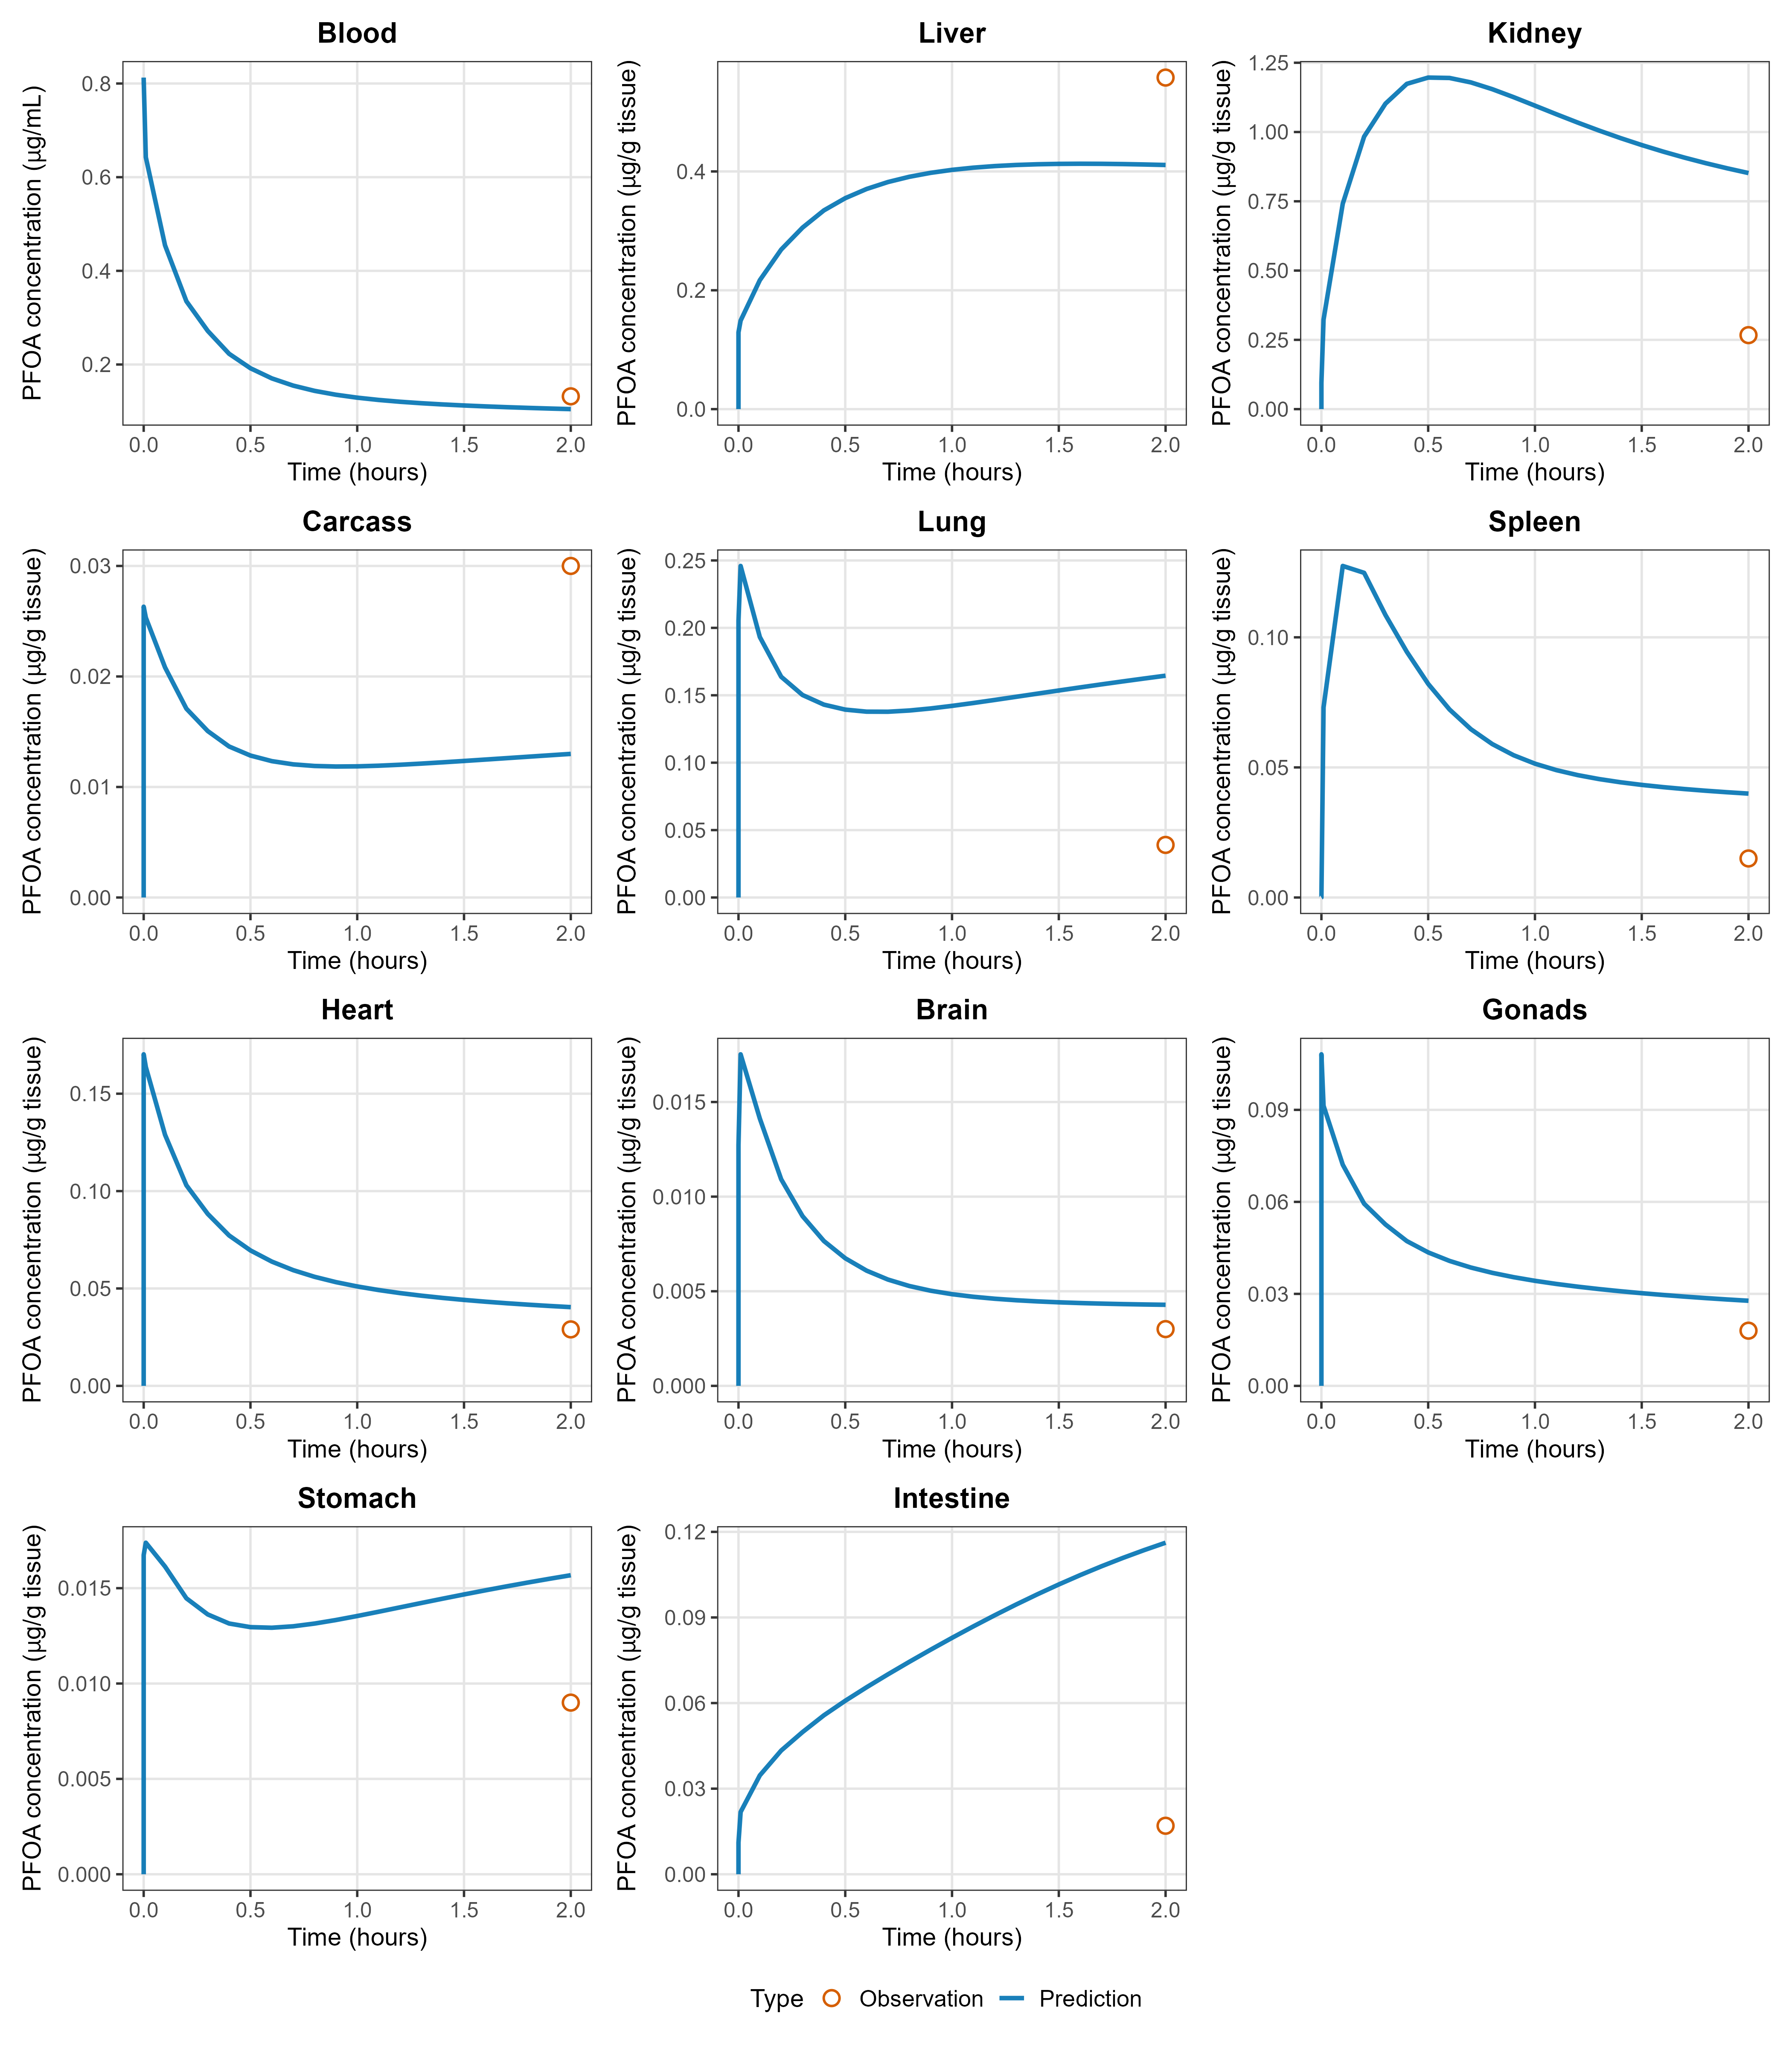
\includegraphics[width=1.0\textwidth]{sup_figures/experiment2.png}
    \caption{Model predictions versus observed tissue concentrations following intravenous injection in male rats. The applied dose was 0.04 $\text{mg}/\text{kg}$. Experimental data were obtained from \citet{kudo_2007}. The average prediction AAFE was 2.19.}
    \label{fig:experiment2}
\end{figure}


\begin{figure}[H]
    \centering
    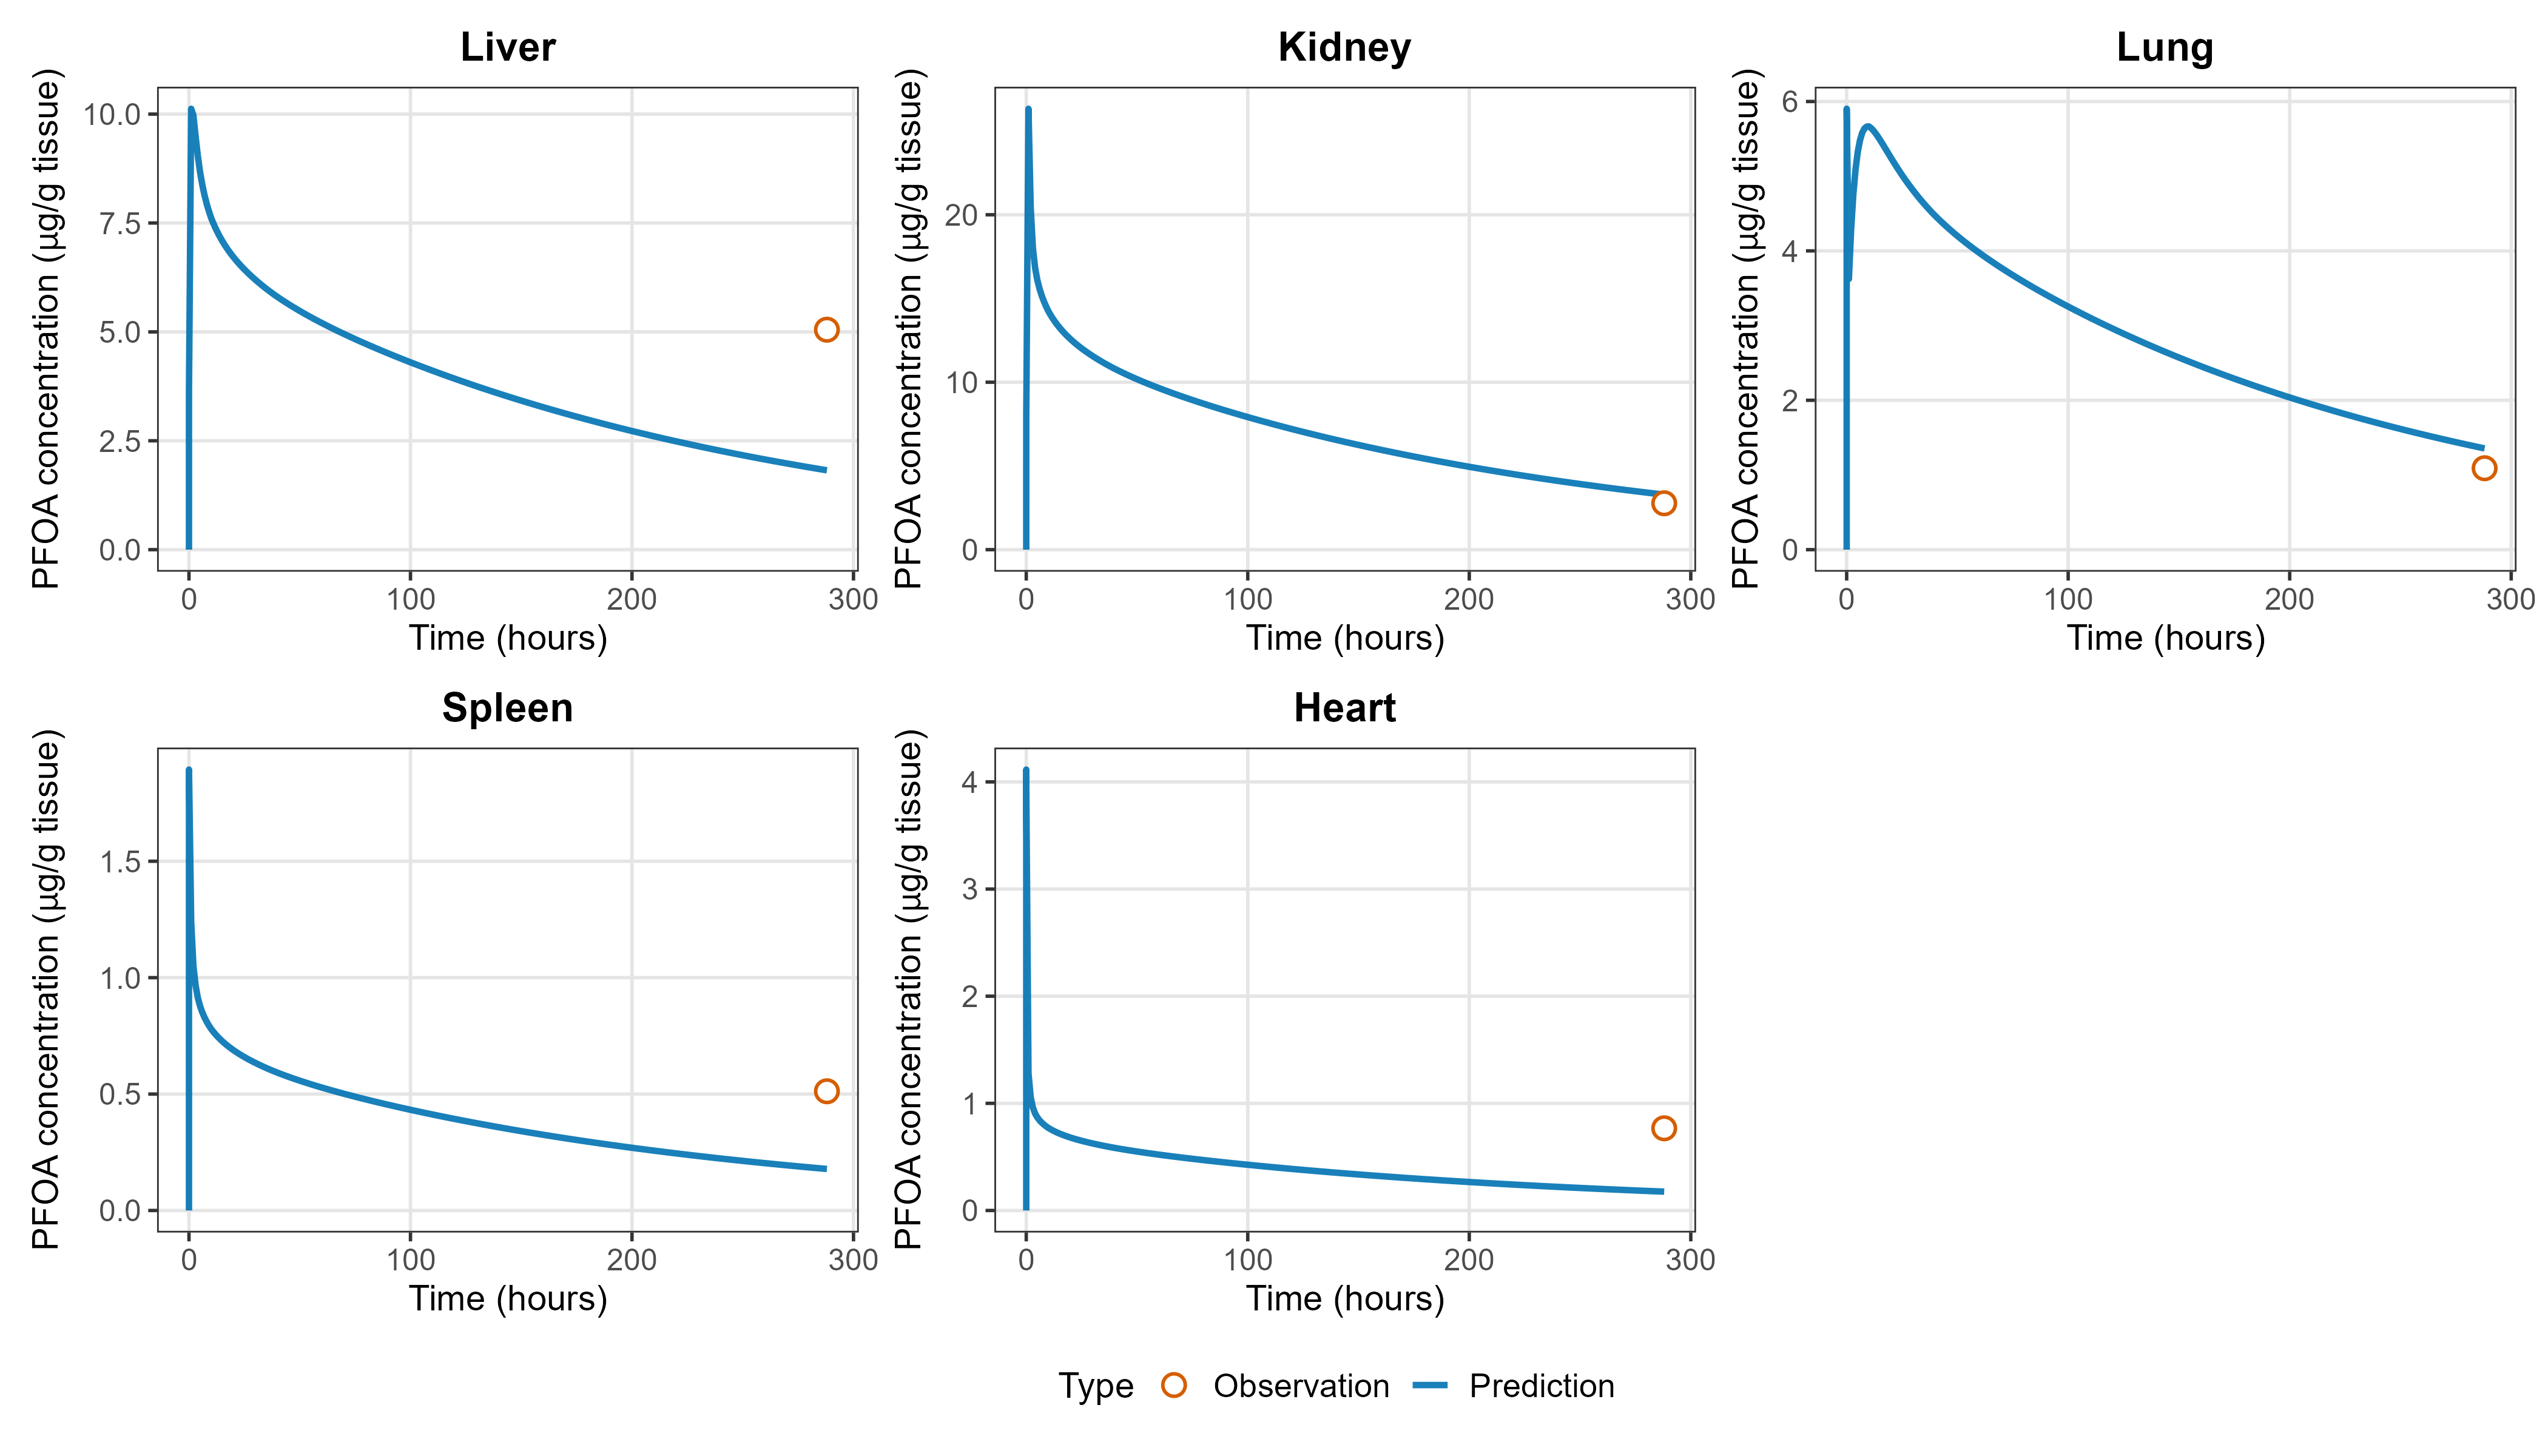
\includegraphics[width=1.0\textwidth]{sup_figures/experiment3.png}
    \caption{Model predictions versus observed tissue concentrations following IV injection in male rats. The applied dose was 1 $\text{mg}/\text{kg}$. Experimental data were obtained from \citet{kim_2016}. The average prediction AAFE was 2.19.}
    \label{fig:experiment3}
\end{figure}


\begin{figure}[H]
    \centering
    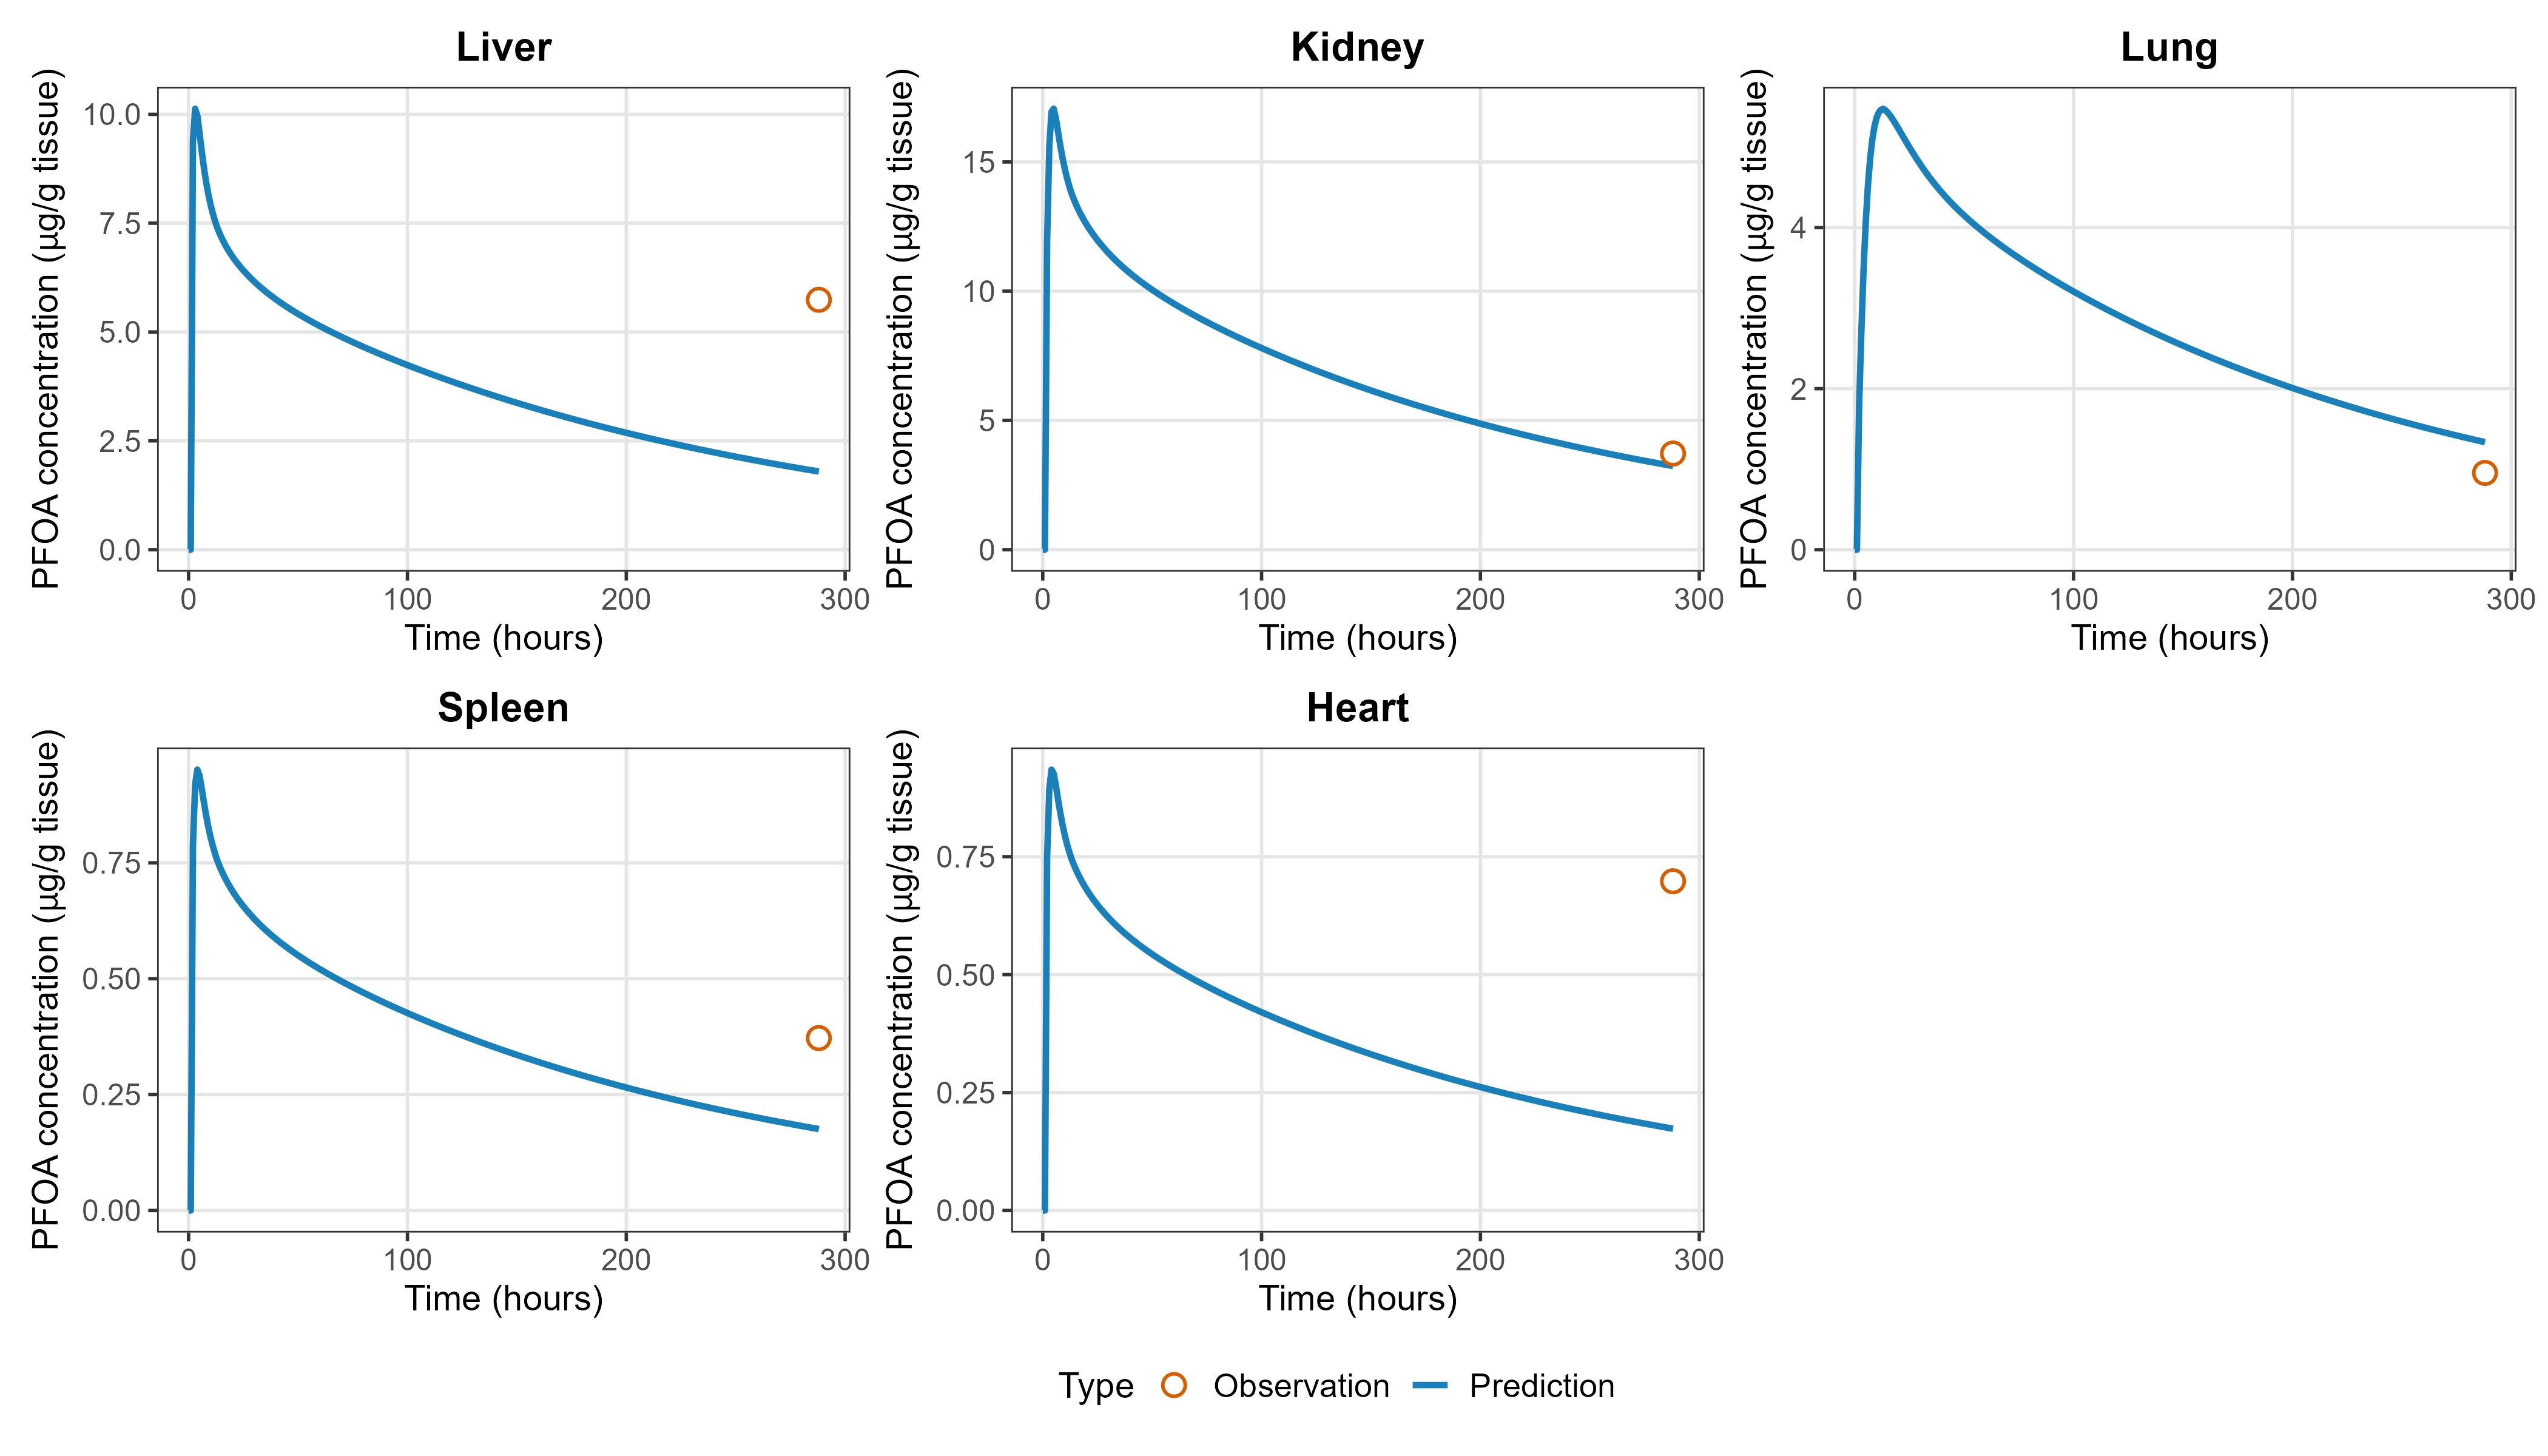
\includegraphics[width=1.0\textwidth]{sup_figures/experiment4.png}
    \caption{Model predictions versus observed tissue concentrations following oral ingestion in male rats. The applied dose was 1 $\text{mg}/\text{kg}$. Experimental data were obtained from \citet{kim_2016}. The average prediction AAFE was 2.13.}
    \label{fig:experiment4}
\end{figure}


\begin{figure}[H]
    \centering
    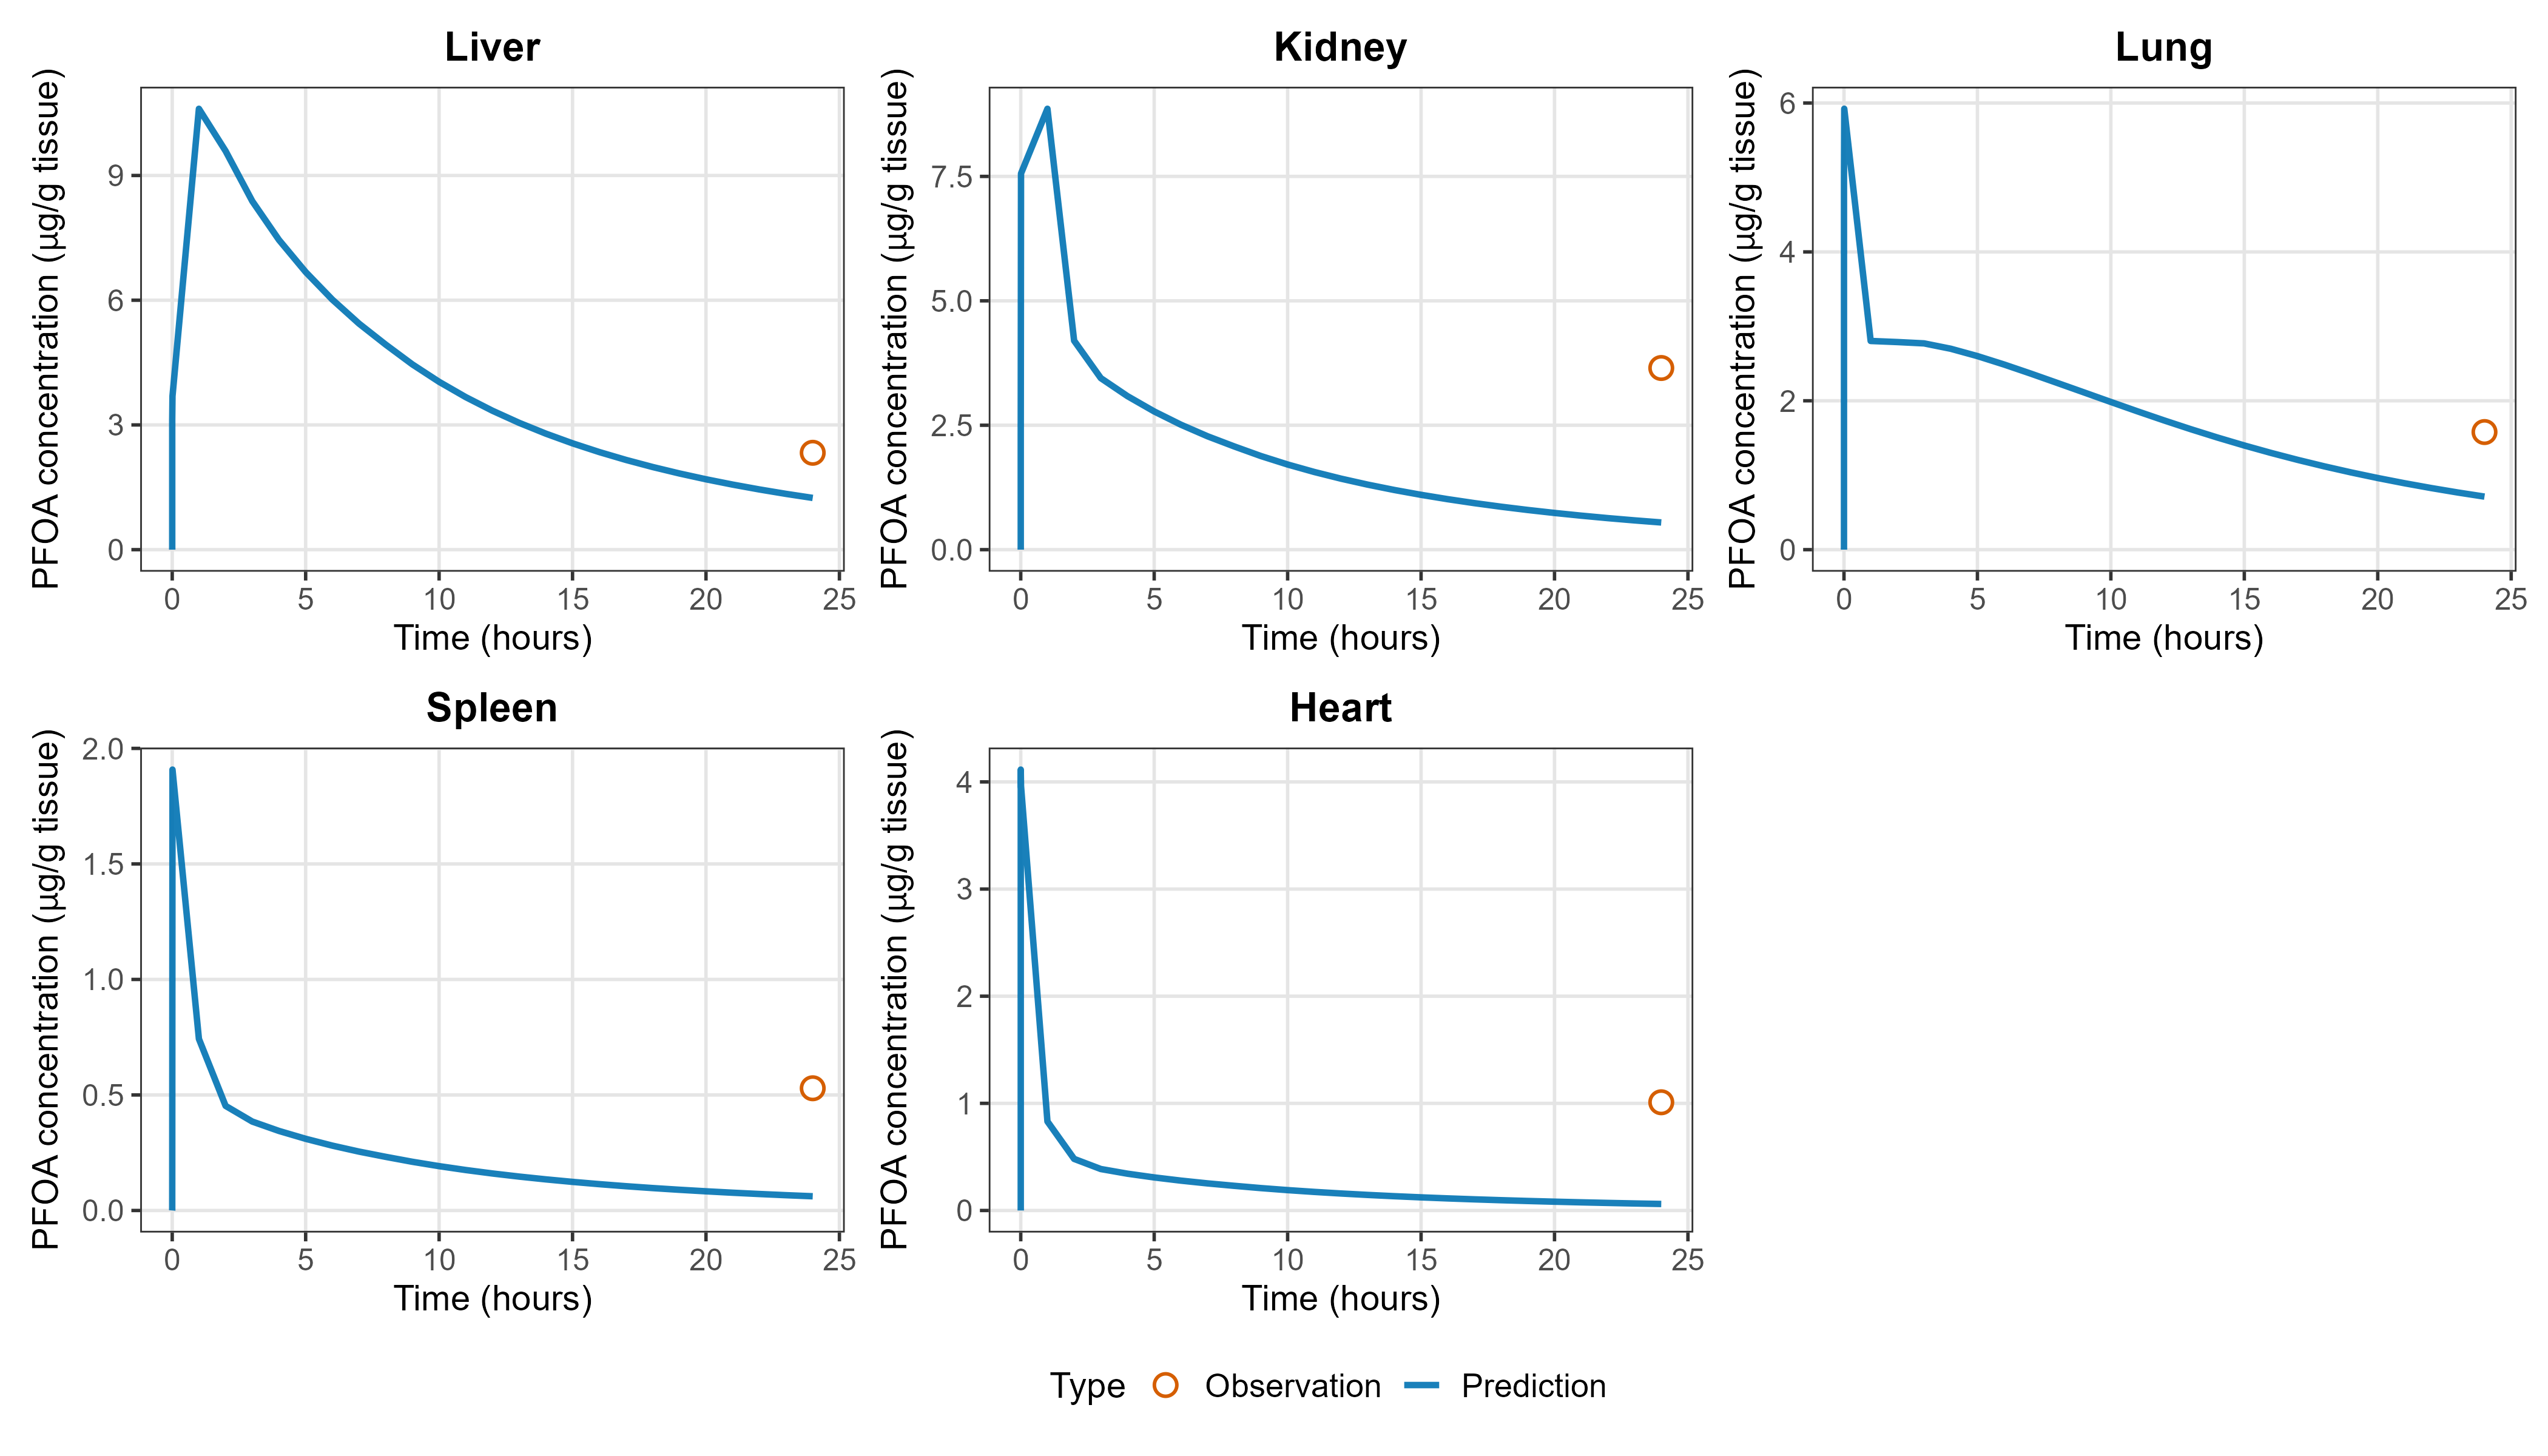
\includegraphics[width=1.0\textwidth]{sup_figures/experiment5.png}
    \caption{Model predictions versus observed tissue concentrations following IV injection in female rats. The applied dose was 1 $\text{mg}/\text{kg}$. Experimental data were obtained from \citet{kim_2016}. The average prediction AAFE was 5.29.}
    \label{fig:experiment5}
\end{figure}


\begin{figure}[H]
    \centering
    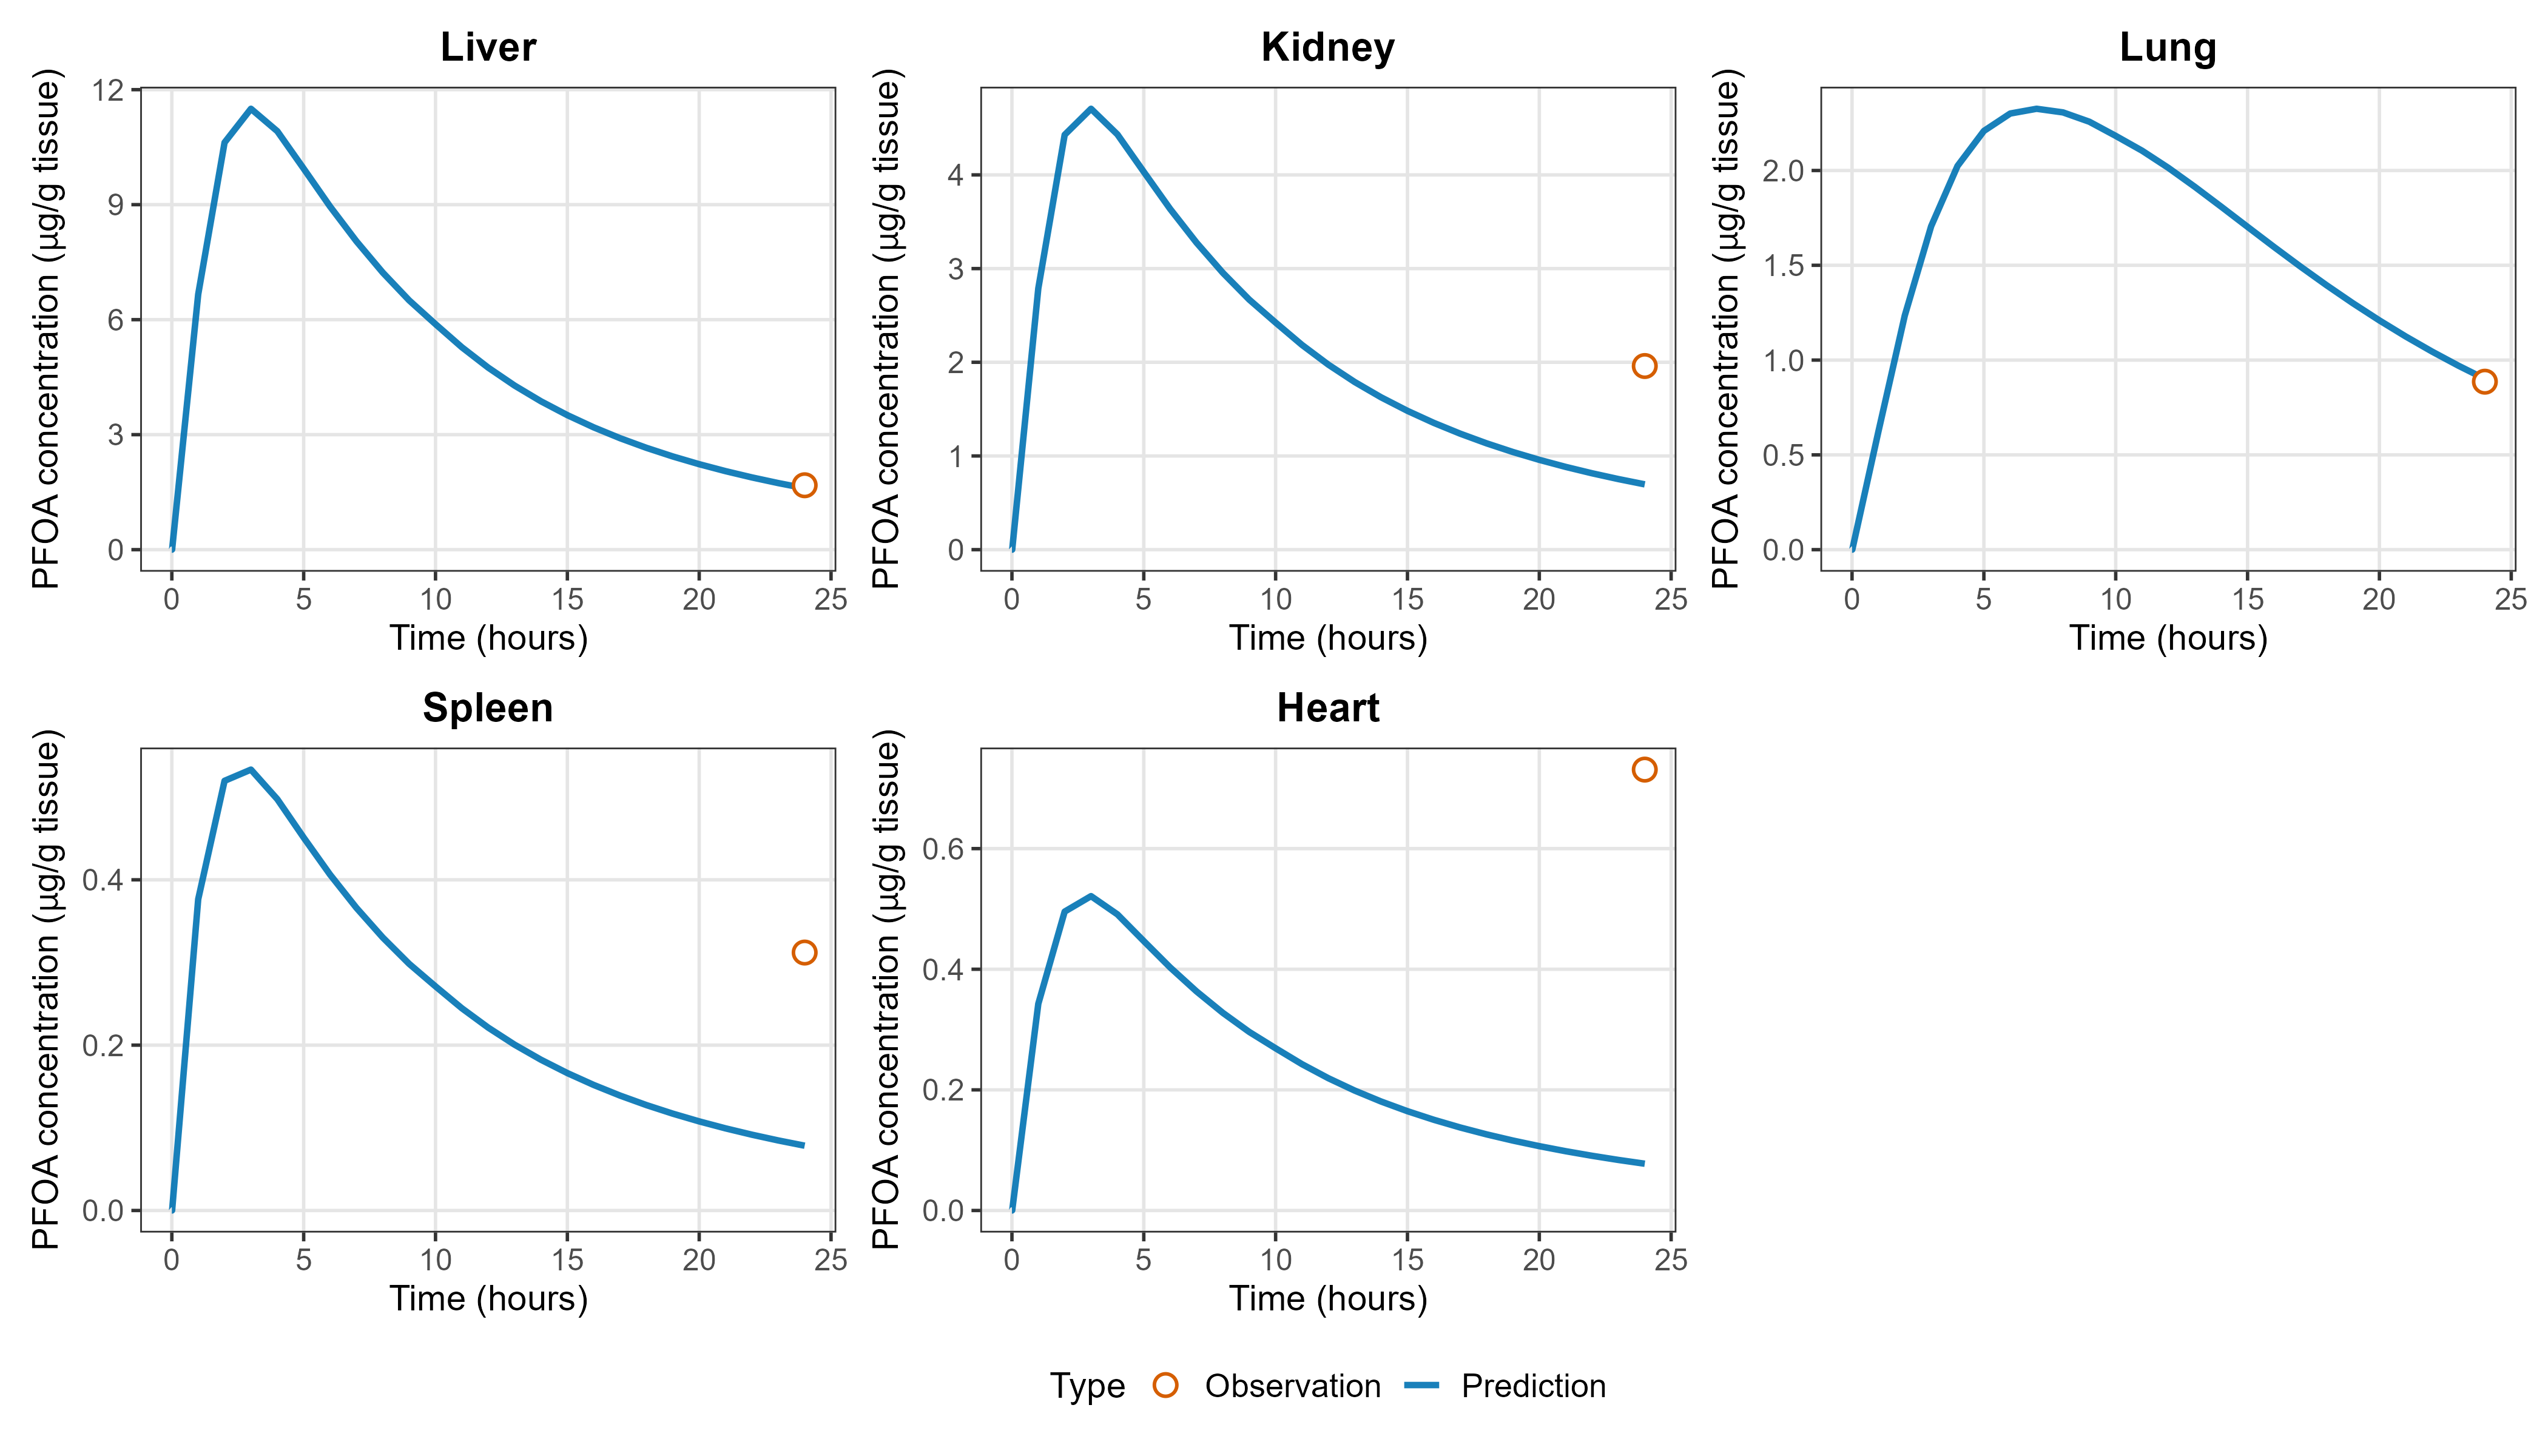
\includegraphics[width=1.0\textwidth]{sup_figures/experiment6.png}
    \caption{Model predictions versus observed tissue concentrations following oral ingestion in female rats. The applied dose was 1 $\text{mg}/\text{kg}$. Experimental data were obtained from \citet{kim_2016}. The average prediction AAFE was 2.59.}
    \label{fig:experiment6}
\end{figure}



\begin{figure}[H]
    \centering
    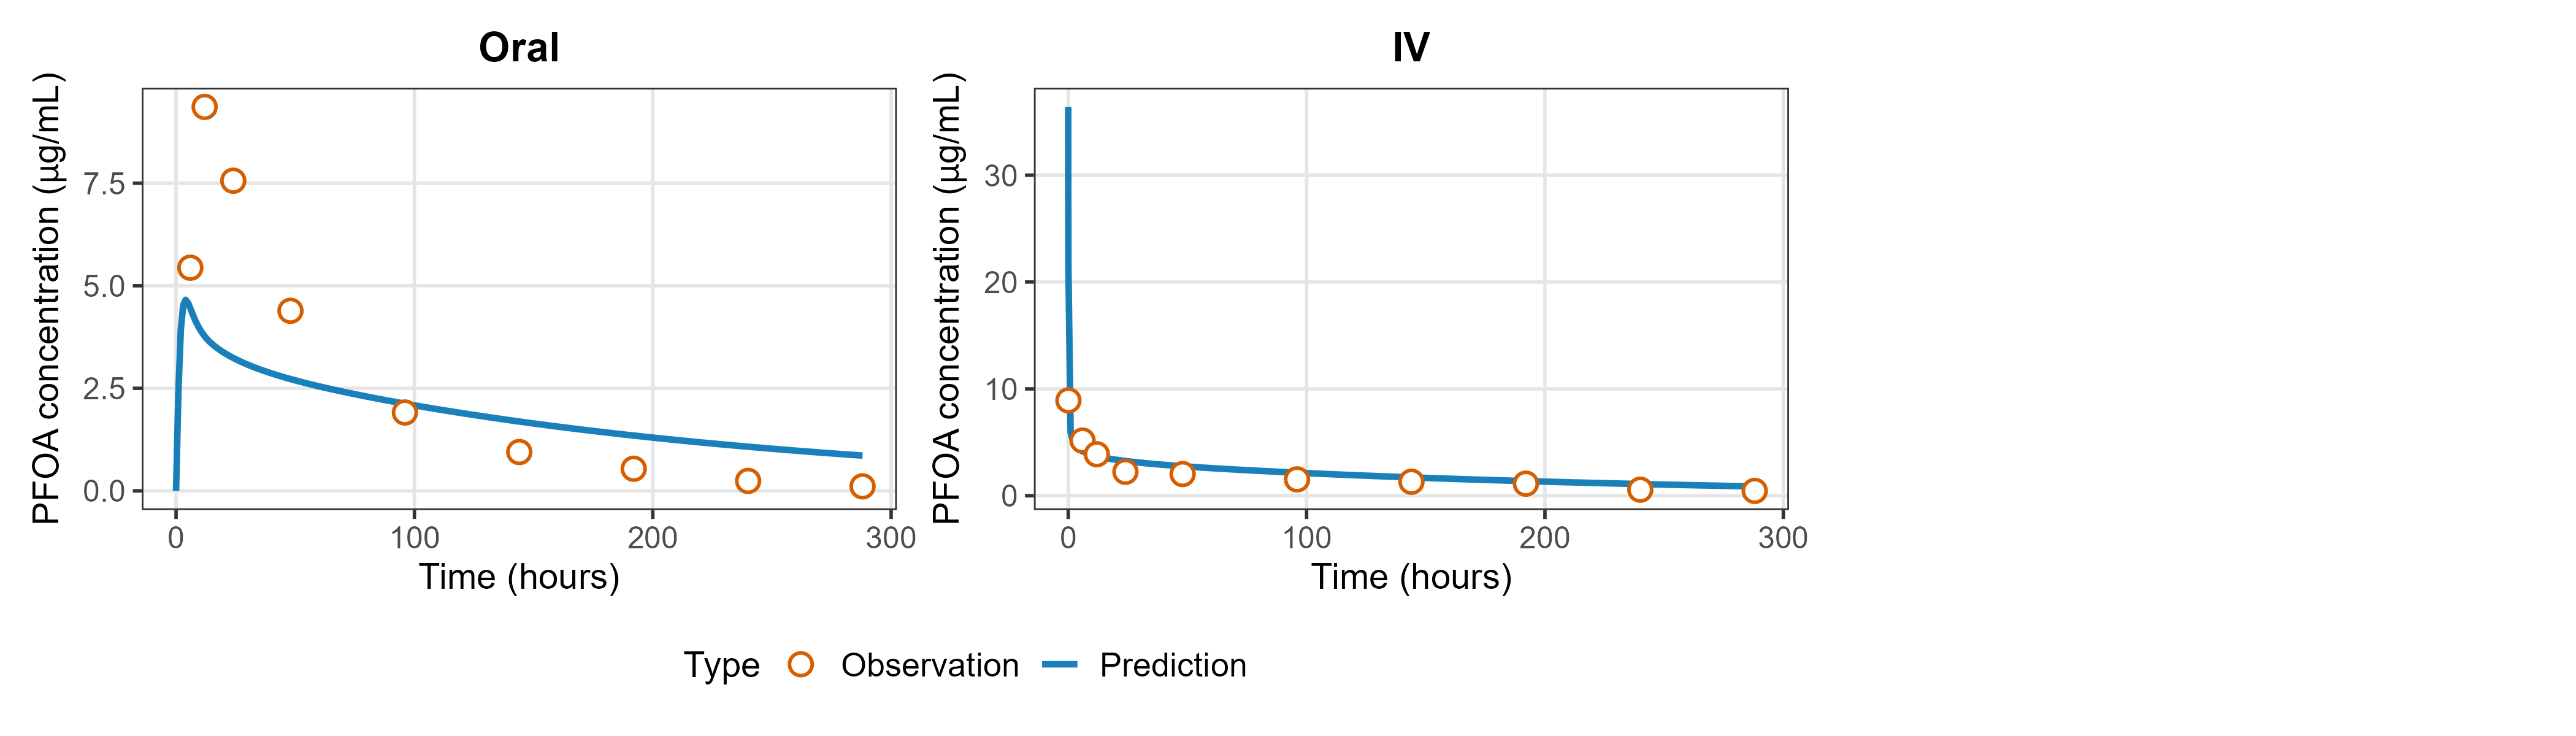
\includegraphics[width=1.0\textwidth]{sup_figures/experiment9.png}
    \caption{Model predictions versus observed plasma concentrations following oral ingestion (left) and IV injection (right) in male rats. The applied dose was 1 $\text{mg}/\text{kg}$. Experimental data were obtained from \citet{kim_2016}. The average prediction AAFE was 1.88.}
    \label{fig:experiment9}
\end{figure}


\begin{figure}[H]
    \centering
    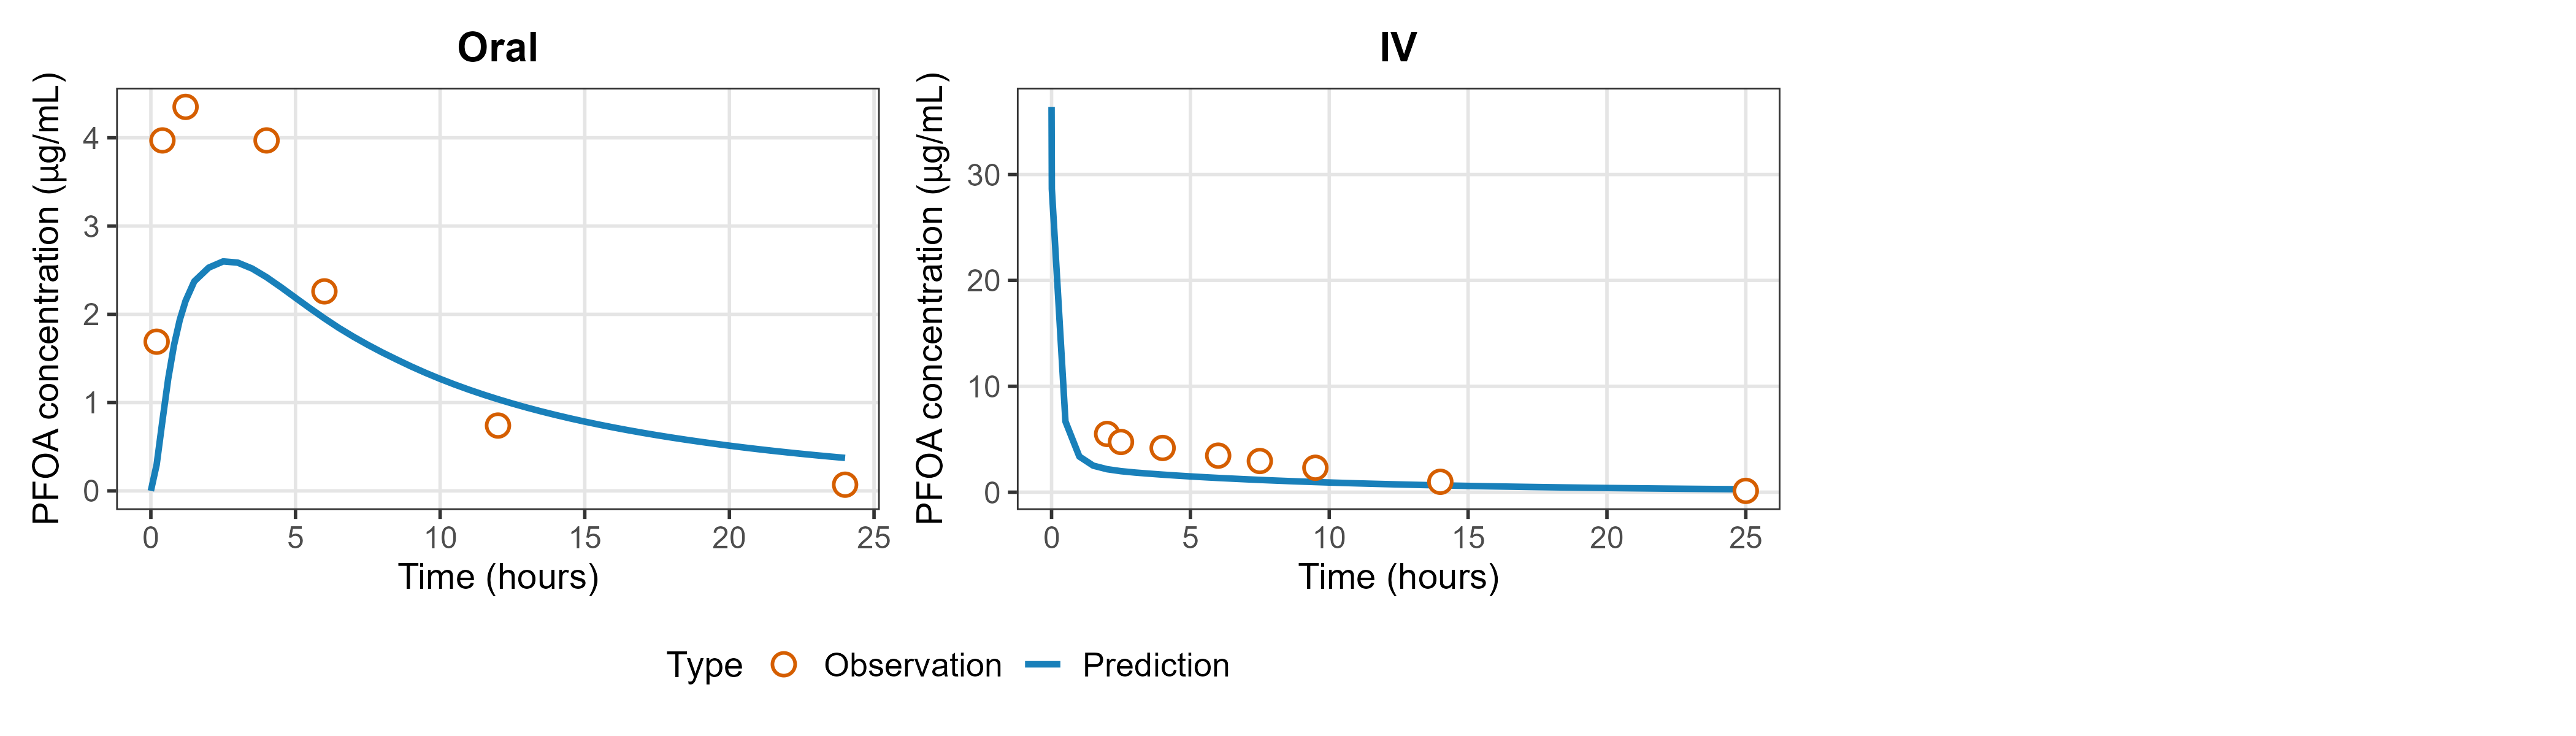
\includegraphics[width=1.0\textwidth]{sup_figures/experiment12.png}
    \caption{Model predictions versus observed plasma concentrations following oral ingestion (left) and IV injection (right) in female rats. The applied dose was 1 $\text{mg}/\text{kg}$. Experimental data were obtained from \citet{kim_2016}. The average prediction AAFE was 2.45.}
    \label{fig:experiment12}
\end{figure}


\begin{figure}[H]
    \centering
    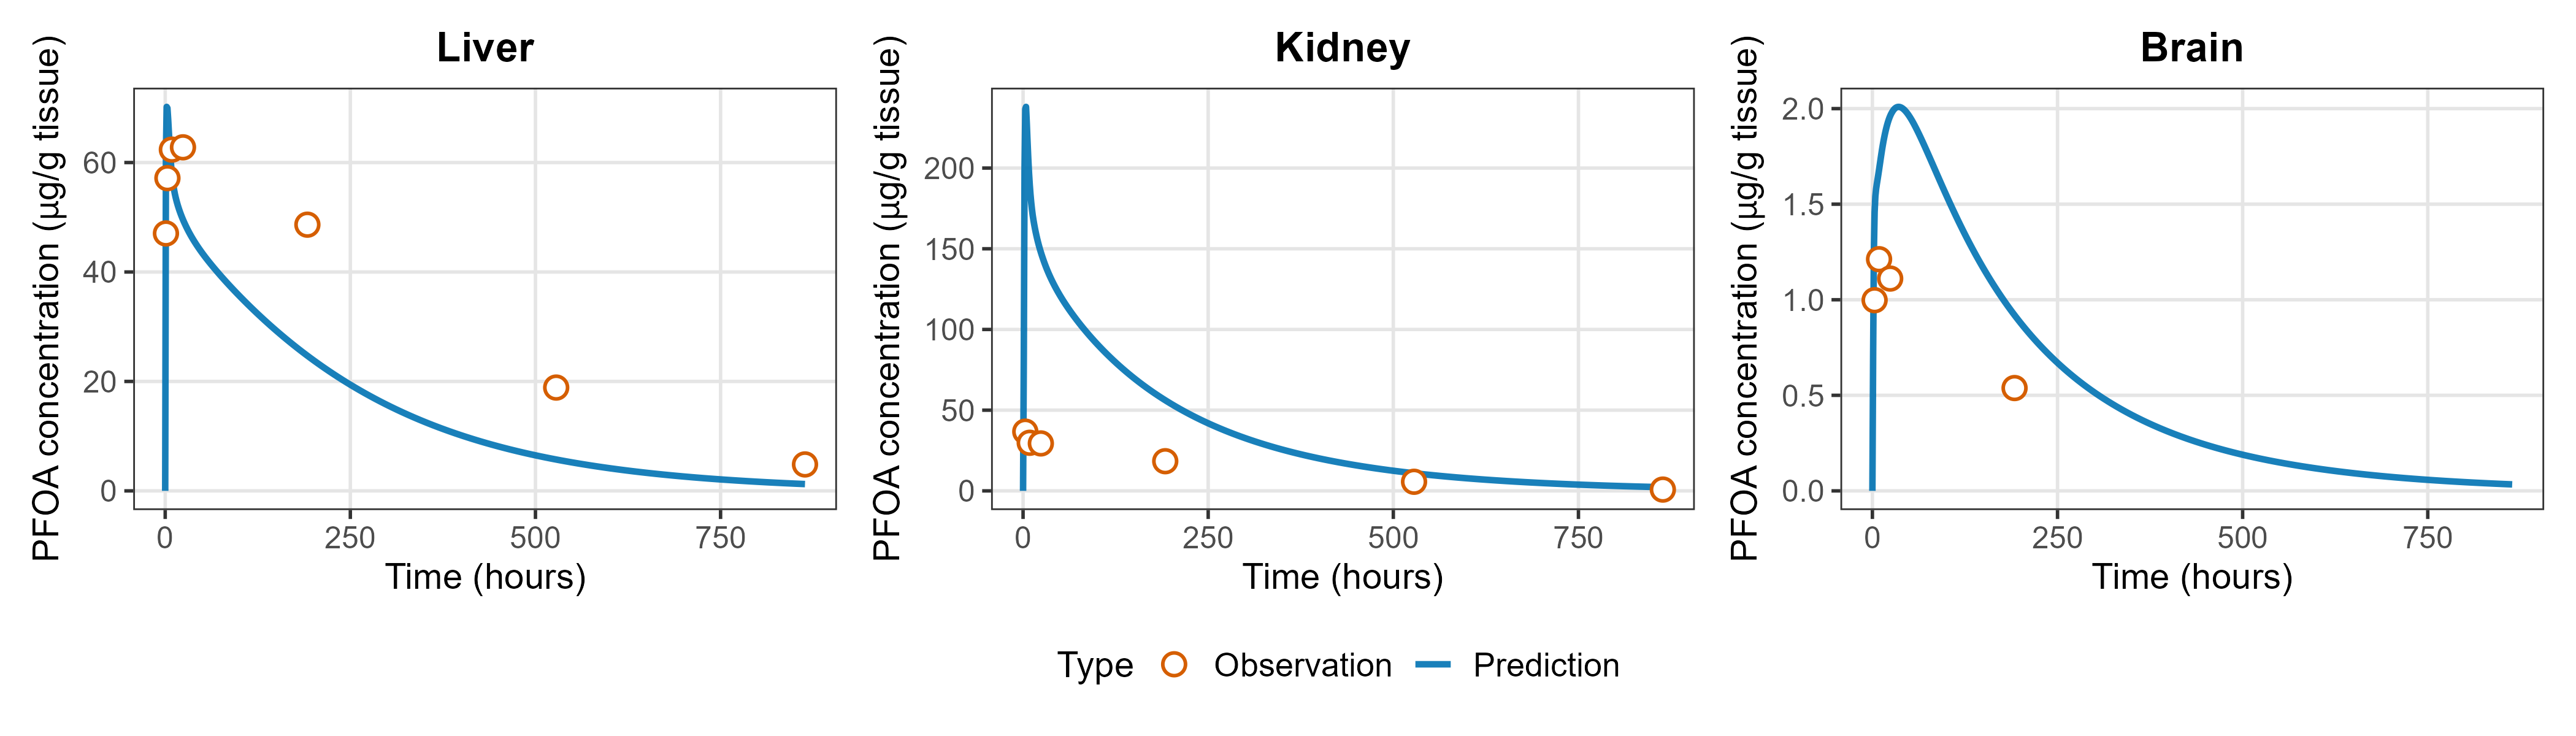
\includegraphics[width=1.0\textwidth]{sup_figures/experiment7.png}
    \caption{Model predictions versus observed tissue concentrations following oral ingestion in male rats. The applied dose was 12 $\text{mg}/\text{kg}$. Experimental data were obtained from \citet{dzierlenga_2020}. The average prediction AAFE was 2.27.}
    \label{fig:experiment7}
\end{figure}


\begin{figure}[H]
    \centering
    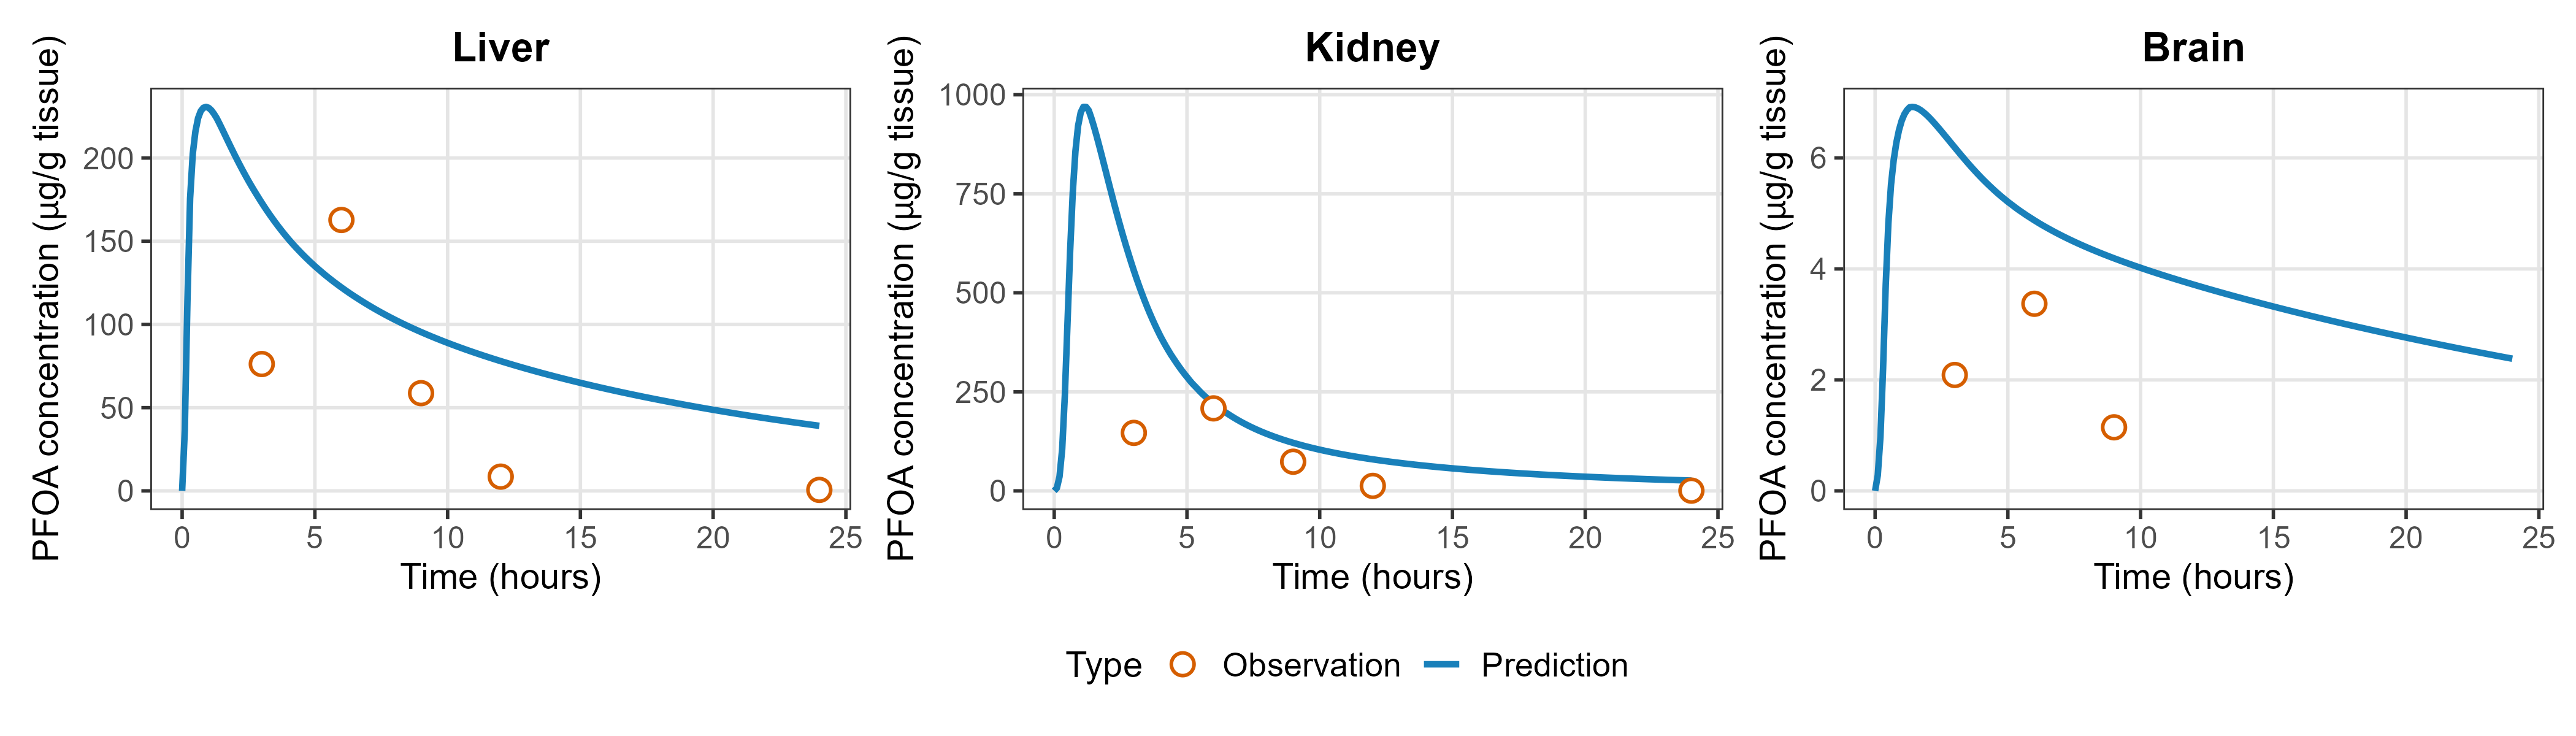
\includegraphics[width=1.0\textwidth]{sup_figures/experiment8.png}
    \caption{Model predictions versus observed tissue concentrations following oral ingestion in female rats. The applied dose was 80 $\text{mg}/\text{kg}$. Experimental data were obtained from \citet{dzierlenga_2020}. The average prediction AAFE was 4.07.}
    \label{fig:experiment8}
\end{figure}





\begin{figure}[H]
    \centering
    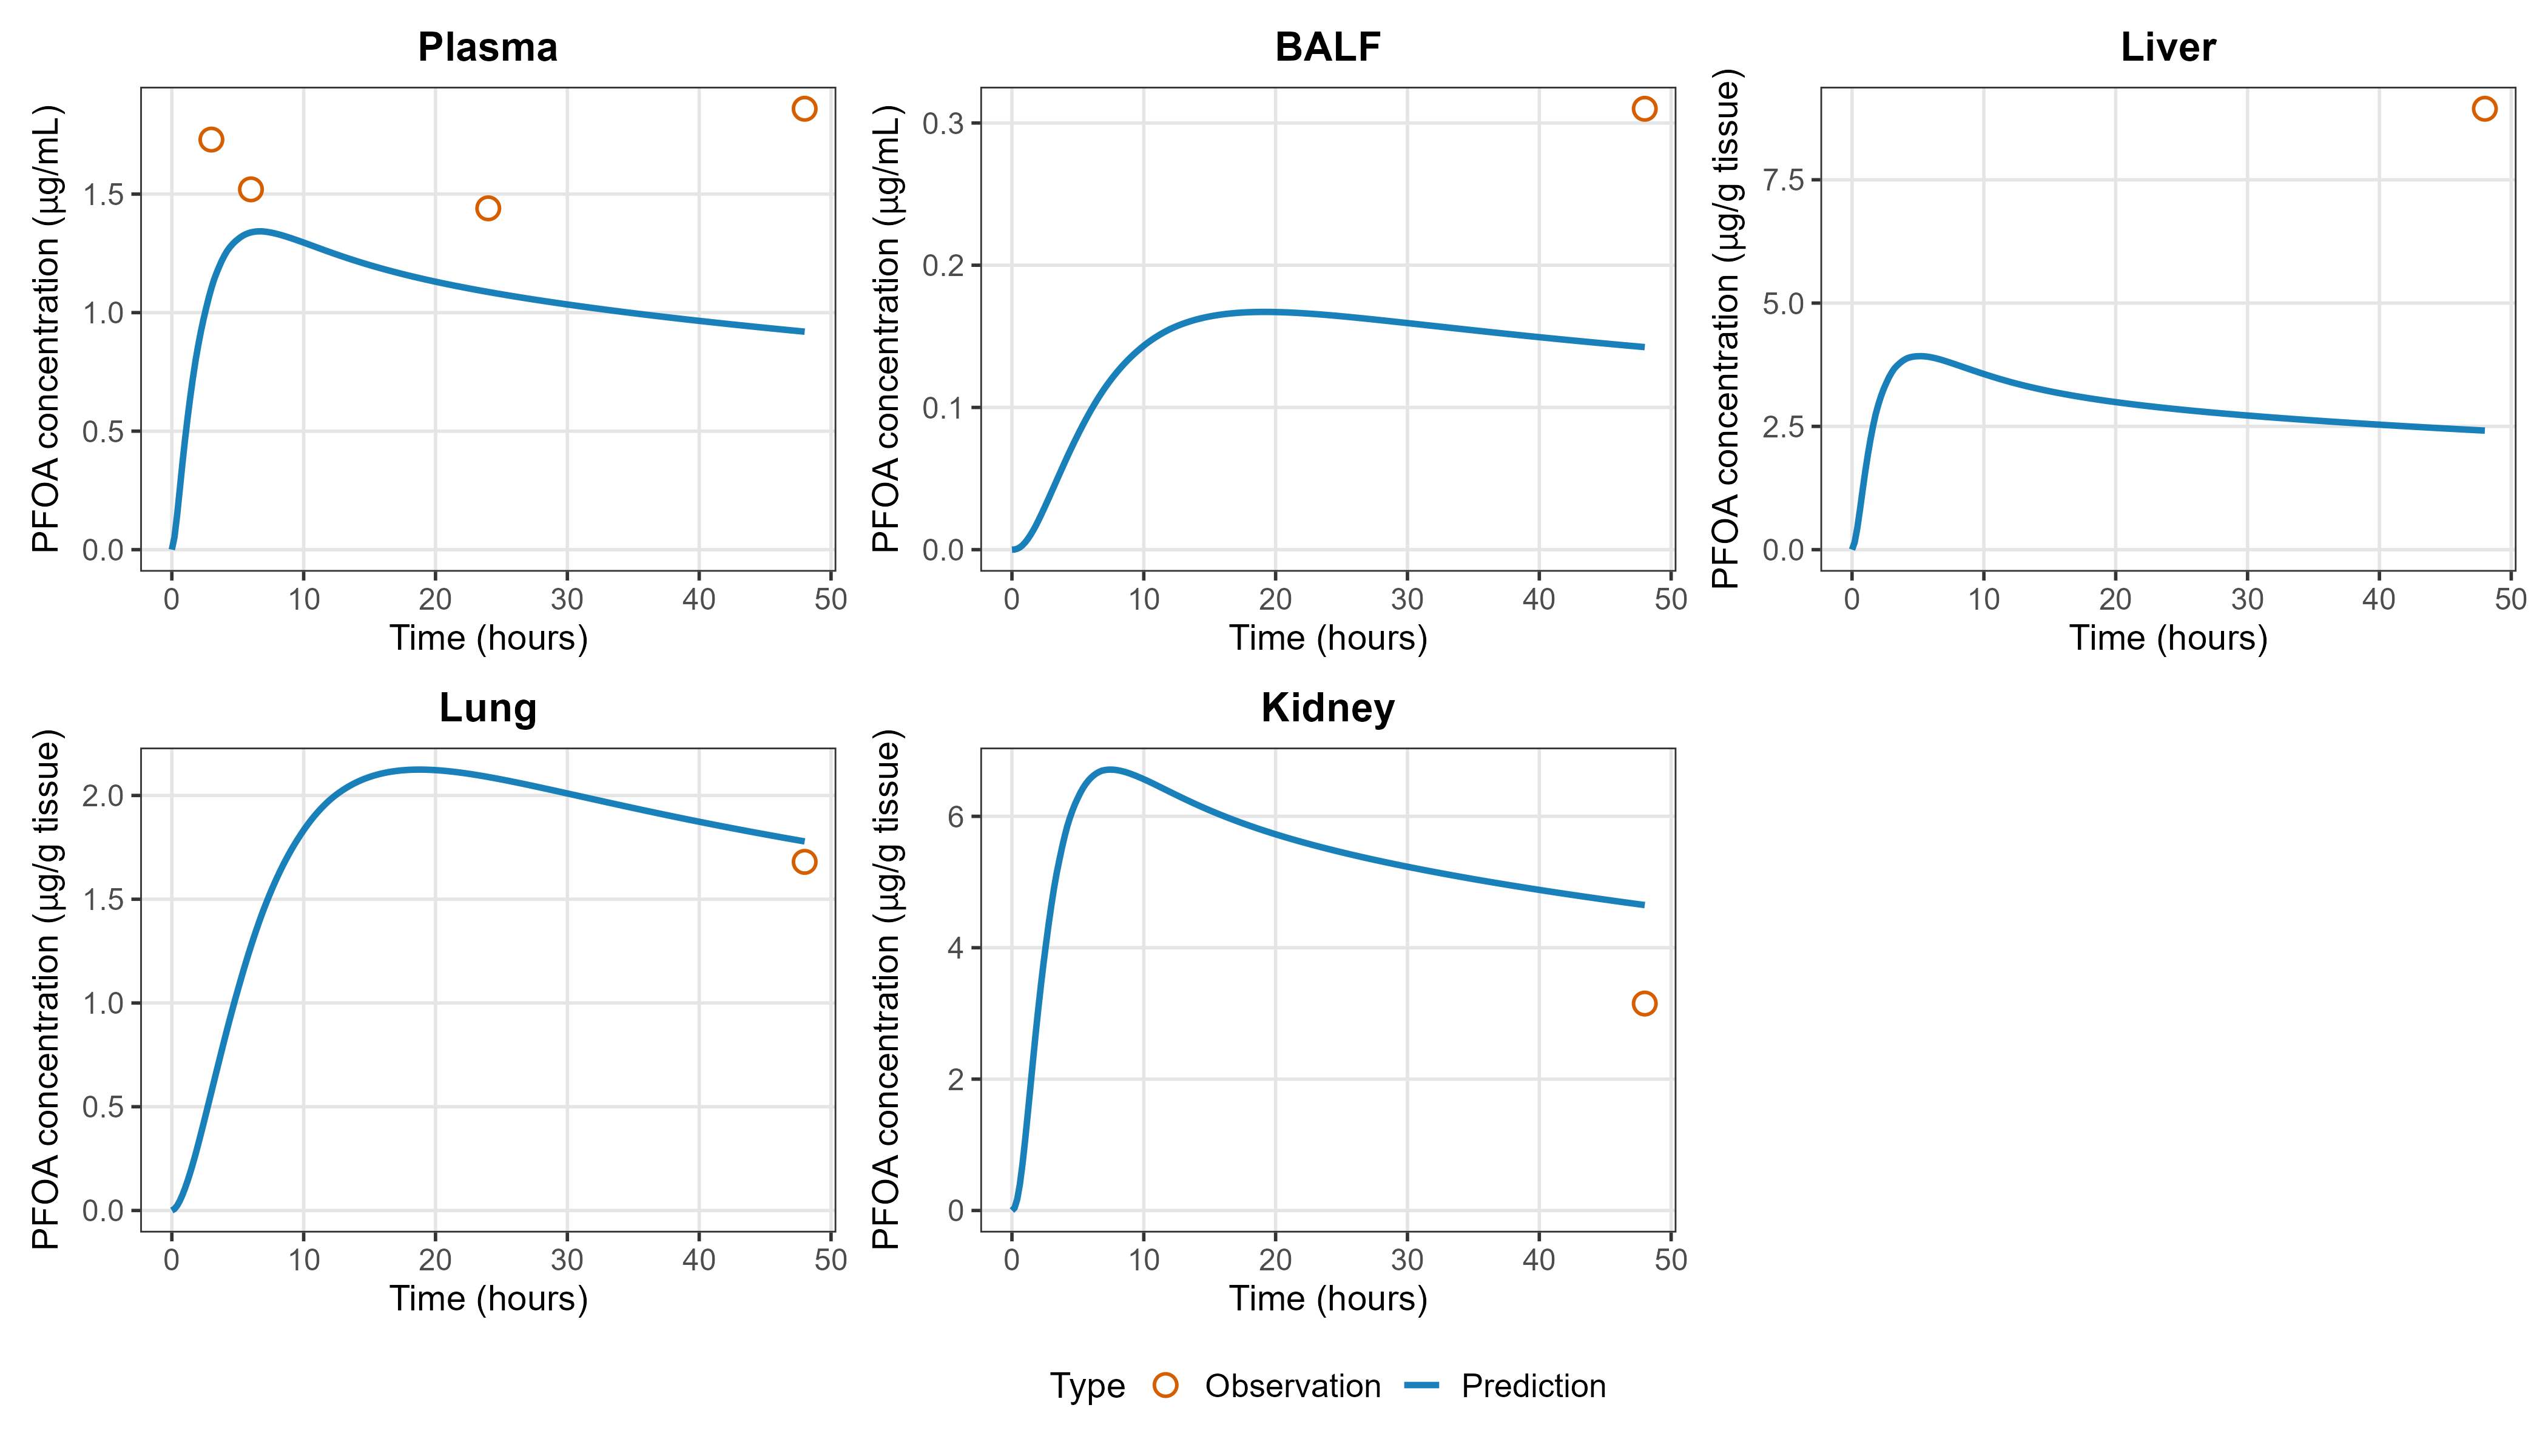
\includegraphics[width=1.0\textwidth]{sup_figures/experiment13.png}
    \caption{Model predictions versus observed plasma and tissue concentrations following oral ingestion in male rats. The applied dose was 0.364 $\text{mg}/\text{kg}$. Experimental data were obtained from \citet{gustafsson_2022}. The average prediction AAFE was 3.16.}
    \label{fig:experiment13}
\end{figure}


\begin{figure}[H]
    \centering
    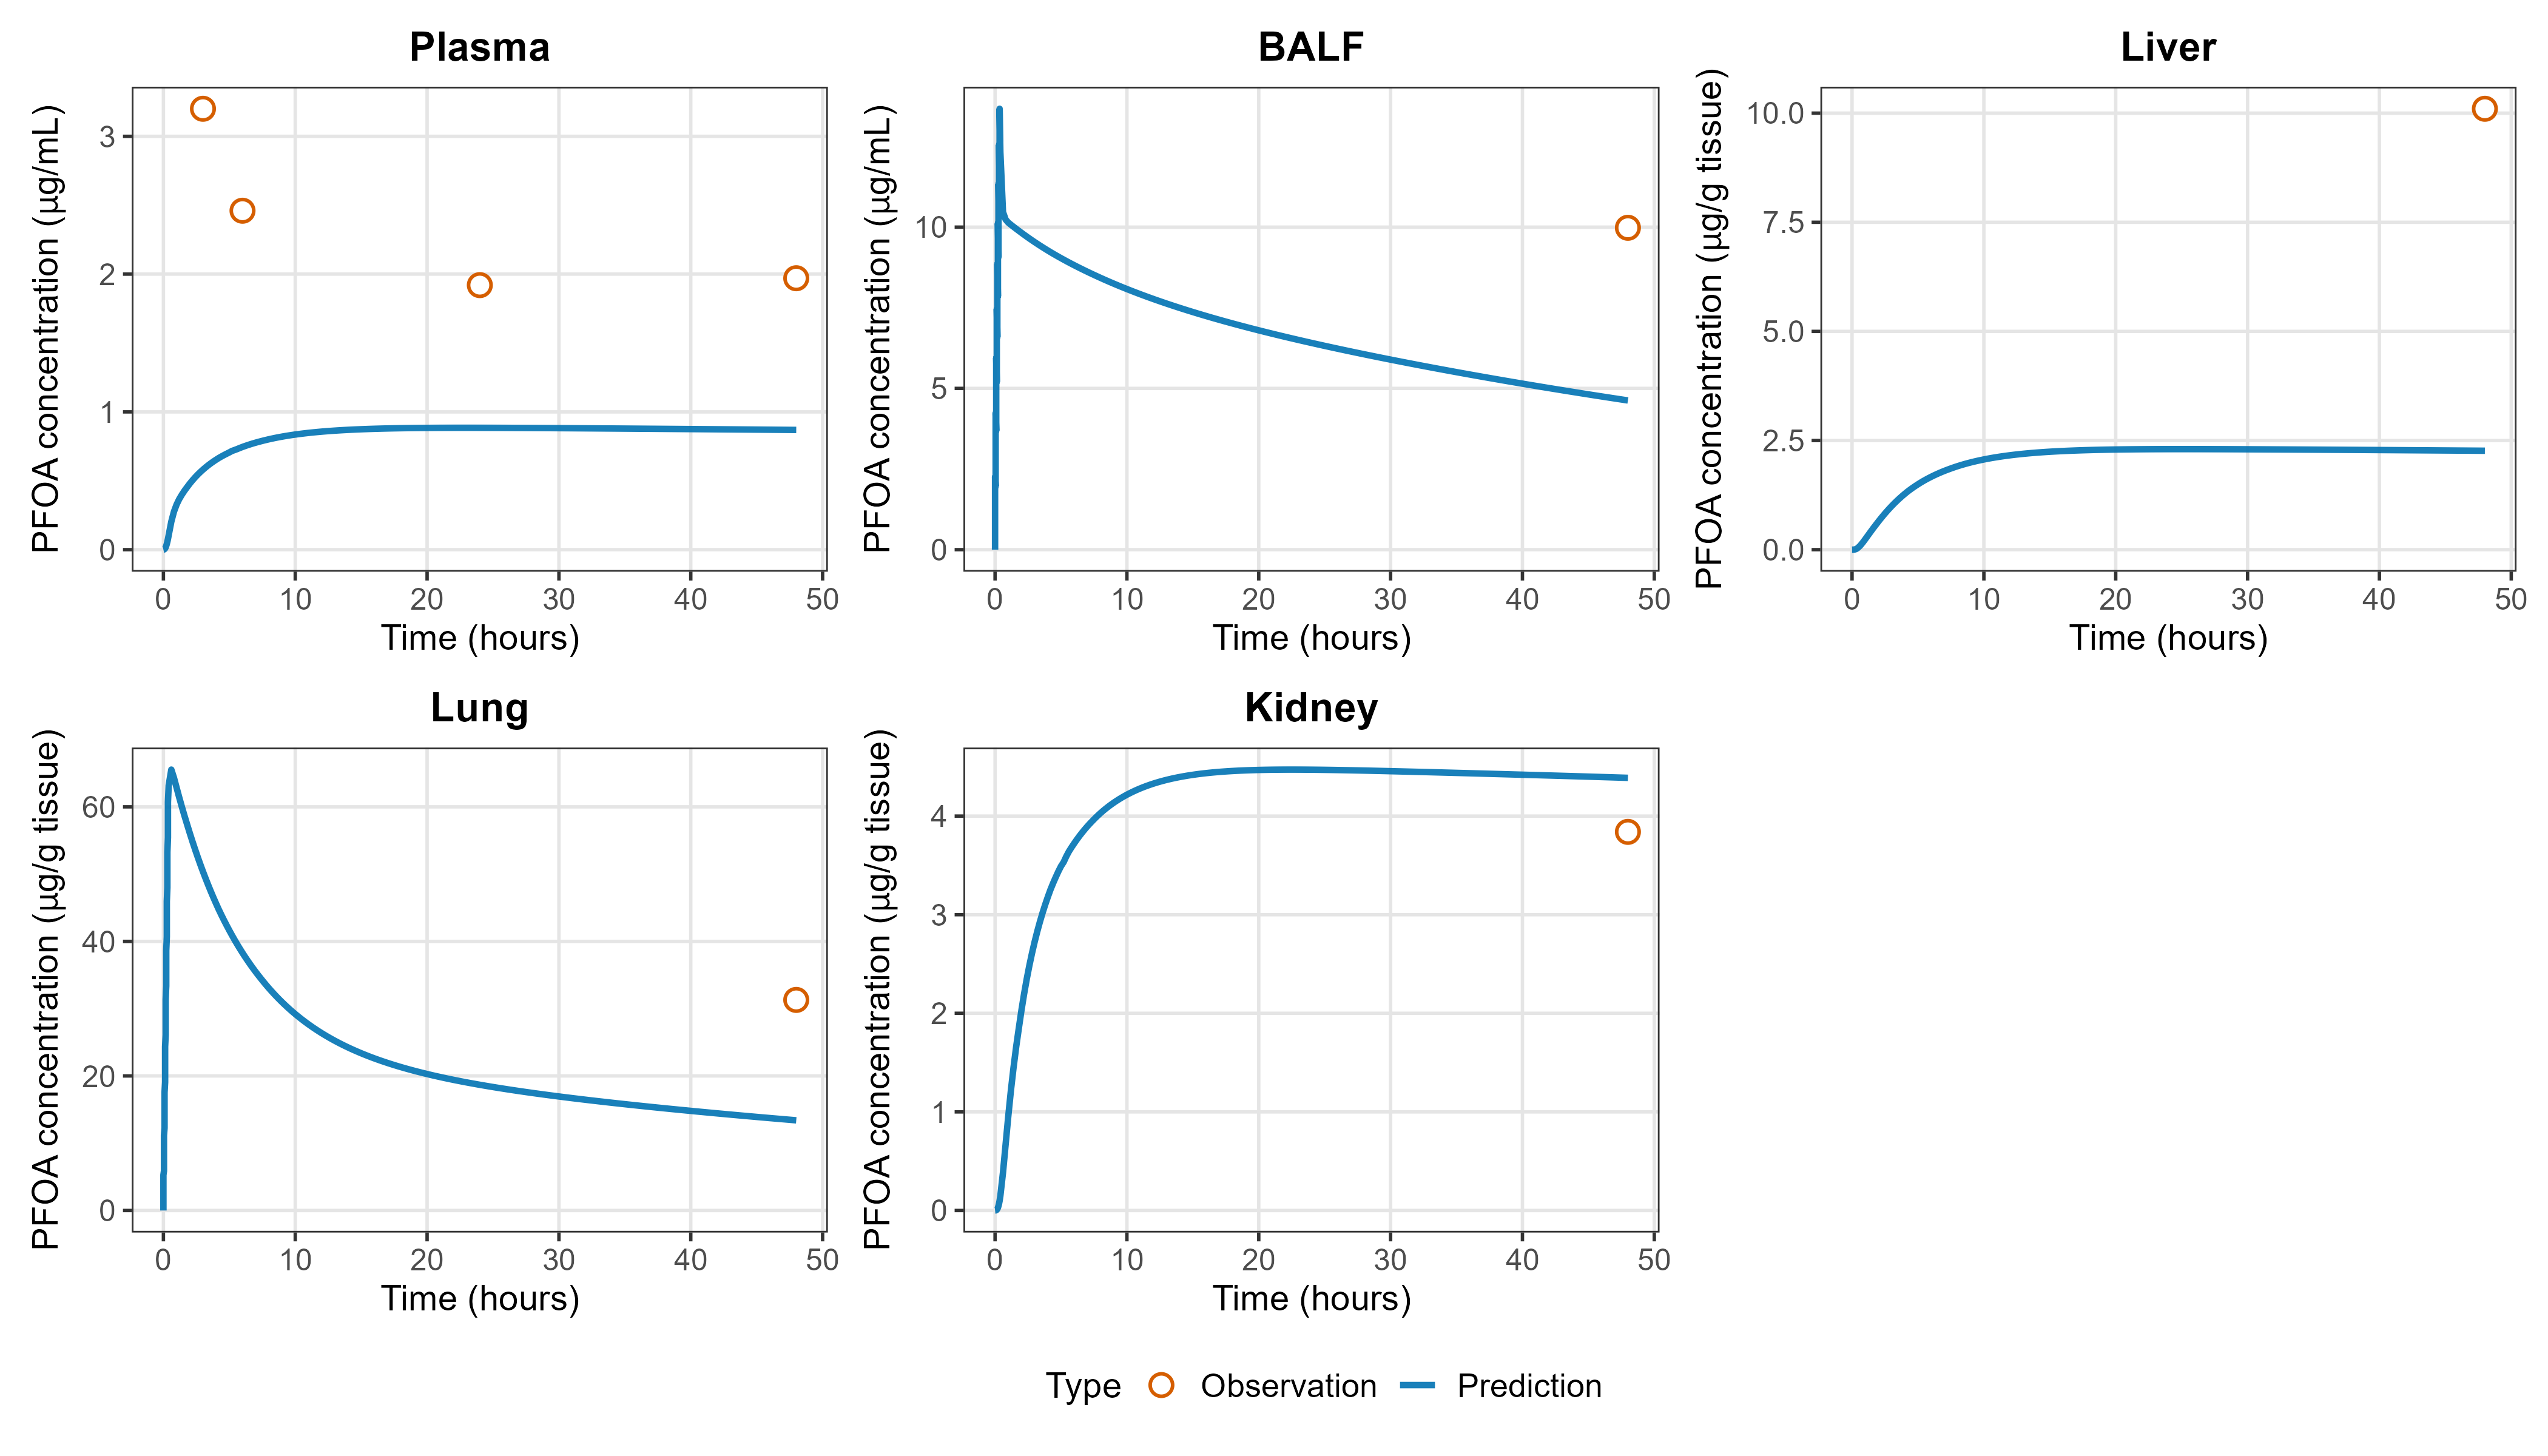
\includegraphics[width=1.0\textwidth]{sup_figures/experiment14.png}
    \caption{Model predictions versus observed tissue concentrations following inhalation in male rats. The deposited dose was 0.207 $\text{mg}/\text{kg}$. Experimental data were obtained from \citet{gustafsson_2022}. The average prediction AAFE was 2.65.}
    \label{fig:experiment14}
\end{figure}



\begin{figure}[H]
    \centering
    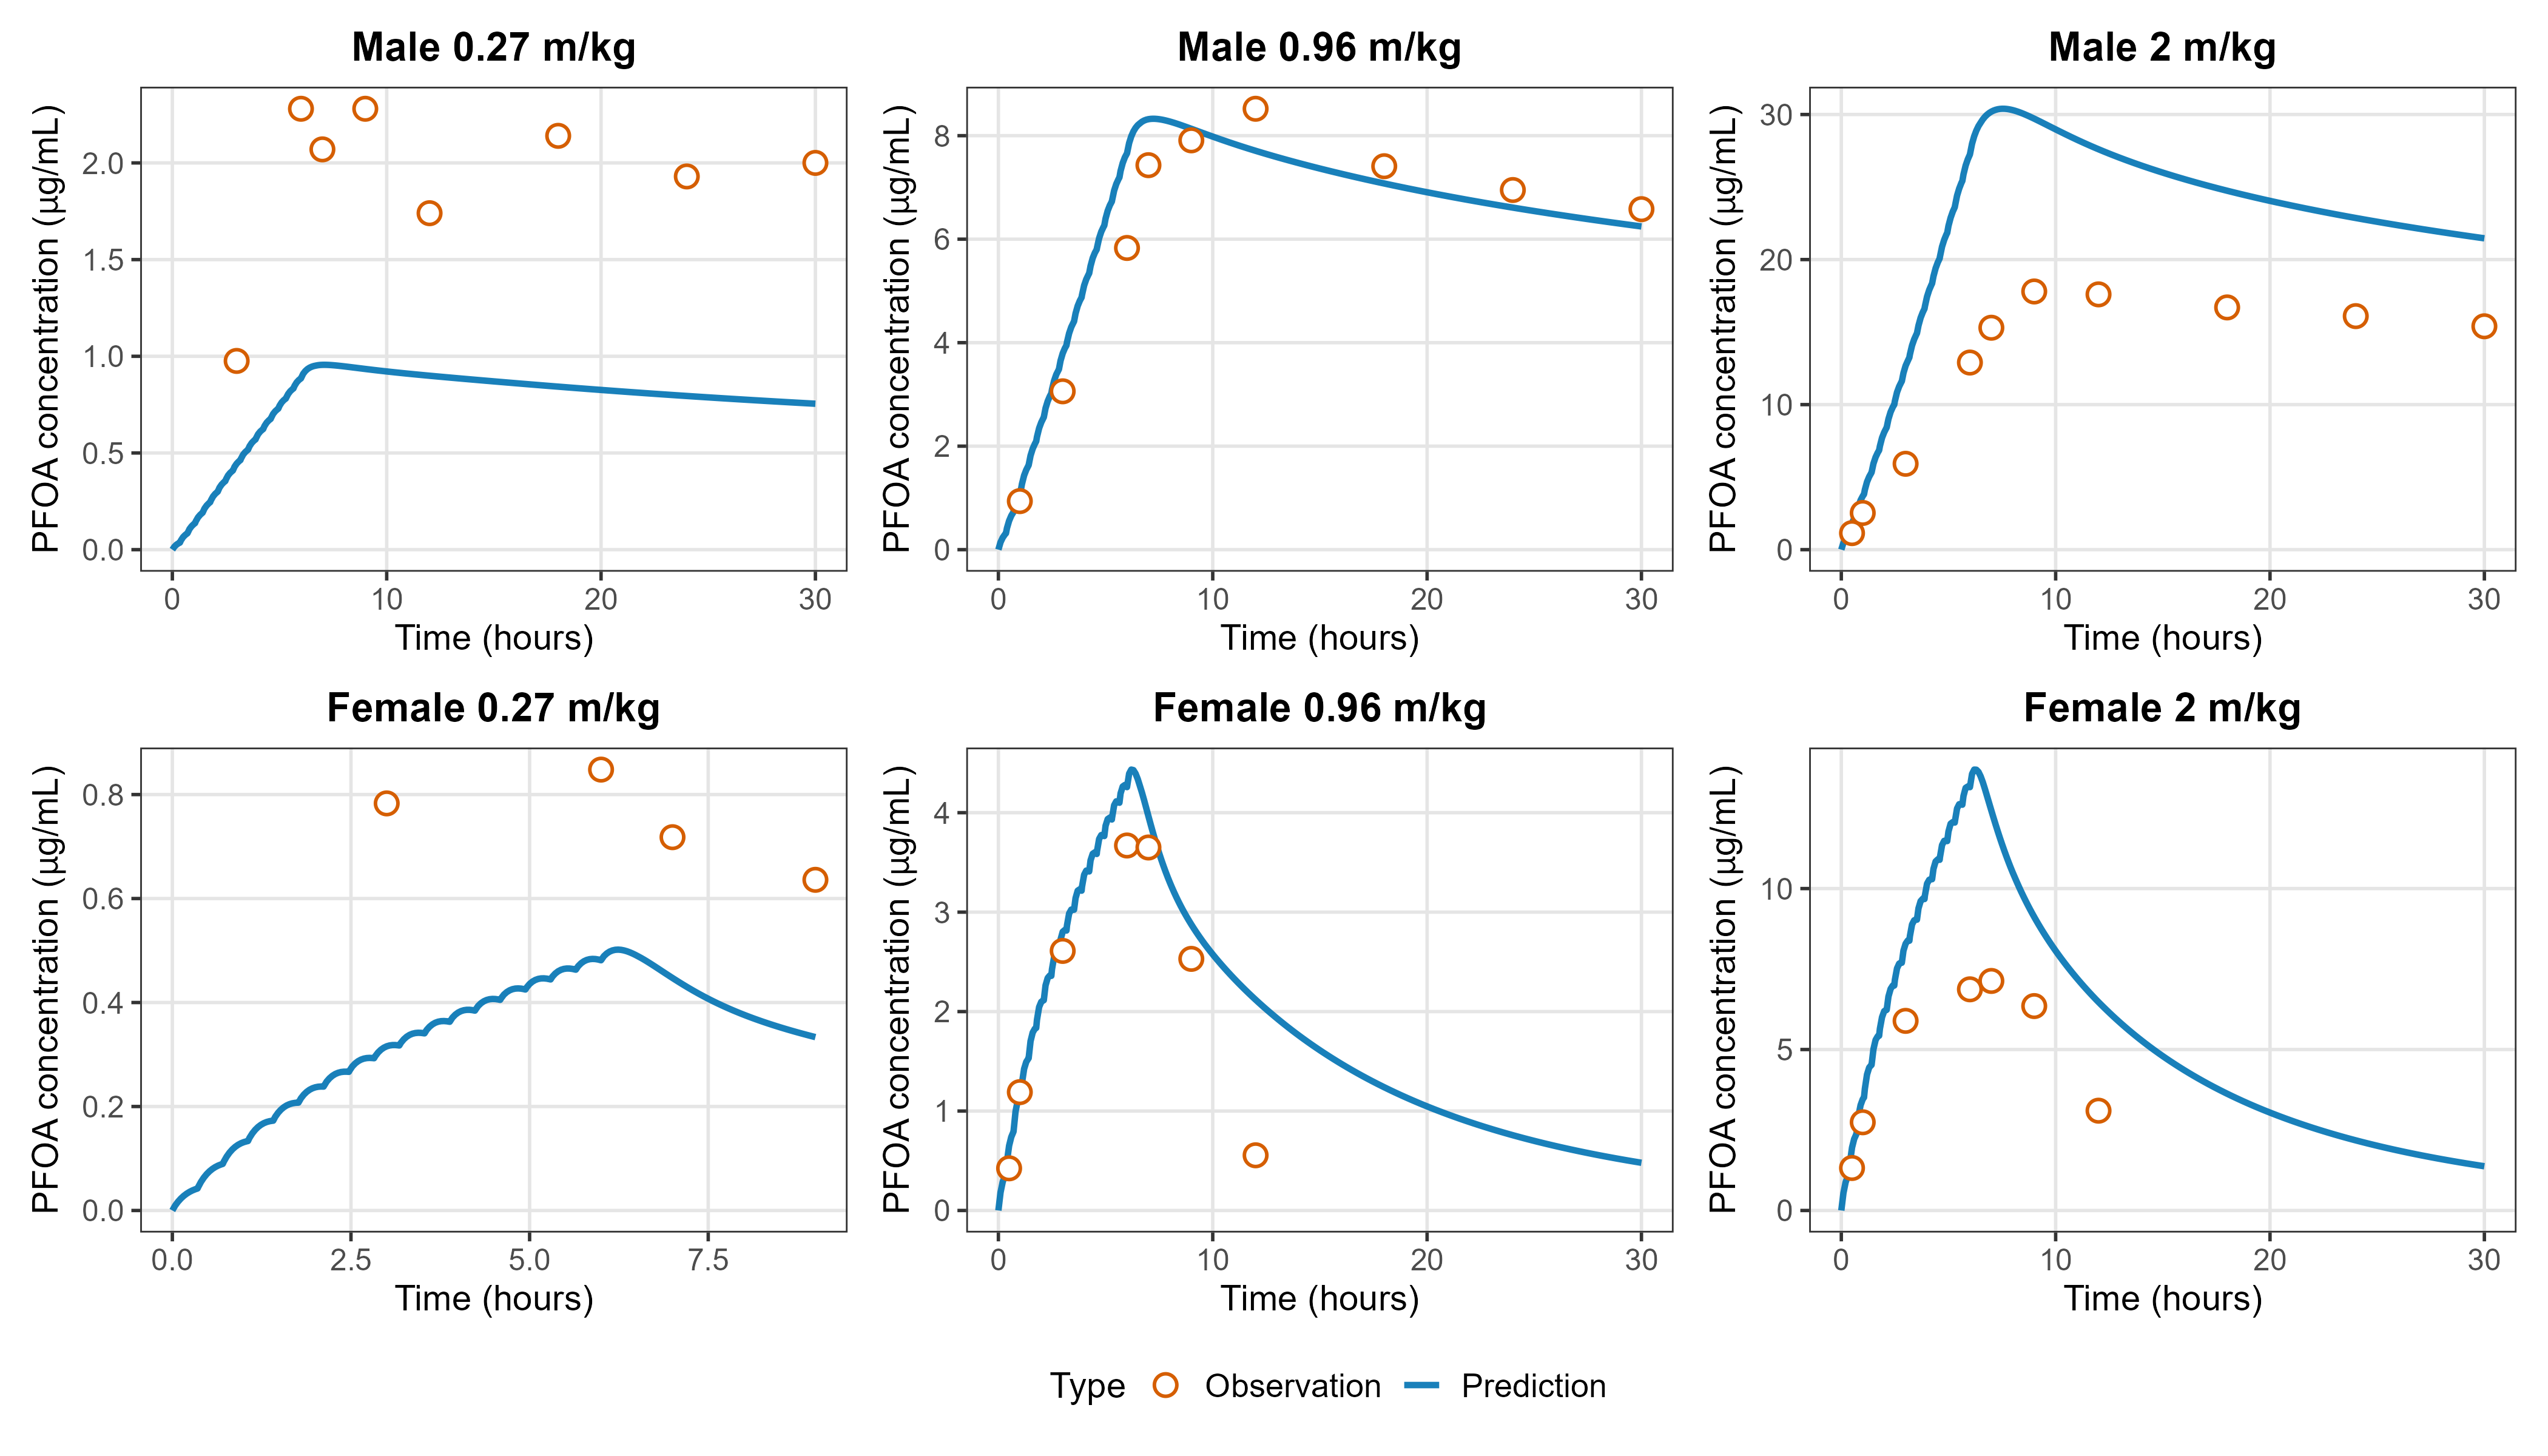
\includegraphics[width=1.0\textwidth]{sup_figures/experiment15.png}
    \caption{Model predictions versus observed plasma concentrations following nasal inhalation in male and female rats. Applied doses were 0.27, 0.96, 2 $\text{mg}/\text{kg}$. Experimental data were obtained from \citet{hinderliter_2006}.The average prediction AAFE was 1.65.}
    \label{fig:experiment15}
\end{figure}


Table \ref{Table:sup_calibration_aafe} presents the detailed AAFE scores for each study used in parameter calibration. In this table, the compartment, along with sex and administration time, is explicitly stated. Specifically, serum, tissues, and excreta are reported separately, because single-point estimates were provided for tissues, while more detailed concentration-time profiles were available for the plasma and excreta compartments. Thus, a distinction is made to account for the different number of samples reported for each compartment.

\begin{table}[H]
\centering
\caption{Goodness-of-fit of the PBK model on the studies used for parameter calibration, expressed through AAFE.}
\label{Table:sup_calibration_aafe}
\resizebox{\textwidth}{!}{
\begin{tabular}{lllcr}
\toprule
\textbf{Study} &   \textbf{Exposure Route}  &   \textbf{Compartment}  & \textbf{Sex} & \textbf{AAFE} \\
\midrule
\citep{dzierlenga_2020}  & iv & plasma & M & 2.33\\
 &iv & plasma & F & 2.05\\
 & oral & plasma & M & 2.87\\
 & oral & plasma & F & 3.01\\
&  oral & tissues & M & 2.27\\
 &  oral & tissues & F & 4.07\\
\citep{gustafsson_2022}  & oral & plasma & M & 1.47\\
 & oral & tissues & M & 5.42\\
&  intratracheal inhalation & plasma & M & 3.06\\
&  intratracheal inhalation & tissues & M & 2.24\\
\citep{hinderliter_2006}  & nose-only inhalation & plasma & M & 1.69\\
&  nose-only inhalation & plasma & F & 1.59\\
\citep{kemper_2003}  & oral & excreta & M & 1.92\\
 & oral & excreta & F & 1.43 \\
\citep{kim_2016}  &  oral & serum & M & 2.33\\
 & oral & serum & F & 2.61\\
 & IV & serum & M & 1.48\\
 & IV & serum & F & 2.31\\
&  oral & tissues & M & 2.13\\
 & oral & tissues & F & 2.59\\
 & IV & tissues & M & 2.19 \\
 & IV & tissues & F & 5.29\\
\citep{kudo_2007}  & IV & tissues & M & 2.36 \\
\midrule
\end{tabular}
}

\raggedright
\footnotesize
\vspace{0.5em}
\raggedright
\scriptsize
AAFE: Absolute Average Fold Error; IV: intravenous; F: female; M: male \\
\end{table}
\newpage

\section{Goodness-of-fit on Validation Data}

The following section presents the goodness-of-fit plots on the \textit{in vivo} data used for model validation. Specifically, model predictions againste obsevations are presented for the studies of \citet{cui_2009}, \citep{cui_2010}, \citep{lupton_2021}, \citep{hinderliter_2006}, and \citet{kemper_2003}.


\begin{figure}[H]
    \centering
    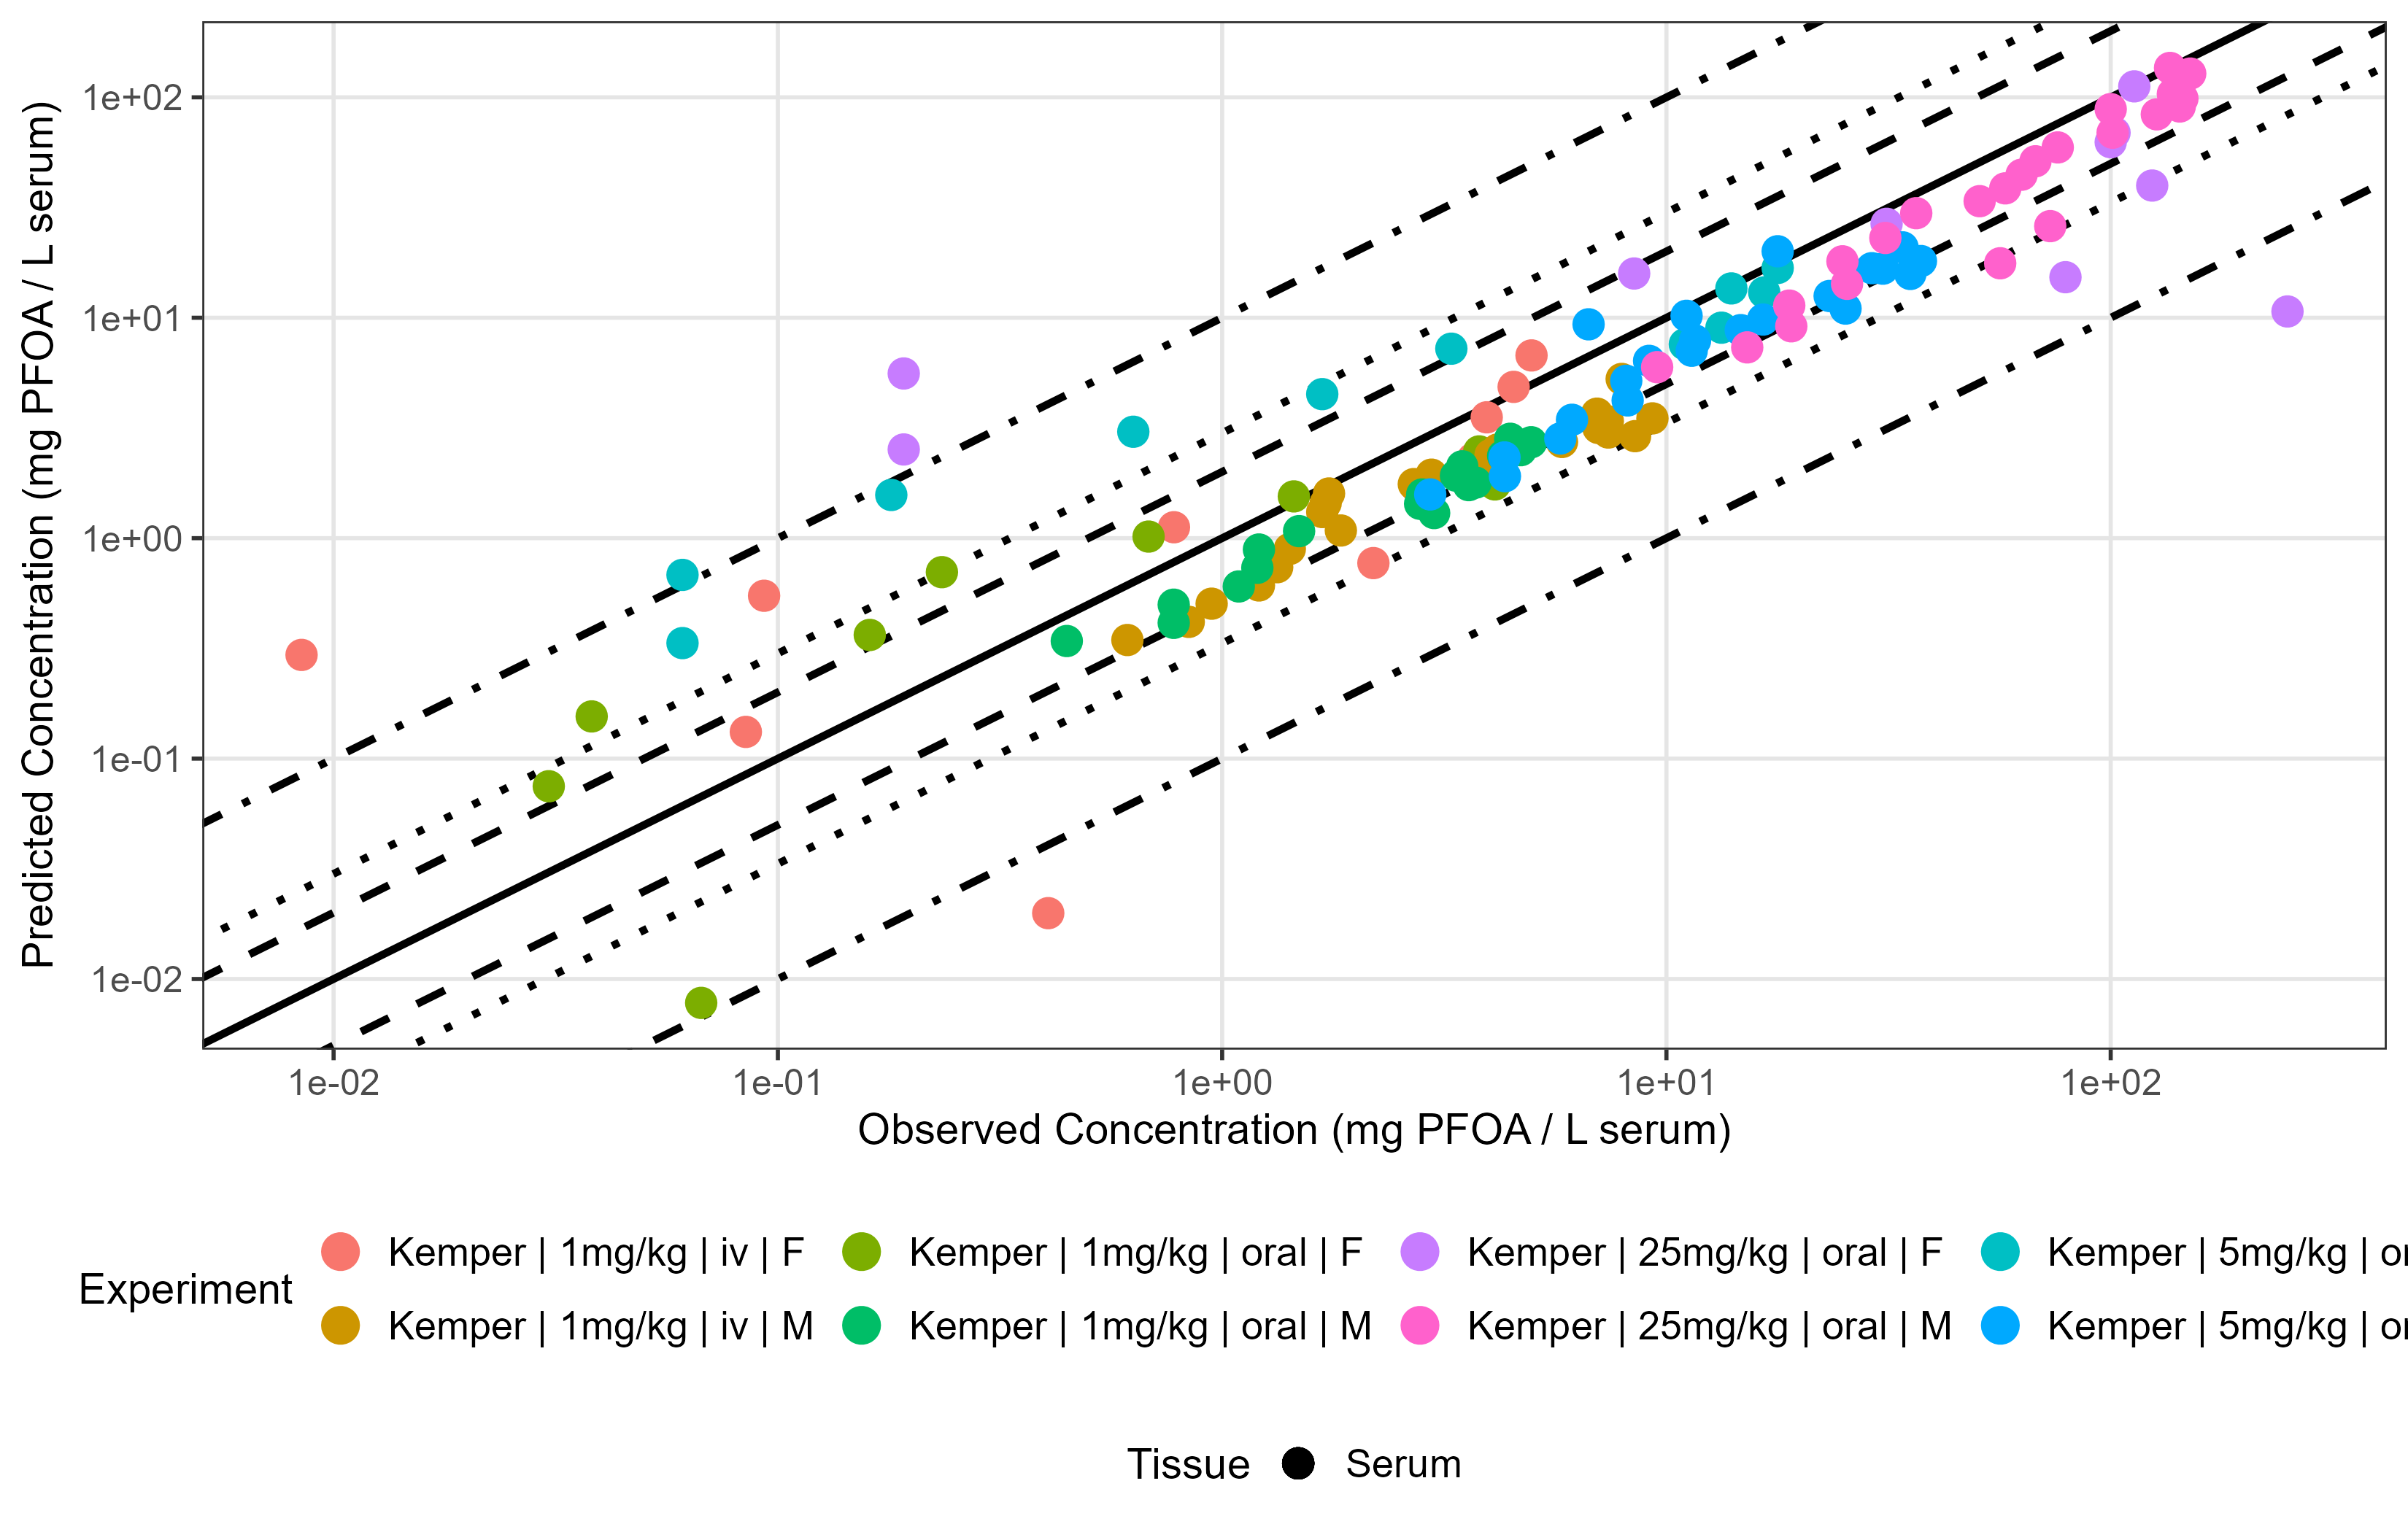
\includegraphics[width=1.0\textwidth]{sup_figures/validation_plot_PFOA_serum.png}
    \caption{Model predictions versus observed serum concentrations following oral or IV administration in male and female rats. Applied doses were 1, 5, 25 $\text{mg}/\text{kg}$. Experimental data were obtained from \citet{kemper_2003}.The average prediction AAFE was 2.02.}
    \label{fig:validation_serum}
\end{figure}



\begin{figure}[H]
    \centering
    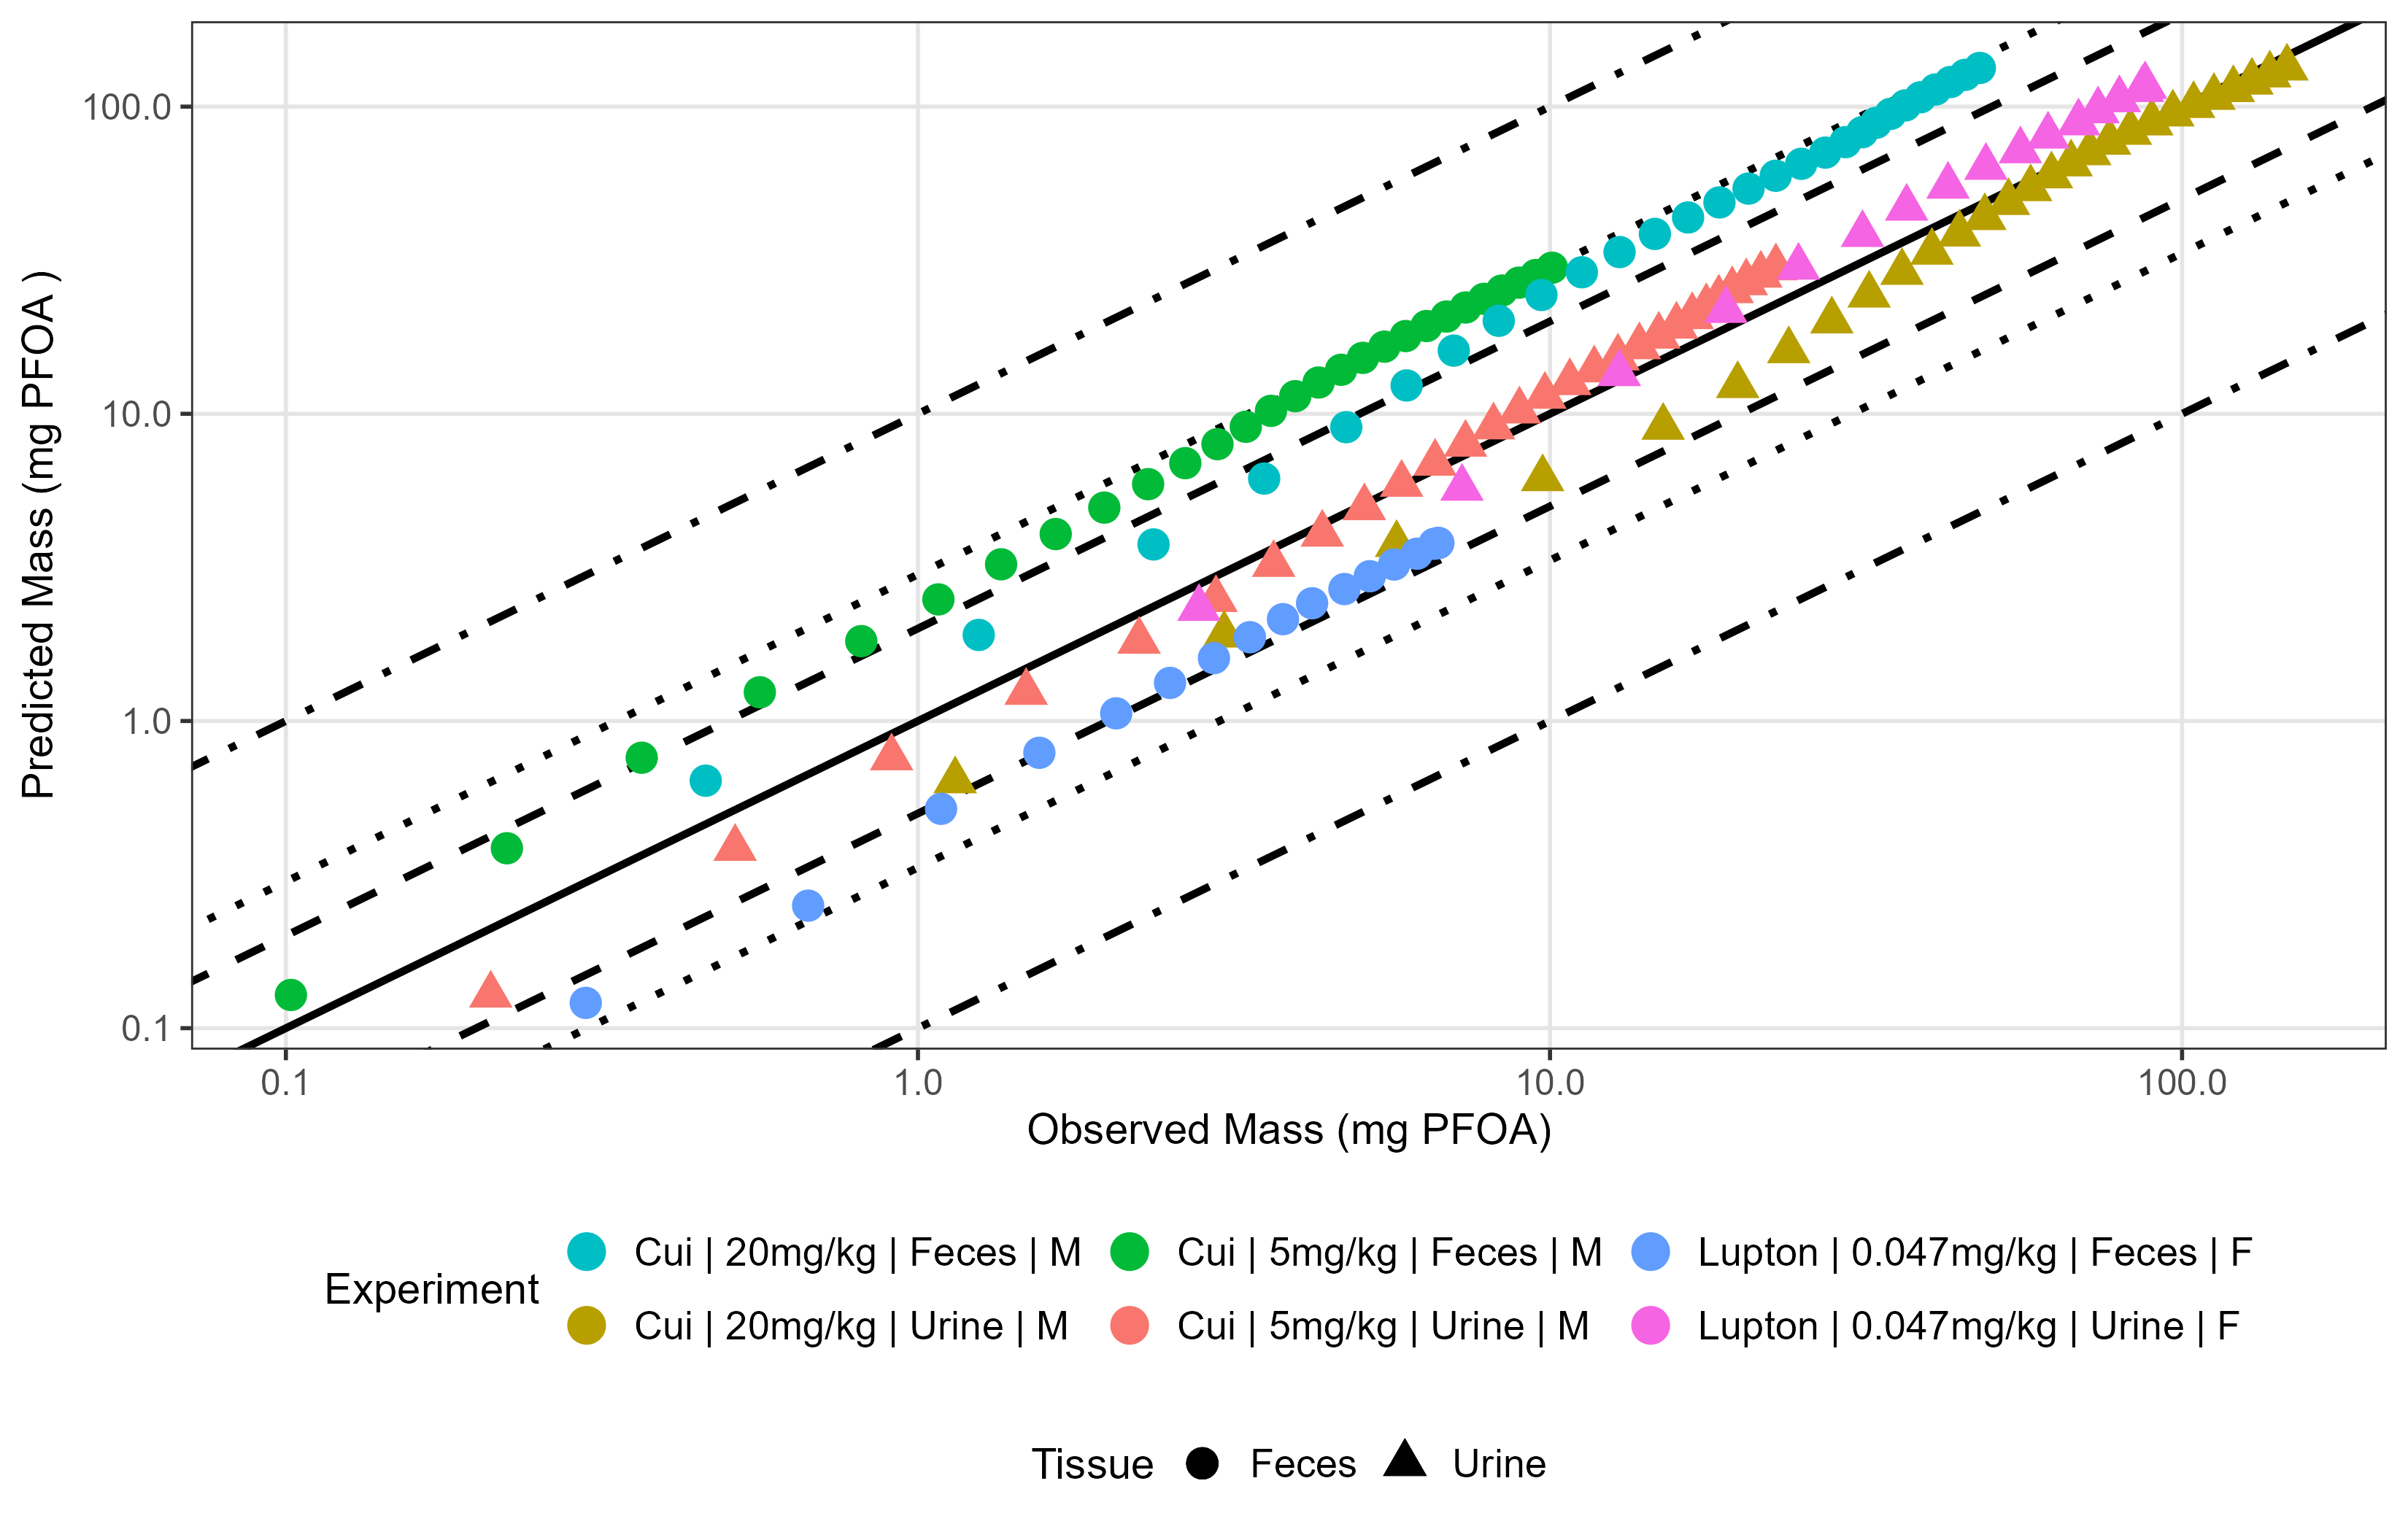
\includegraphics[width=1.0\textwidth]{sup_figures/validation_plot_PFOA_excreta.png}
    \caption{Model predictions versus observed excreta masses following repeated oral administration in male and female rats. Applied doses were 0.047 $\text{mg}/\text{kg}/\text{day}$ in female rats for repeated administration of 13 days \citep{lupton_2021}, 5 and 10 $\text{mg}/\text{kg}/\text{day}$ in male rats for repeated administration of 28 days \citep{cui_2009,cui_2010} The average prediction AAFE was 1.69.}
    \label{fig:validation_excreta}
\end{figure}


\begin{figure}[H]
    \centering
    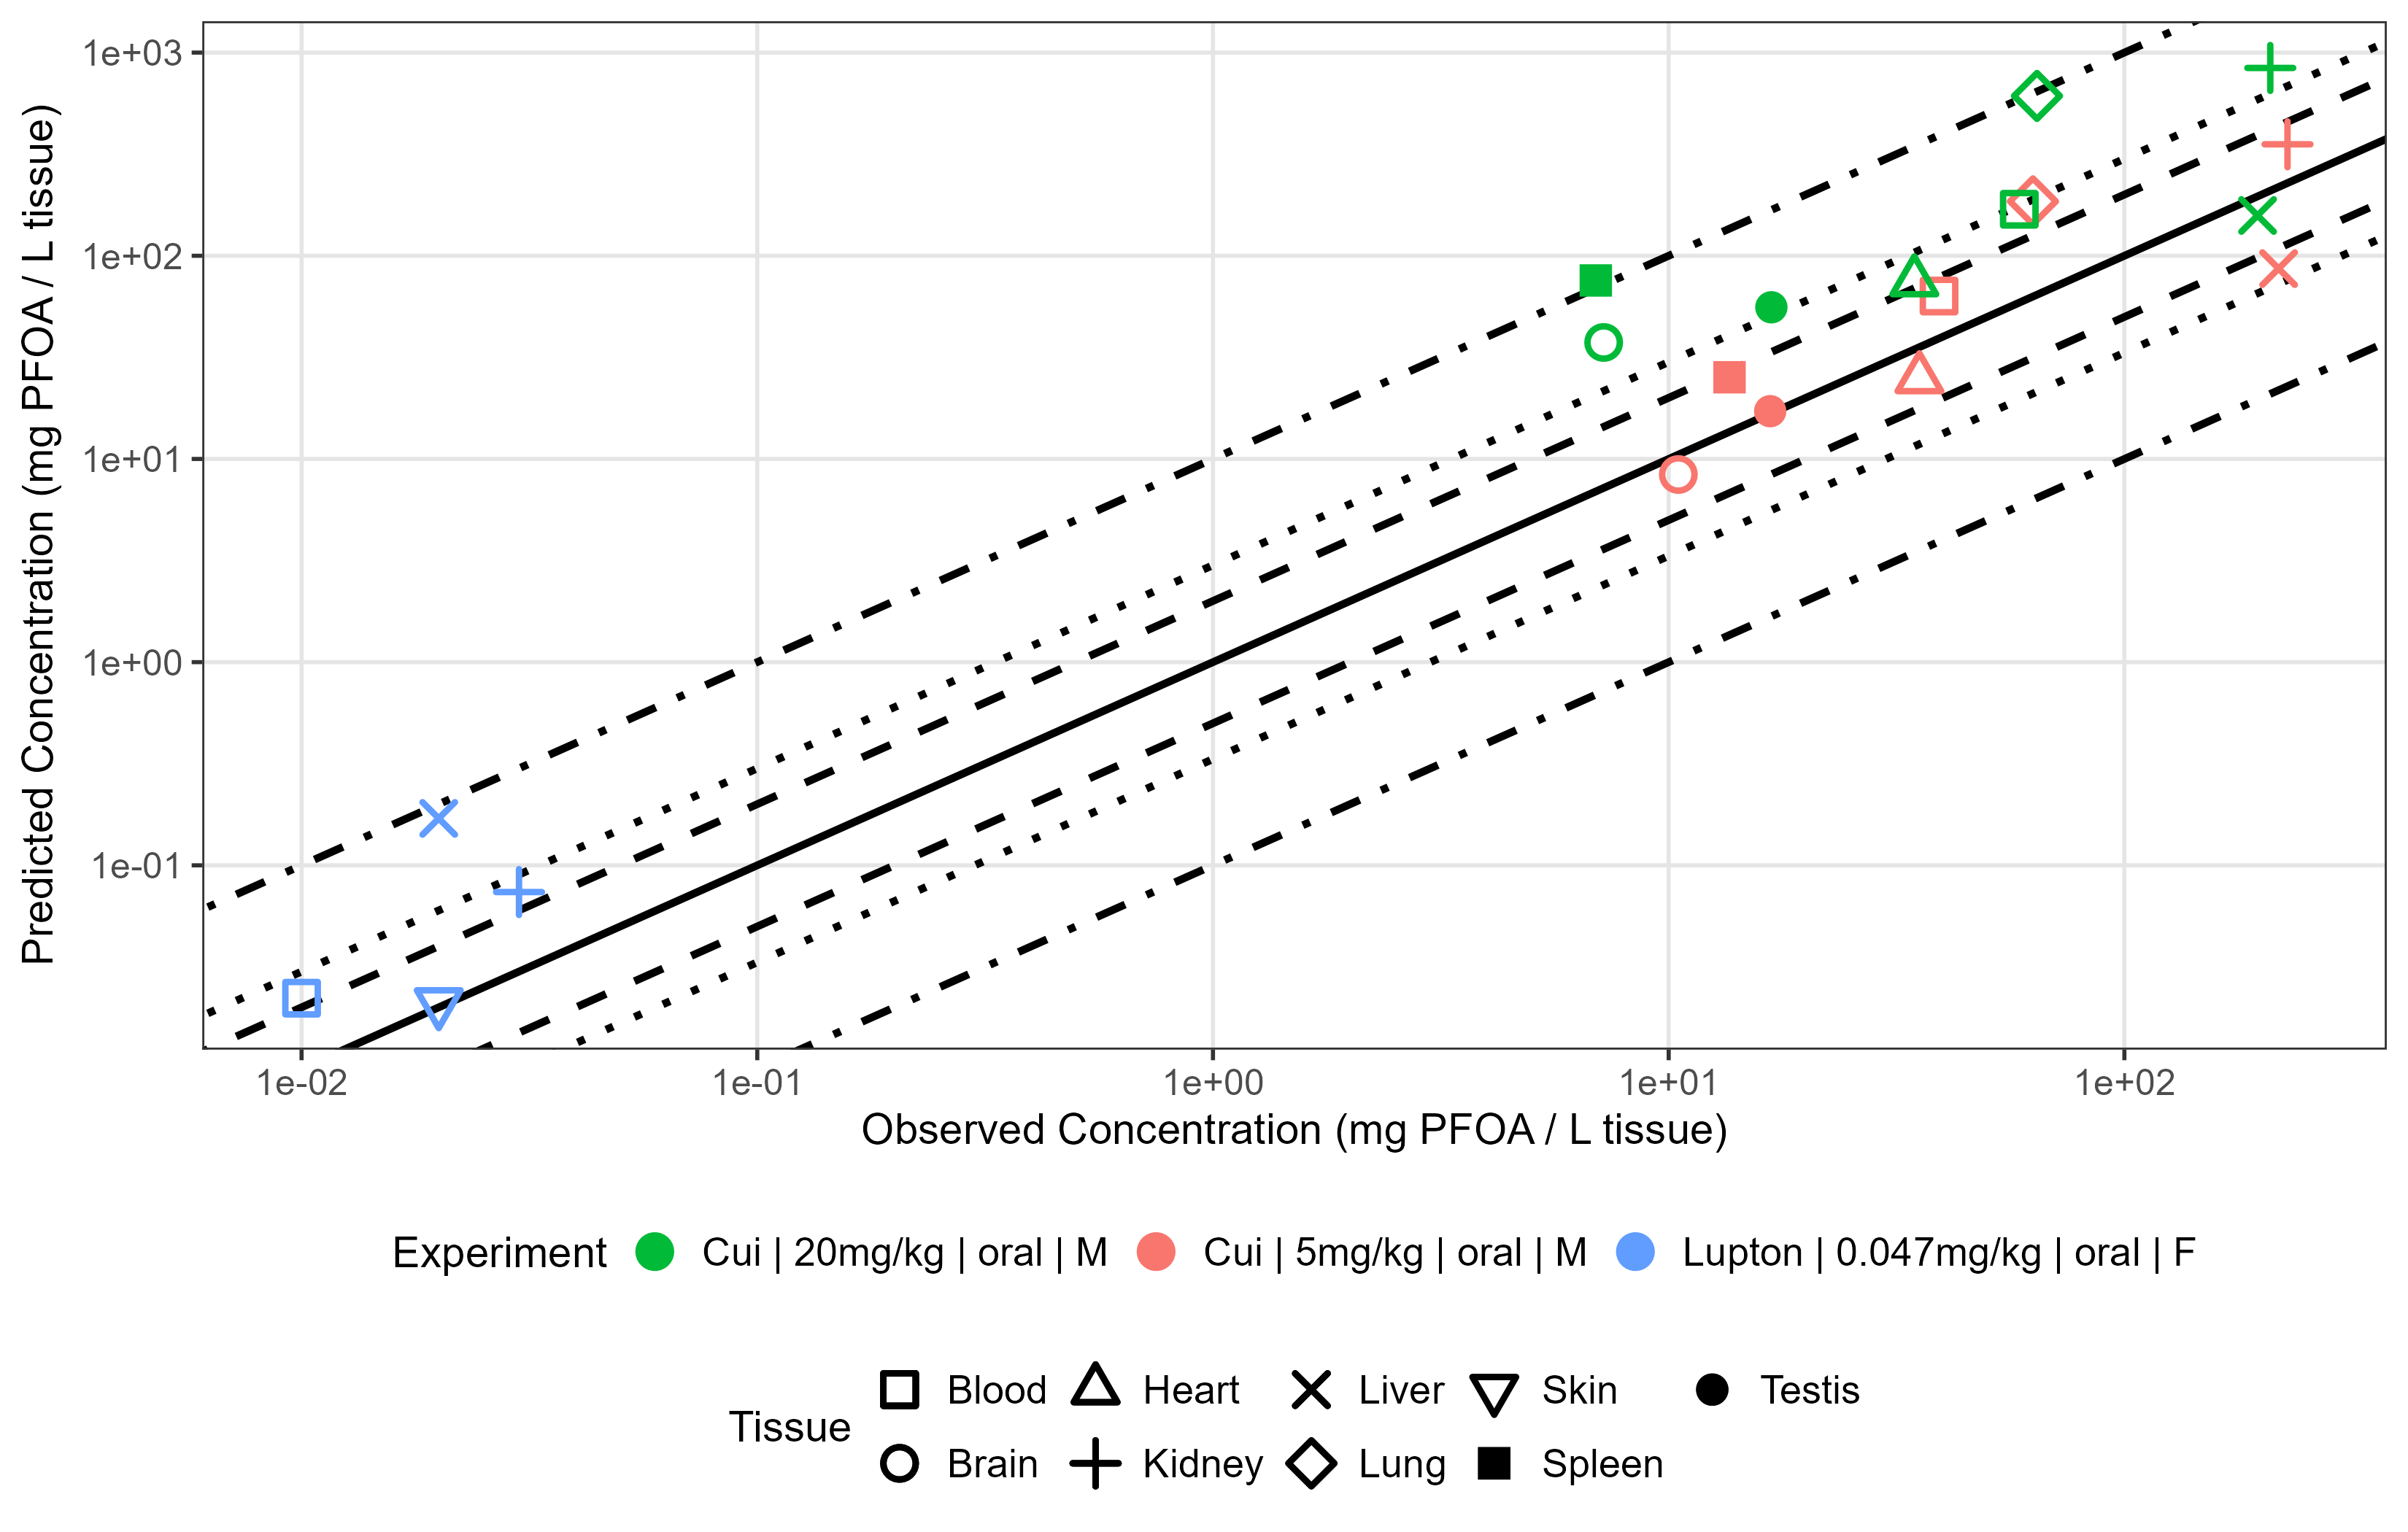
\includegraphics[width=1.0\textwidth]{sup_figures/validation_plot_PFOA_tissues.png}
    \caption{Model predictions versus observed tissue concentration following repeated oral administration in male and female rats. Applied doses were 0.047 $\text{mg}/\text{kg}/\text{day}$ in female rats for repeated administration of 13 days \citep{lupton_2021}, 5 and 20 $\text{mg}/\text{kg}/\text{day}$ in male rats for repeated administration of 28 days \citep{cui_2009,cui_2010}. The average prediction AAFE was 2.58.}
    \label{fig:validation_tissues}
\end{figure}

\begin{figure}[H]
    \centering
    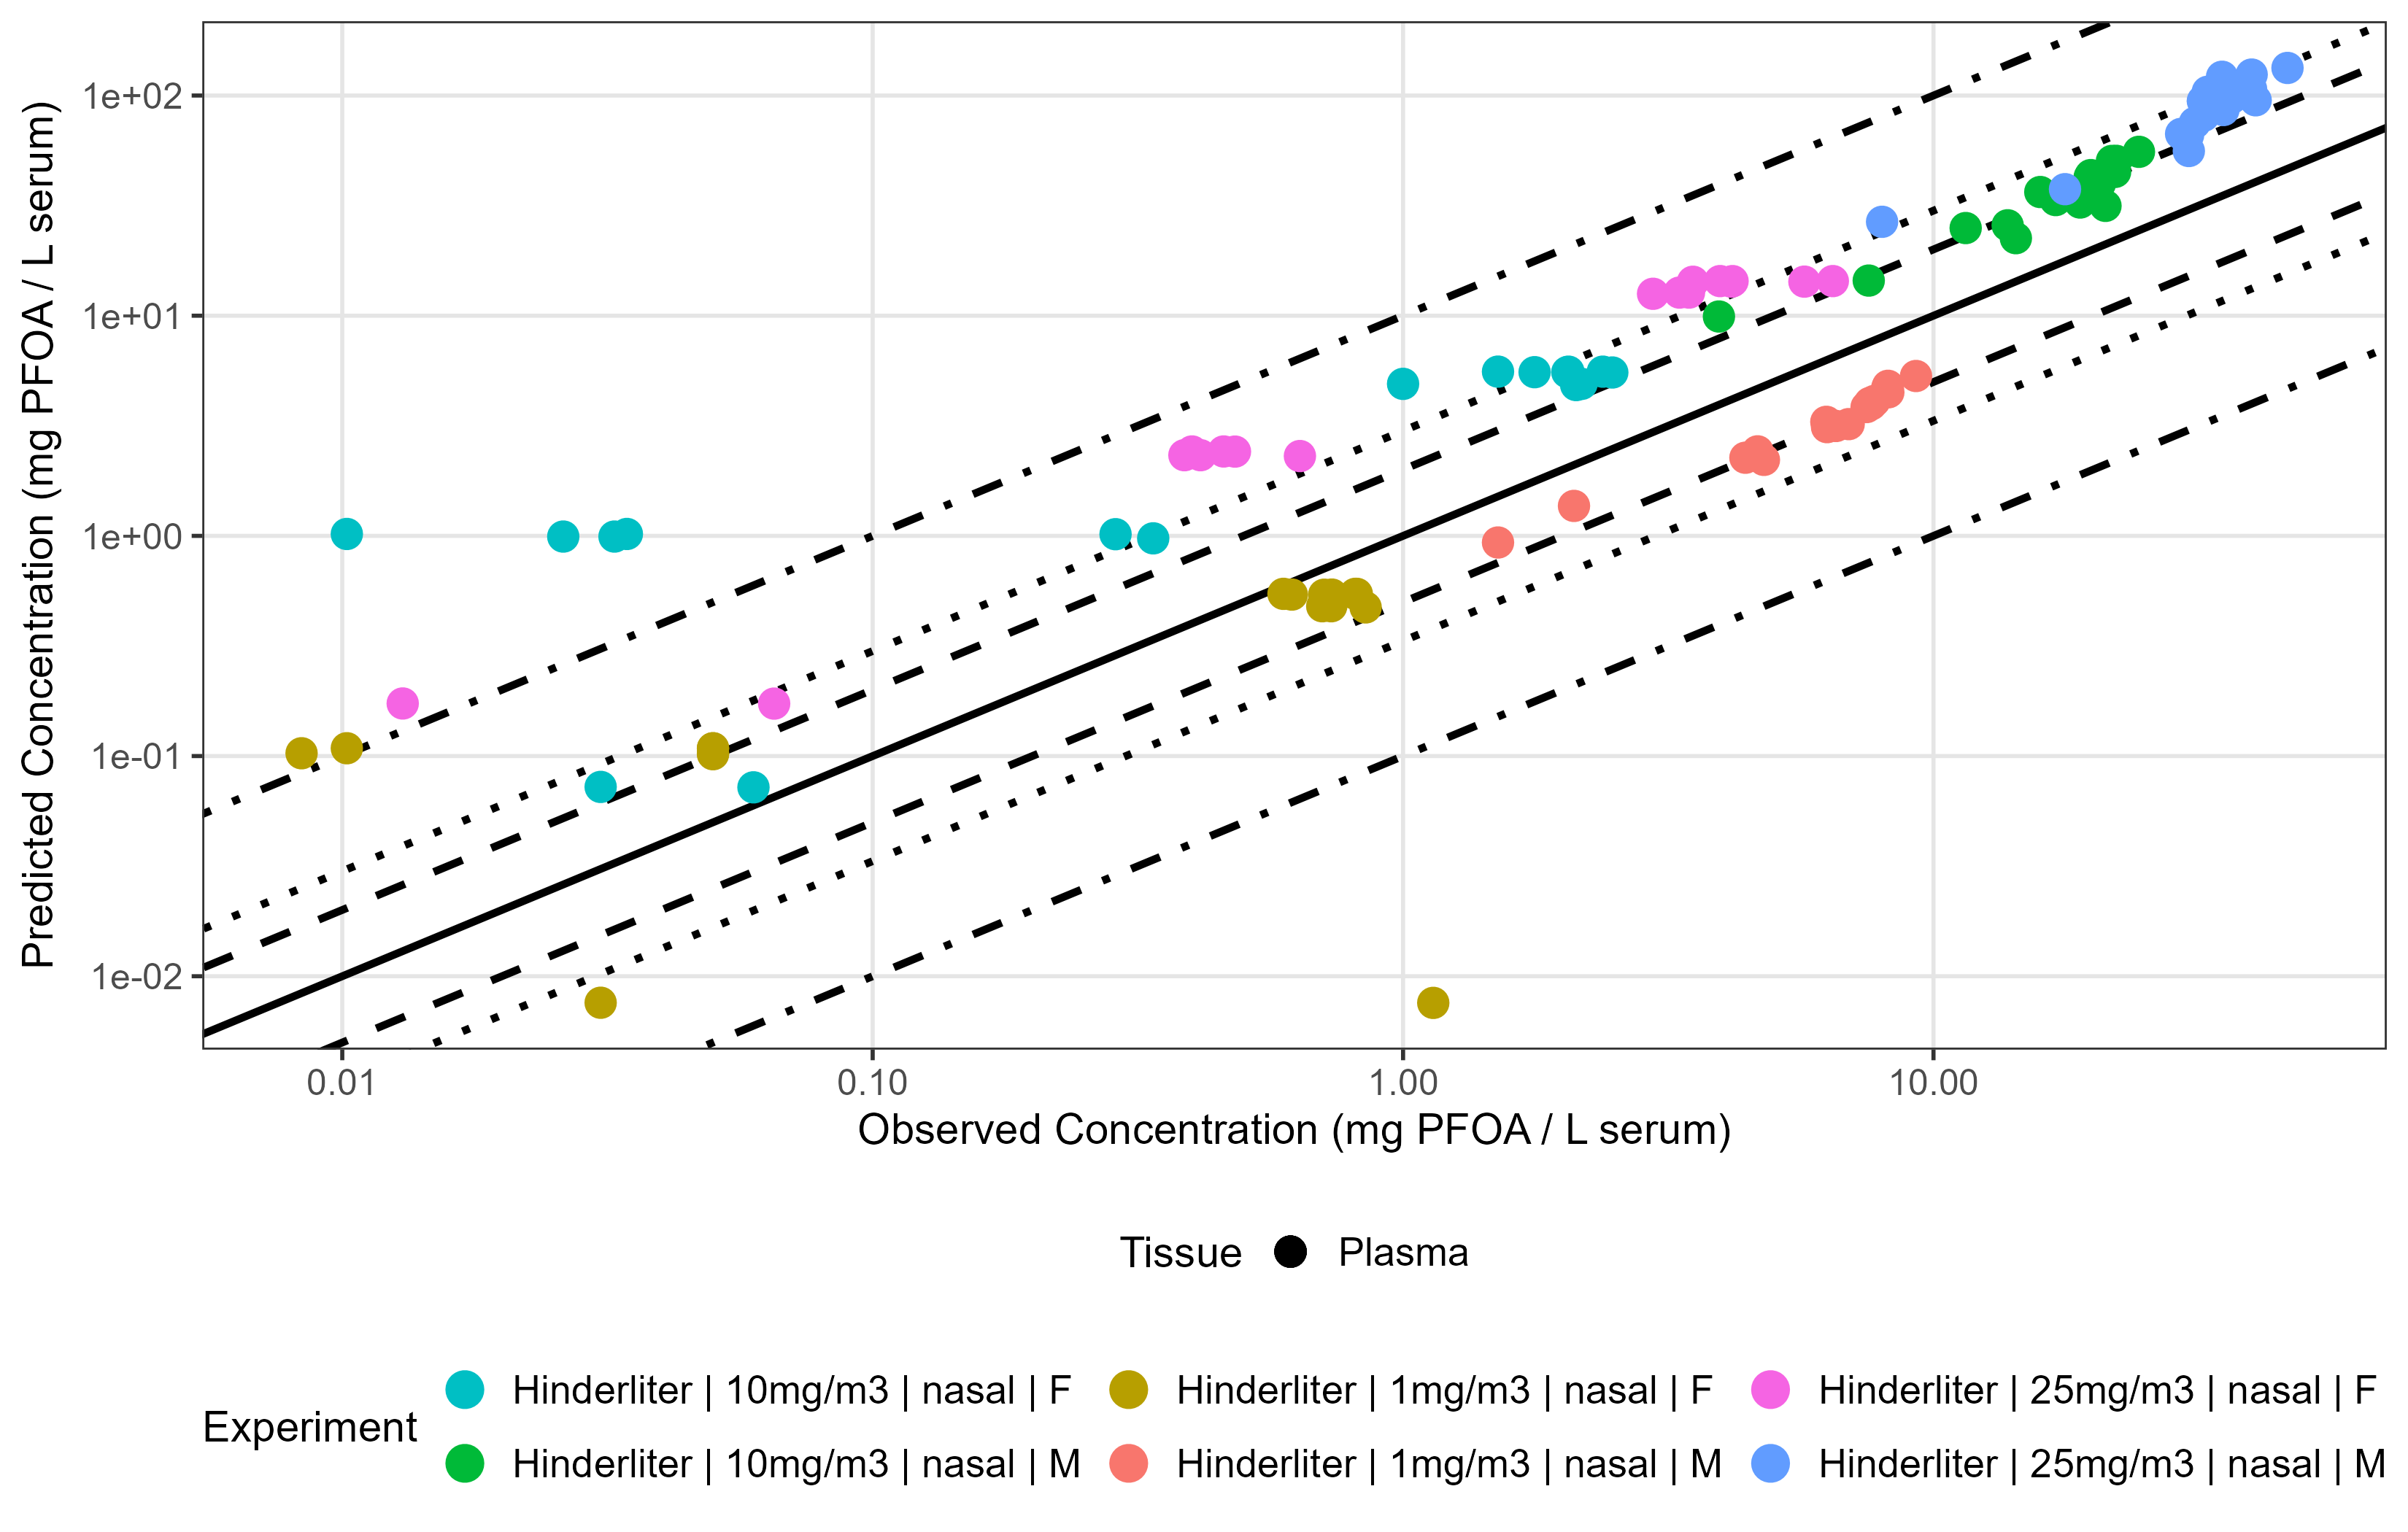
\includegraphics[width=1.0\textwidth]{sup_figures/validation_plot_PFOA_nasal_serum.png}
    \caption{Model predictions versus observed plasma concentration following repeated nasal inhalation administration in male and female rats. Applied concentrations were 1, 10 and 25 $\text{mg}/\text{m}^3$ for 6 h per day, 5 days per week for 3 weeks\citep{hinderliter_2006}. The average prediction AAFE was 2.90.}
    \label{fig:validation_nasal}
\end{figure}

\begin{table}[H]
\centering
\caption{Predictive performance of the PBK model on the studies used for validation, expressed through AAFE.}
\label{Table:sup_validation_aafe}
\resizebox{\textwidth}{!}{
\begin{tabular}{lllcr}
\toprule
\textbf{Study} &   \textbf{Exposure Route}  &   \textbf{Compartment}  & \textbf{Sex} & \textbf{AAFE} \\
\midrule
\citep{cui_2009}  & repeated oral & tissues & M & 2.57\\
 \citep{cui_2010}  & repeated oral & excreta & M & 1.74\\
\citep{lupton_2021}  & repeated oral & tissues & F & 2.64\\
 & repeated oral & excreta & F & 1.54\\
\citep{hinderliter_2006}  & repeated nose-only inhalation & plasma & M & 2.15\\
&  repeated nose-only inhalation & plasma & F & 3.09\\
\citep{kemper_2003}  & oral & serum & M & 1.80\\
 & oral & serum & F & 2.87 \\
 & IV & serum & M &1.66 \\
 & IV & serum & F & 2.94\\

\midrule
\end{tabular}
}

\raggedright
\footnotesize
\vspace{0.5em}
\raggedright
\scriptsize
AAFE: Absolute Average Fold Error; IV: intravenous; F: female; M: male \\
\end{table}

\section{PBK Model Simulations and Scenario Analyses}

This section uses the developed PBK model both to illustrate the biodistribution of PFOA and to explore selected what-if scenarios. Figure \ref{fig:localisation} illustrates the free and bound concentrations of PFOA across the subcompartments of the liver, kidney, lung, and brain. Marked differences in distribution patterns are observed between organs: the liver shows the highest bound PFOA concentration in the intracellular space, in the kidney and lung the intracellular free PFOA concentration is dominant, and, as expected, the brain exhibits the highest concentrations in the blood, since the blood-brain barrier does not permit easy entrance of PFOA in the tissue space.Figure \ref{fig:kidney_compartments} depicts PFOA localisation across the subcompartments of the renal tubule. In both male and female rats, concentrations in the proximal tubule cells overwhelmingly exceed those in all other compartments. Moreover, concentrations within the renal tubule increase progressively from the initial to the terminal segment over the examined time span. The impact of the physiological flow reduction along the renal tubule is illustrated in Figure \ref{fig:flow_drop}. Without this reduction, the model fails to reproduce the observed serum concentrations. This discrepancy arises because, in the absence of a flow drop, renal content moves too rapidly relative to diffusion across the tubule walls, which mediates reabsorption of PFOA in addition to the active transport occurring in the proximal tubule.

\begin{figure}[H]
    \centering
    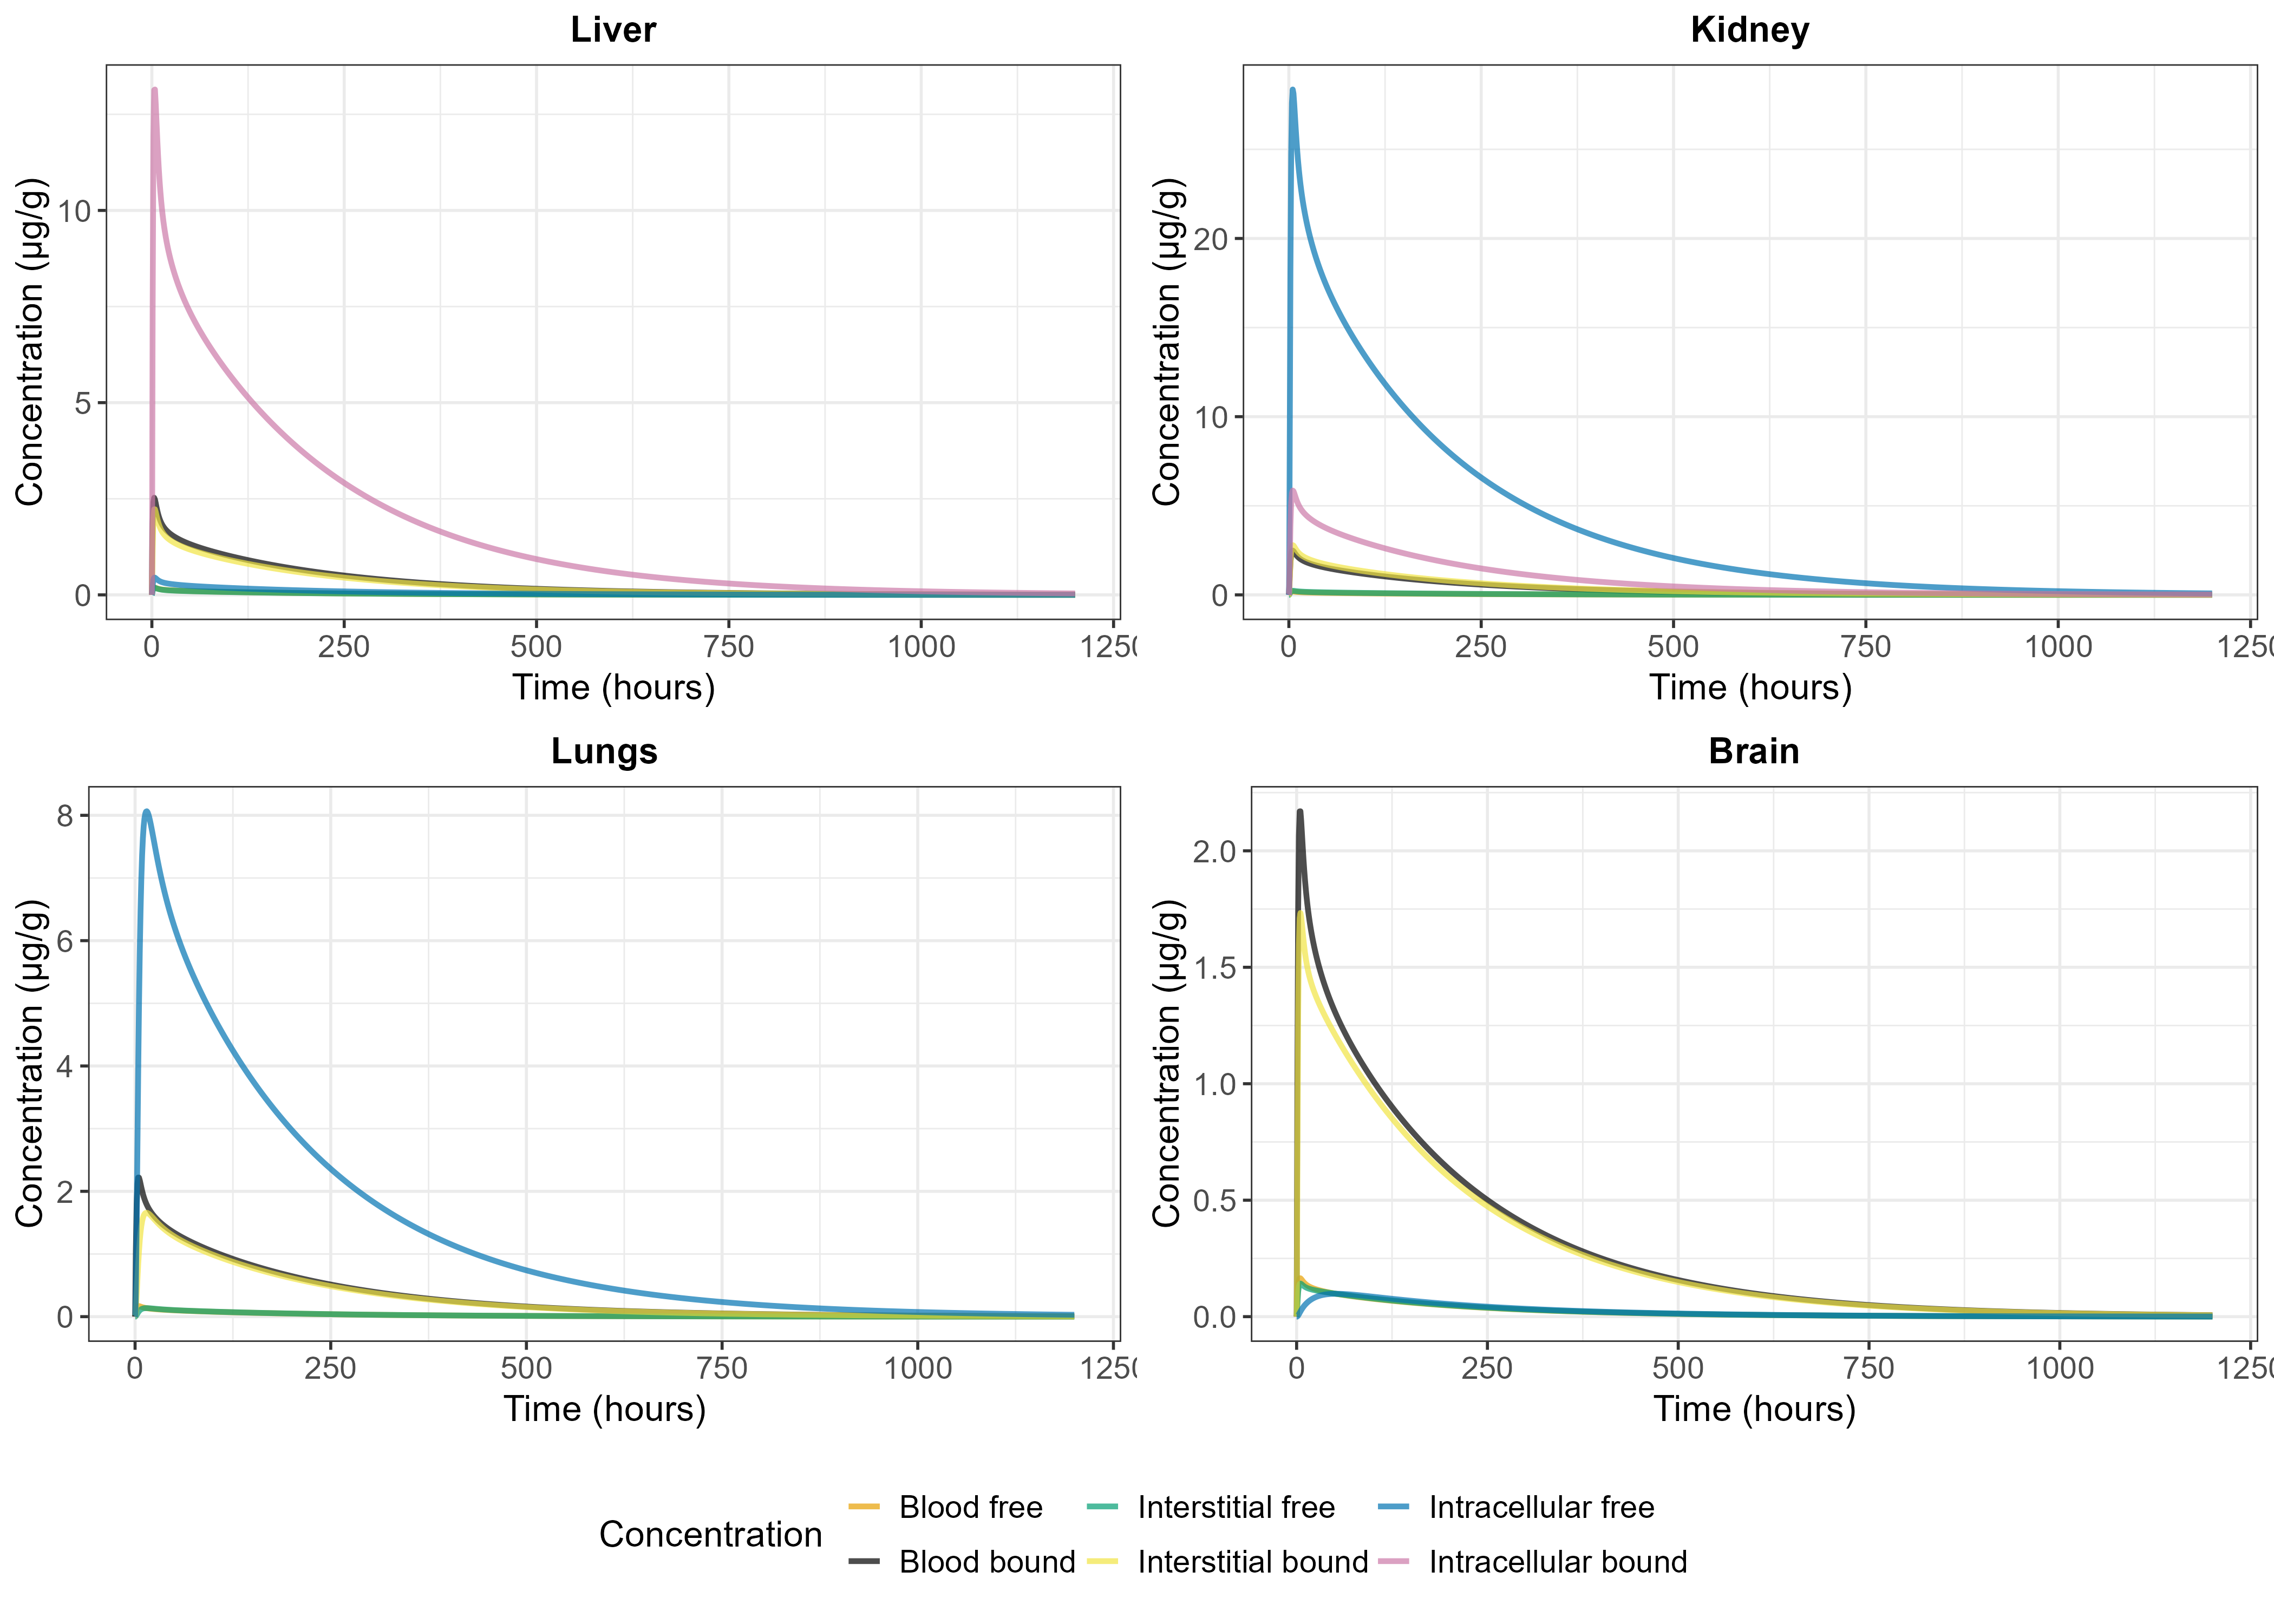
\includegraphics[width=1.0\textwidth]{sup_figures/organ_localisation_plots.png}
    \caption{PFOA free and bound concentrations in blood, interstitial and intracellular space in the liver, kidney, lung and brain. Simulations describe the biodistribution in 300 g male rats after oral administration of 1 mg/kg.}
    \label{fig:localisation}
\end{figure}


\begin{figure}[H]
    \centering
    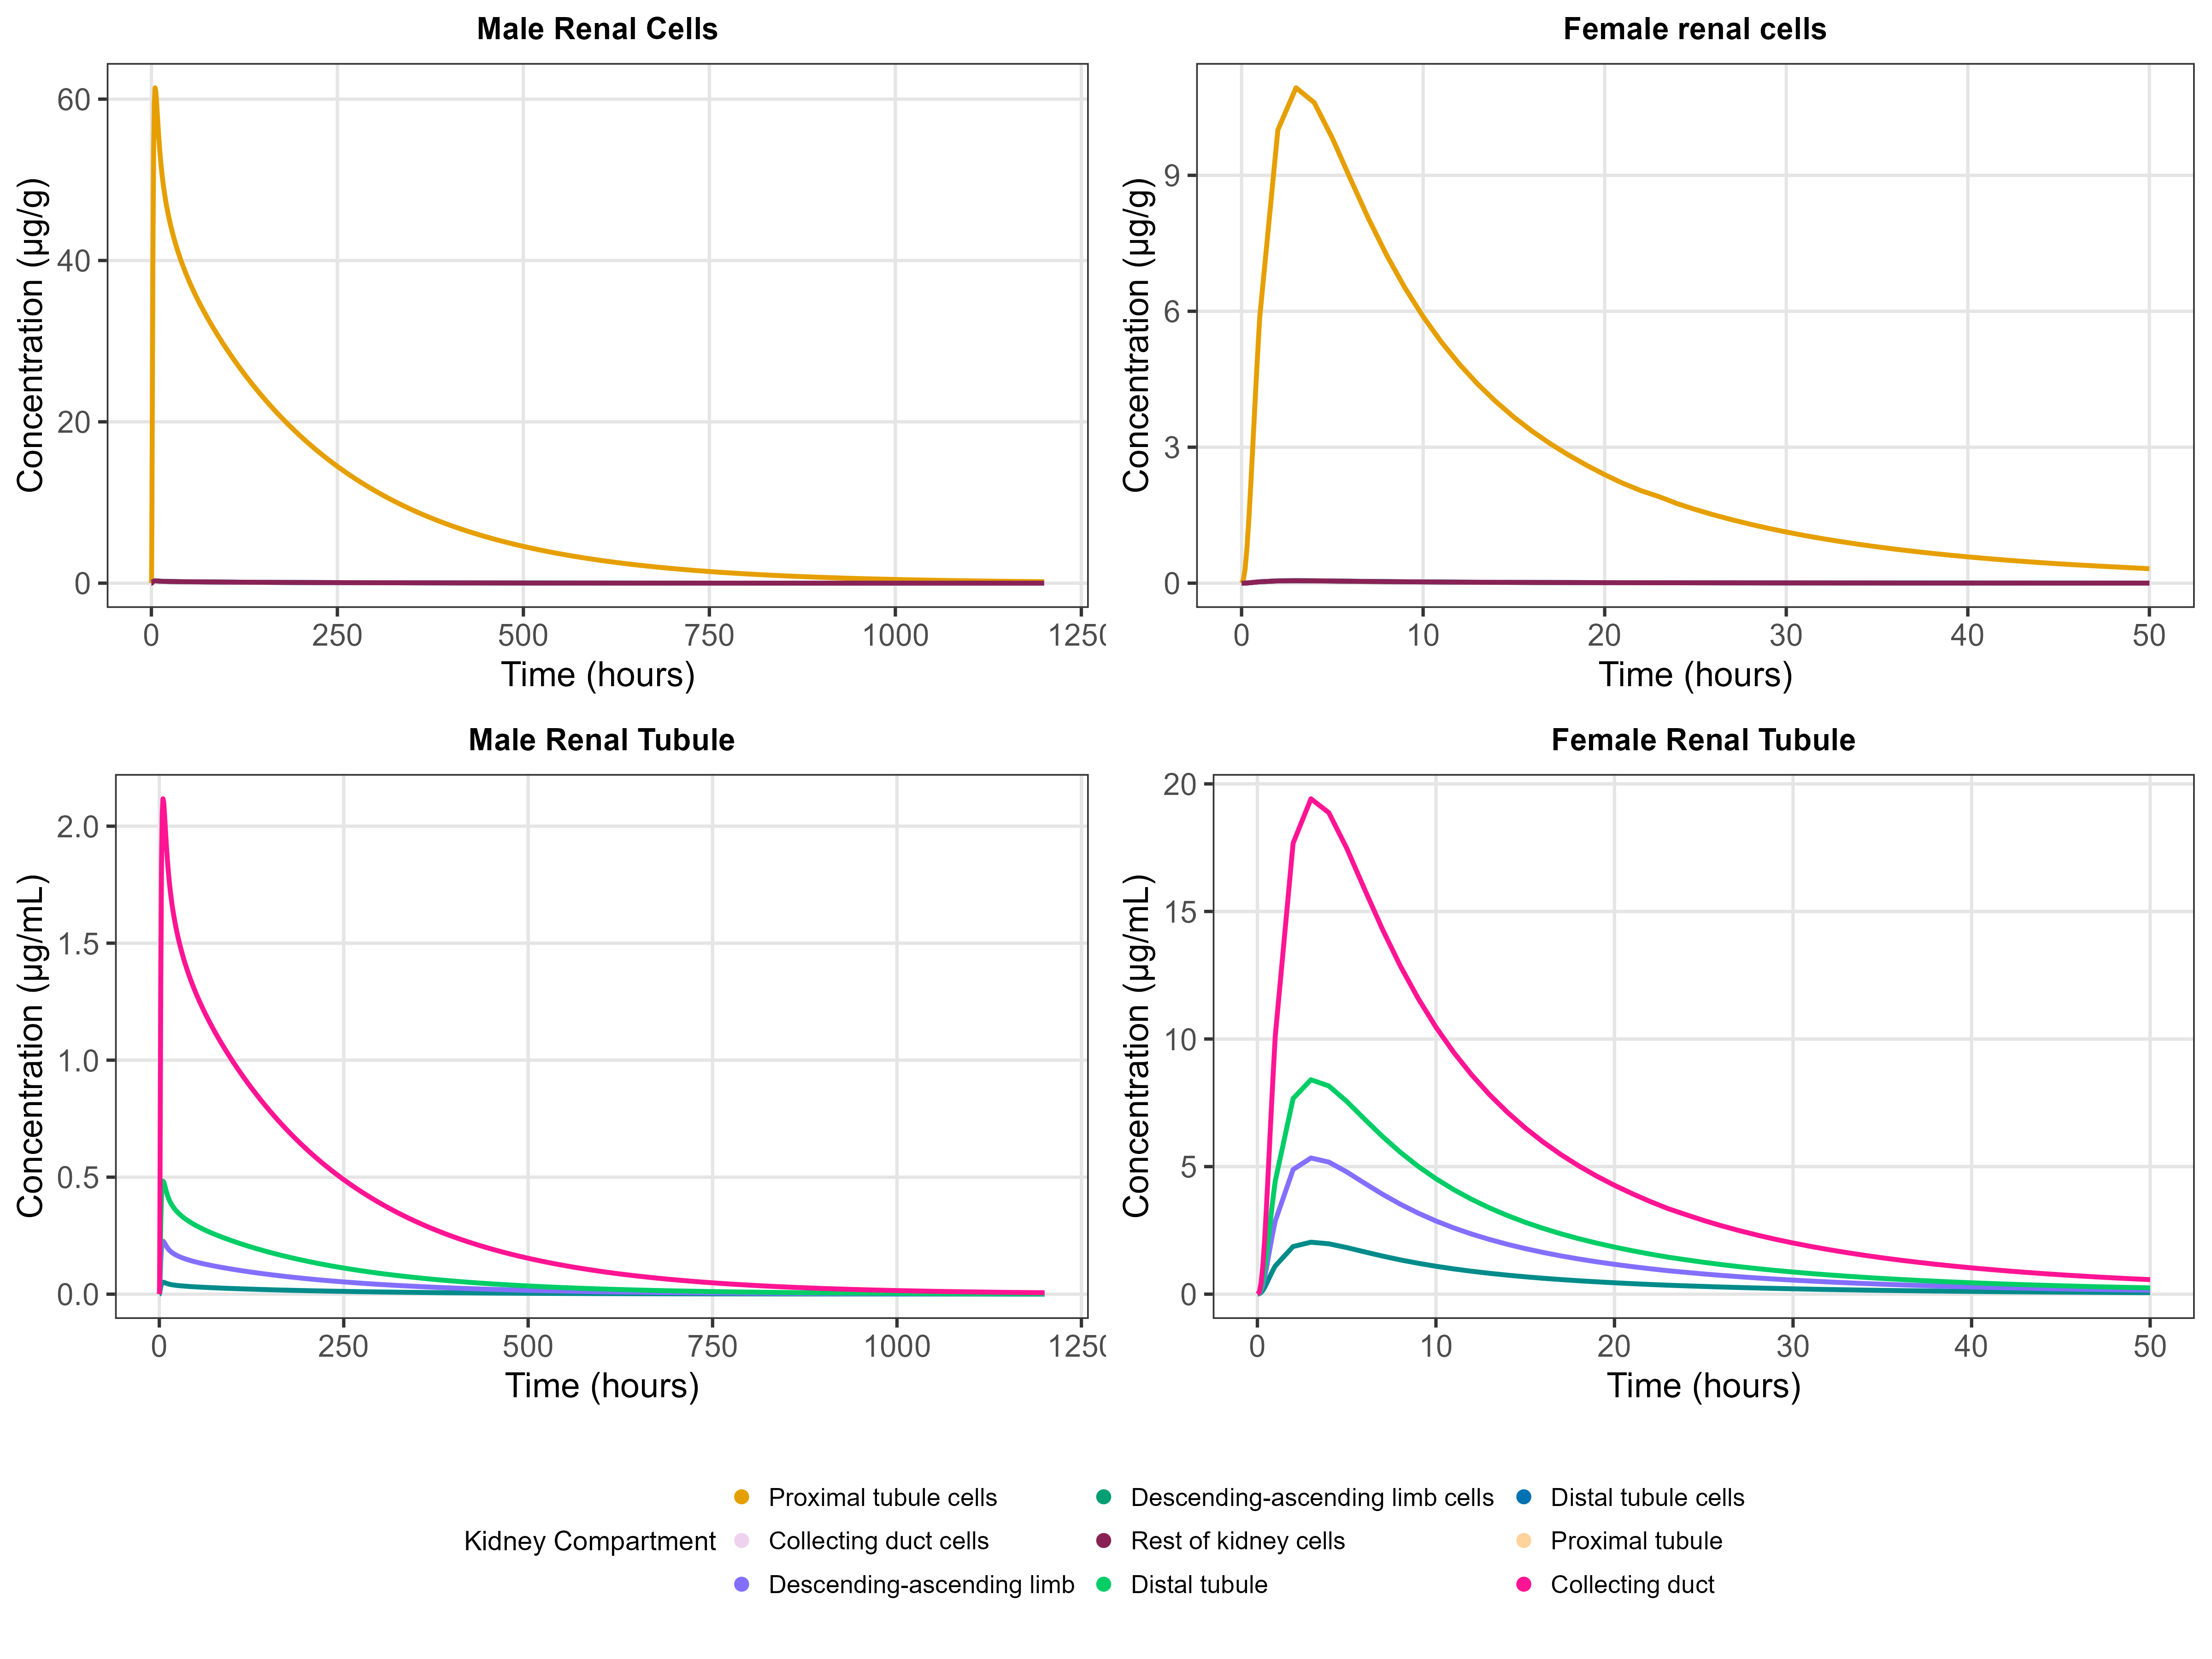
\includegraphics[width=1.0\textwidth]{sup_figures/kidney_compartments_plot.png}
    \caption{PFOA concentration in the kidney subcompartments: in renal tubule cells (top row), including proximal tubule cells, descending-ascending limb cells, distal tubule cells and collecting duct cells, as well as renal tubule (bottom row), including proximal tubule, descending-ascending limb, distal tubule and collecting duct. Simulations describe the result of orally administering 1 mg/kg PFOA to 300 g male (left column) or 200 g female (right column) rats.}
    \label{fig:kidney_compartments}
\end{figure}


\begin{figure}[H]
    \centering
    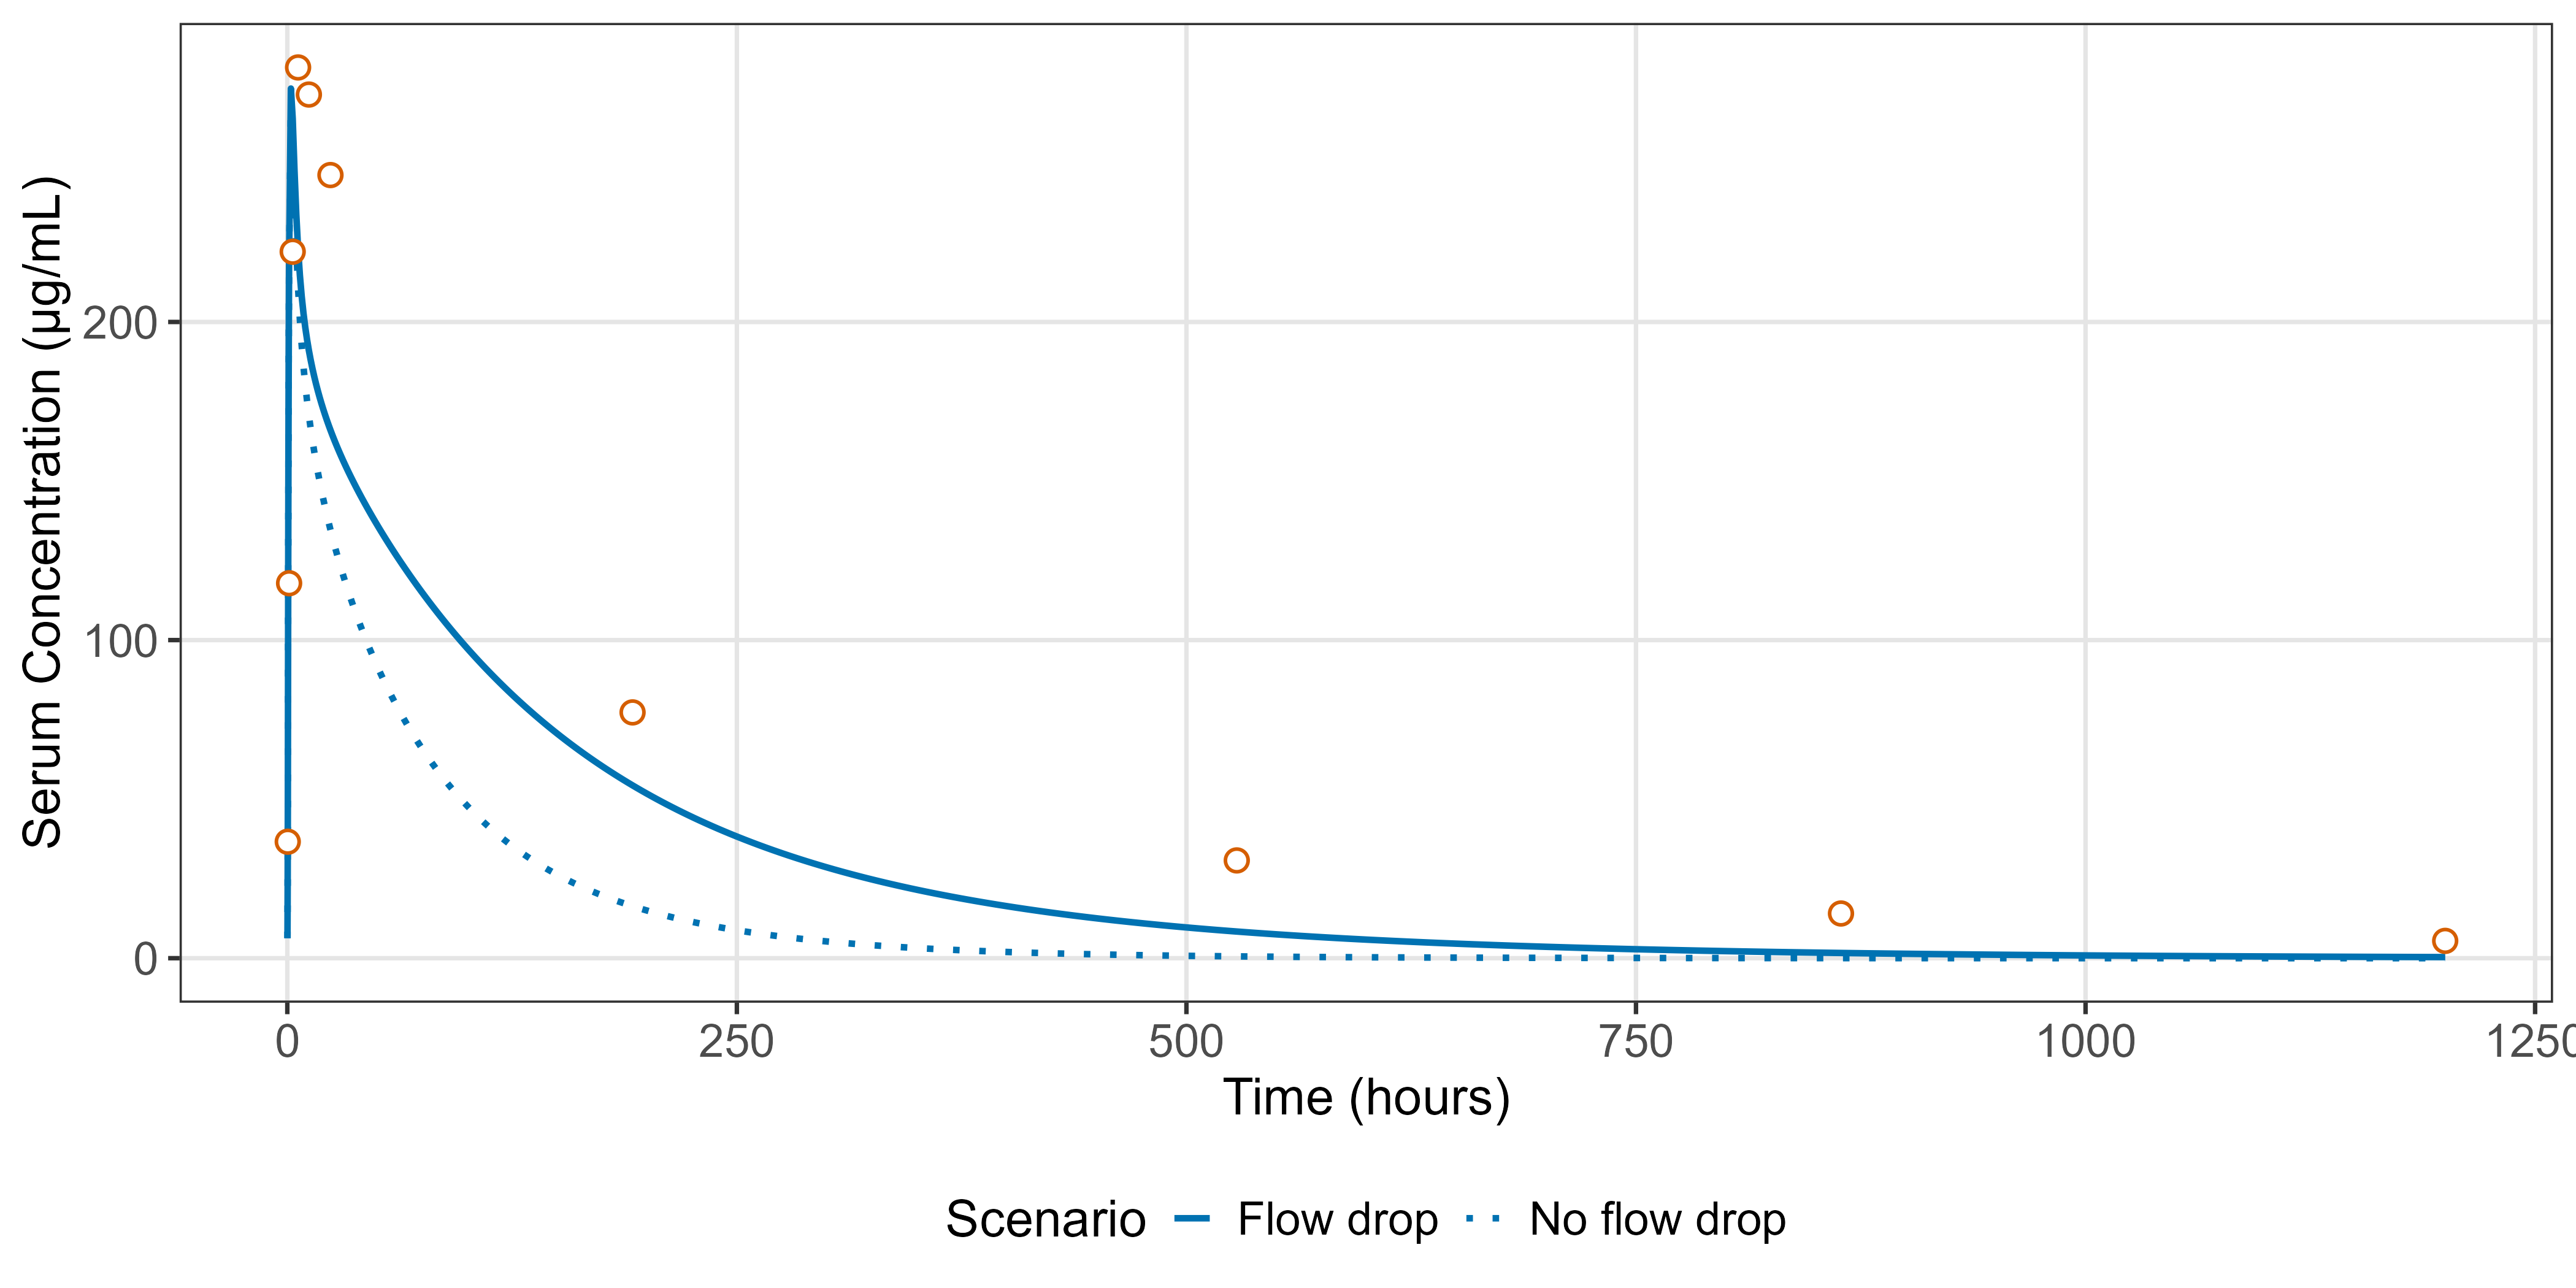
\includegraphics[width=1.0\textwidth]{sup_figures/flow_drop.png}
    \caption{Comparison of serum concentrations predicted by the model incorporating the physiological decline in renal flow (solid line) with those from a model assuming a constant flow along the renal tubule equal to the glomerular filtration rate (GFR). Simulations reproduce the experimental data of \citet{dzierlenga_2020}, where a male rat received an oral dose of 48 mg/kg.}
    \label{fig:flow_drop}
\end{figure}

Most PBK models for PFAS in the literature assume a fixed unbound fraction and do not explicitly incorporate protein binding dynamics. In this study, the latter approach was adopted because some experiments involved extremely high doses. For instance, \citet{dzierlenga_2020} administered doses to female rats as high as 320 mg/kg. Figure \ref{fig:fu_plot} illustrates how the plasma unbound fraction varies over time across the doses tested in the calibration studies. Except for the highest dose of 320 mg/kg, a fixed unbound fraction would have been adequate.


\begin{figure}[H]
    \centering
    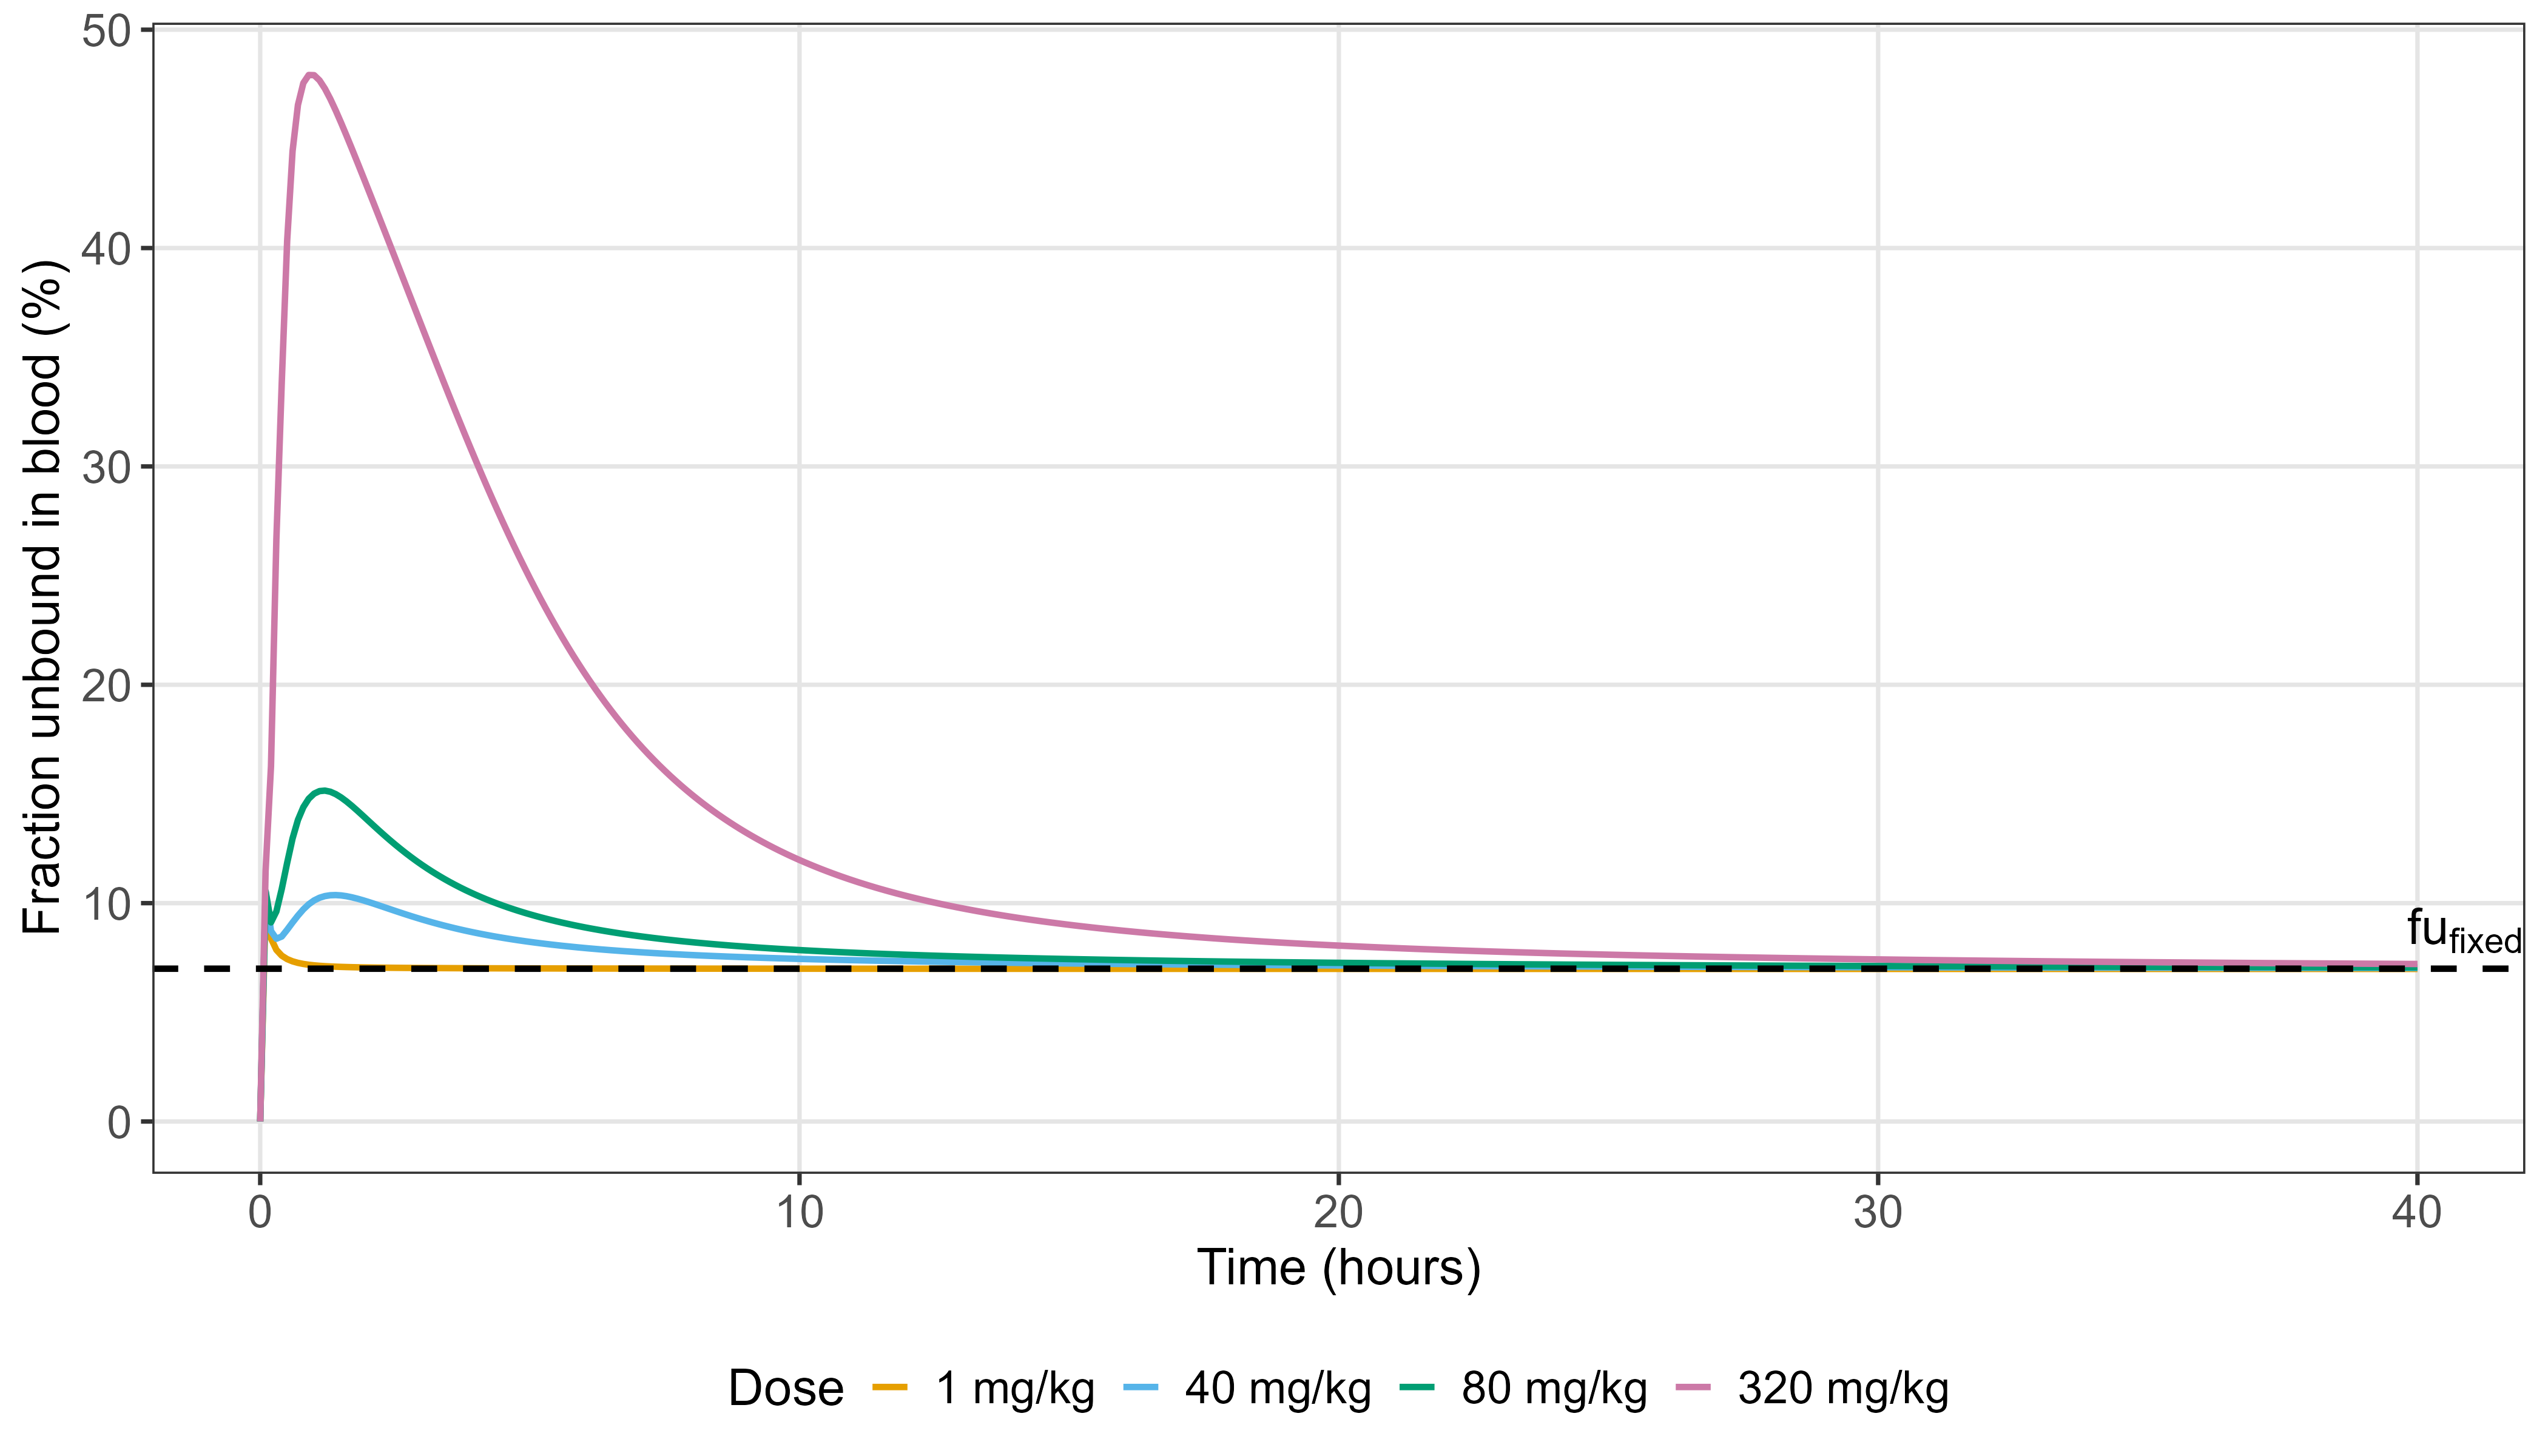
\includegraphics[width=1.0\textwidth]{sup_figures/fu_plot.png}
    \caption{Evolution of the unbound plasma fraction of PFOA in female rats across doses reported in the calibration studies.}
    \label{fig:fu_plot}
\end{figure}


A broad spectrum of PFOA association constant values to albumin is reported in the literature, ranging from $6 \cdot 10^2$ \citep{macmanuspencer_2010} to $9 \cdot 10^6$ \citep{crisalli_2023}, due to differences in measurement methods and experimental conditions. This is the major reason why the association constant was estimated from data and not taken from the literature. The fraction unbound in rat plasma reported in \citep{ryu_2024b}, which is similar to the one reported in \citep{smeltz_2023}, was used as a safe way to derive an albumin association constant and compare the resulting serum profiles between a model that employs the estimated albumin association constant and one that uses this literature-derived value. Assuming that the concentration of PFOA is significantly smaller than the concentration of available albumin, the association constant, $Ka$, can be calculated as follows:

\begin{align}
\begin{aligned}
Ka = \frac{1-f_u}{f_u \cdot C_{alb}}
\end{aligned} 
\end{align}

\noindent
where $C_{alb}$ is the albumin concentration, assumed equal to 555 $ \text{umol}/\text{L}$ \citep{rose_2015} and $f_u$ set equal to 0.003 \citep{ryu_2024b}. Based on the formula above, the association constant that reproduces the experimentally derived unbound fraction is approximately $5.5 \cdot 10^5$ L/mol. Figure \ref{fig:protein_binding} compares the predicted plasma concentrations obtained with this literature-derived value to those obtained with the calibrated value of $2.4 \cdot 10^4$ L/mol. Using the literature value results in substantially lower clearance than observed in the data, whereas the calibrated lower association constant provides a much closer match.

\begin{figure}[H]
    \centering
    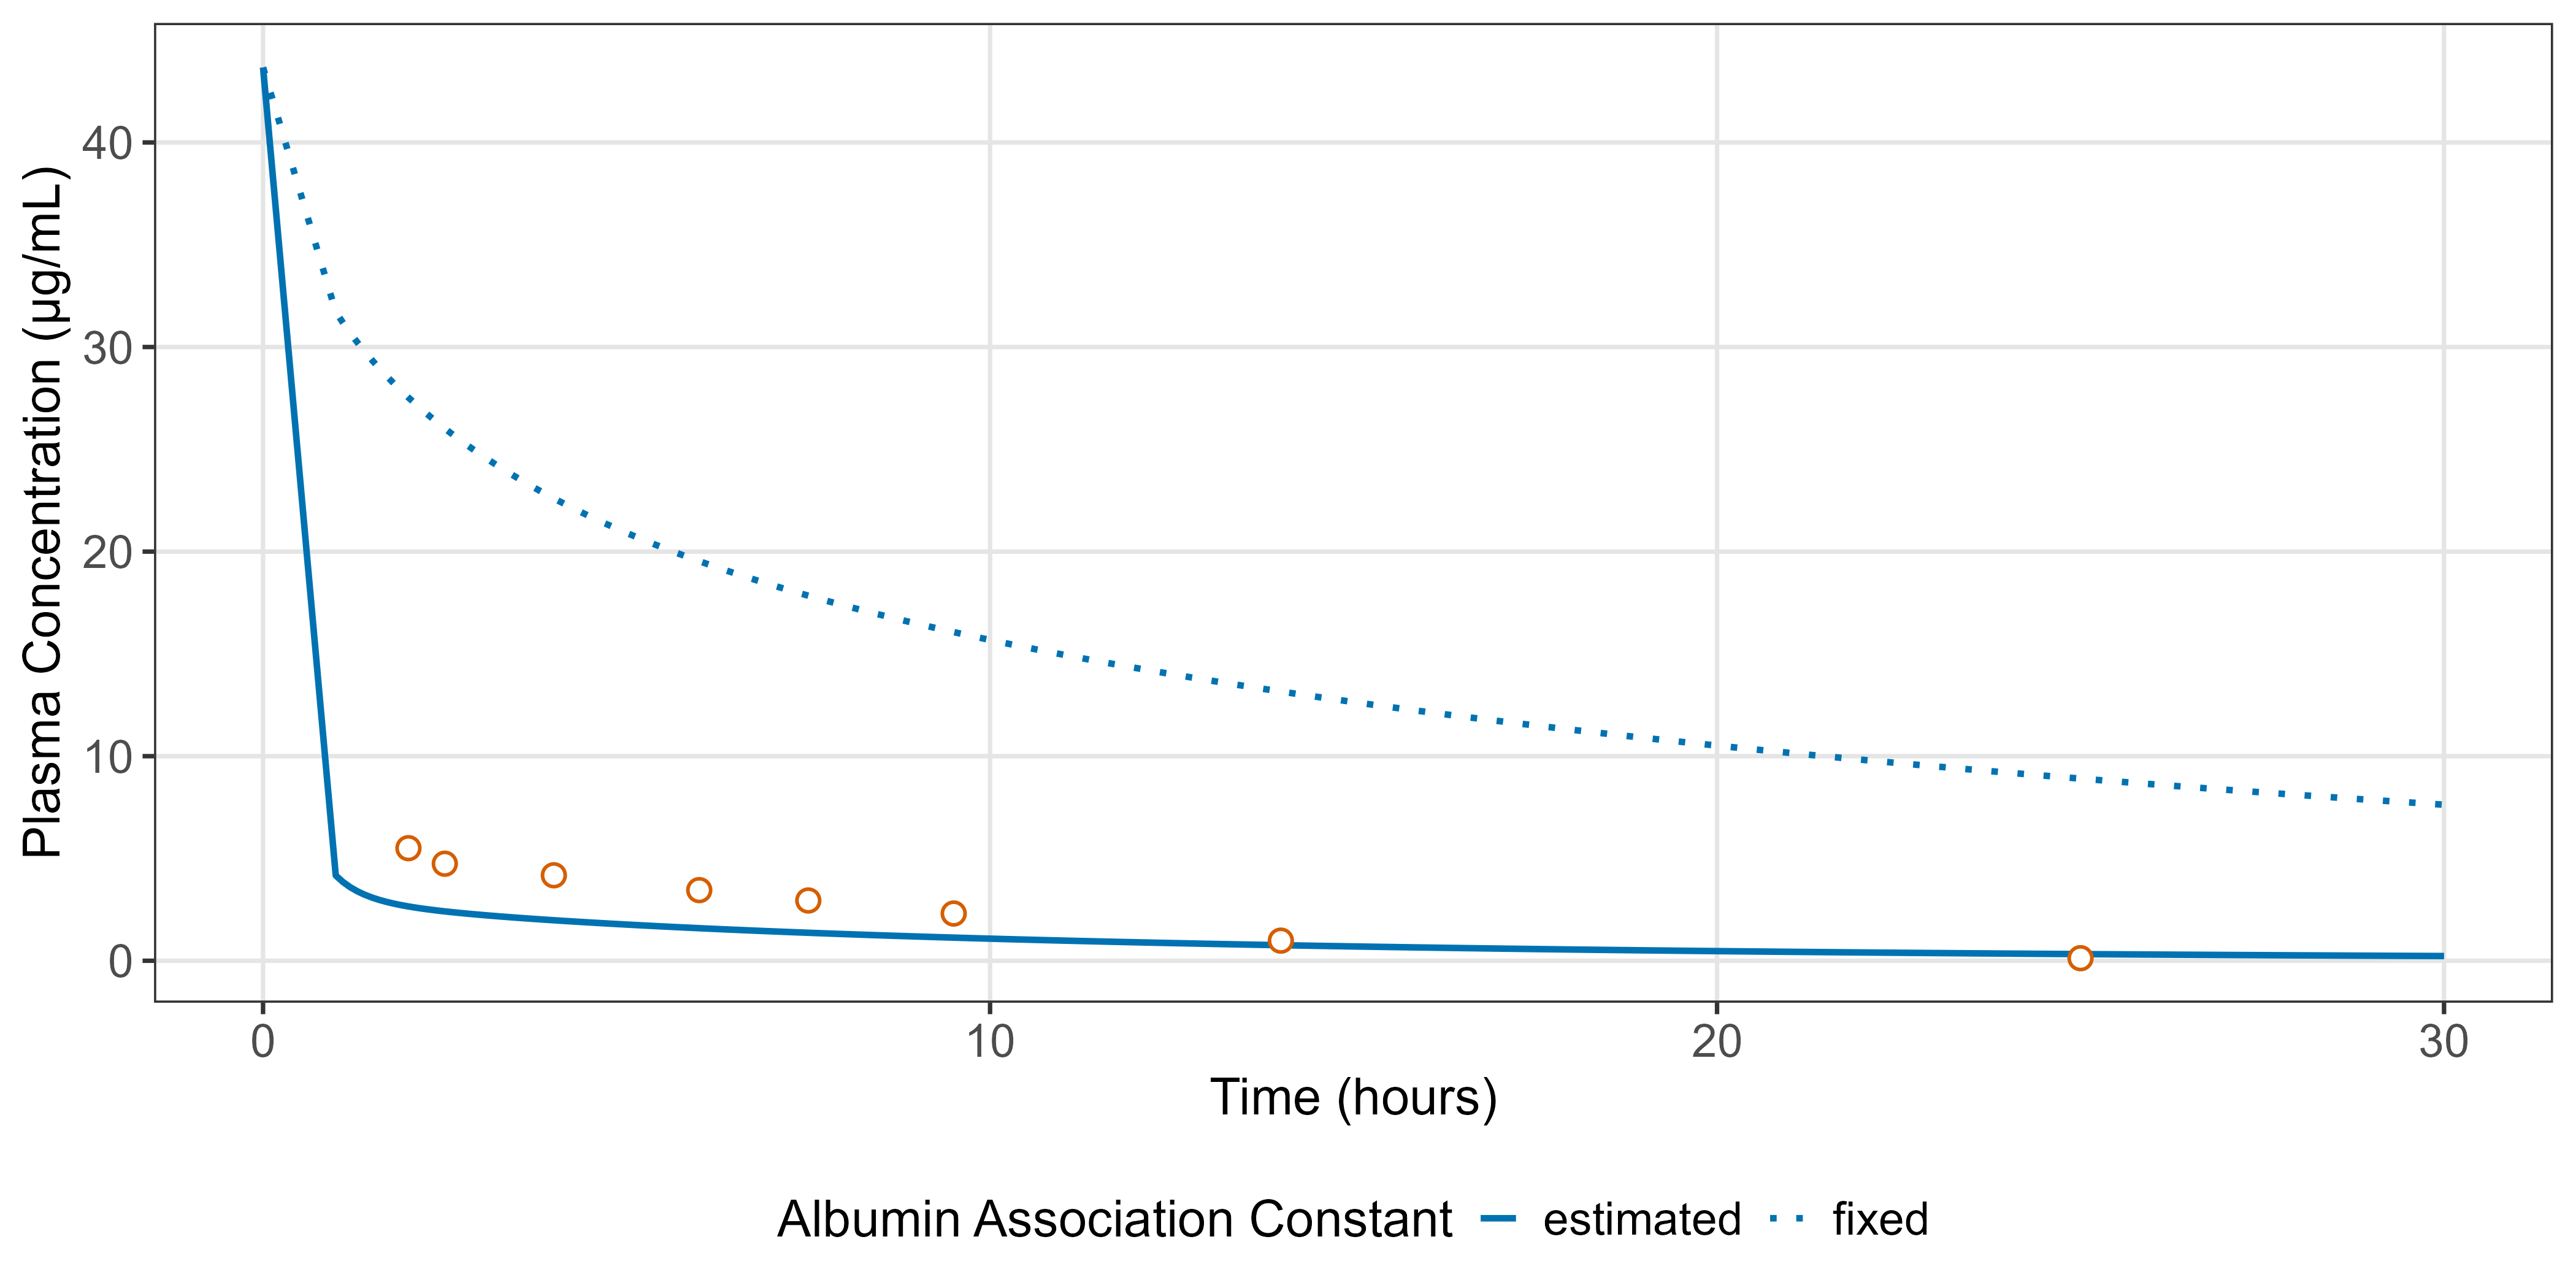
\includegraphics[width=1.0\textwidth]{sup_figures/protein_binding.png}
    \caption{Comparison of plasma concentrations predicted by the model using the predicted albumin association constant (solid line), equal to $3 \cdot 10^4$ $\text{L}/\text{mol}$ with those from a model that uses an albumin association constant equal to $5.8 \cdot 10^5$ $\text{L}/\text{mol}$, estimated using the \textit{in vitro} fraction unbound data from \citet{ryu_2024b}. Simulations reproduce the experimental data of \citet{kim_2016}, where a female rat received an IV dose of 1 mg/kg.}
    \label{fig:protein_binding}
\end{figure}


Finally, Figure \ref{fig:paracellular} highlights the role of paracellular diffusion in shaping model dynamics. When only transcellular transport is considered, using the apparent permeability value from the monolayer experiment of \citet{ryu_2024}, the predicted amount reaching the liver tissue is negligible compared with the corresponding \textit{in vivo} measurements. This suggests that either the \textit{in vitro}-derived permeability is not suitable for parameterising transcellular transport across the endothelium, or that paracellular transport constitutes the dominant pathway for PFOA diffusion across the endothelium.

\begin{figure}[H]
    \centering
    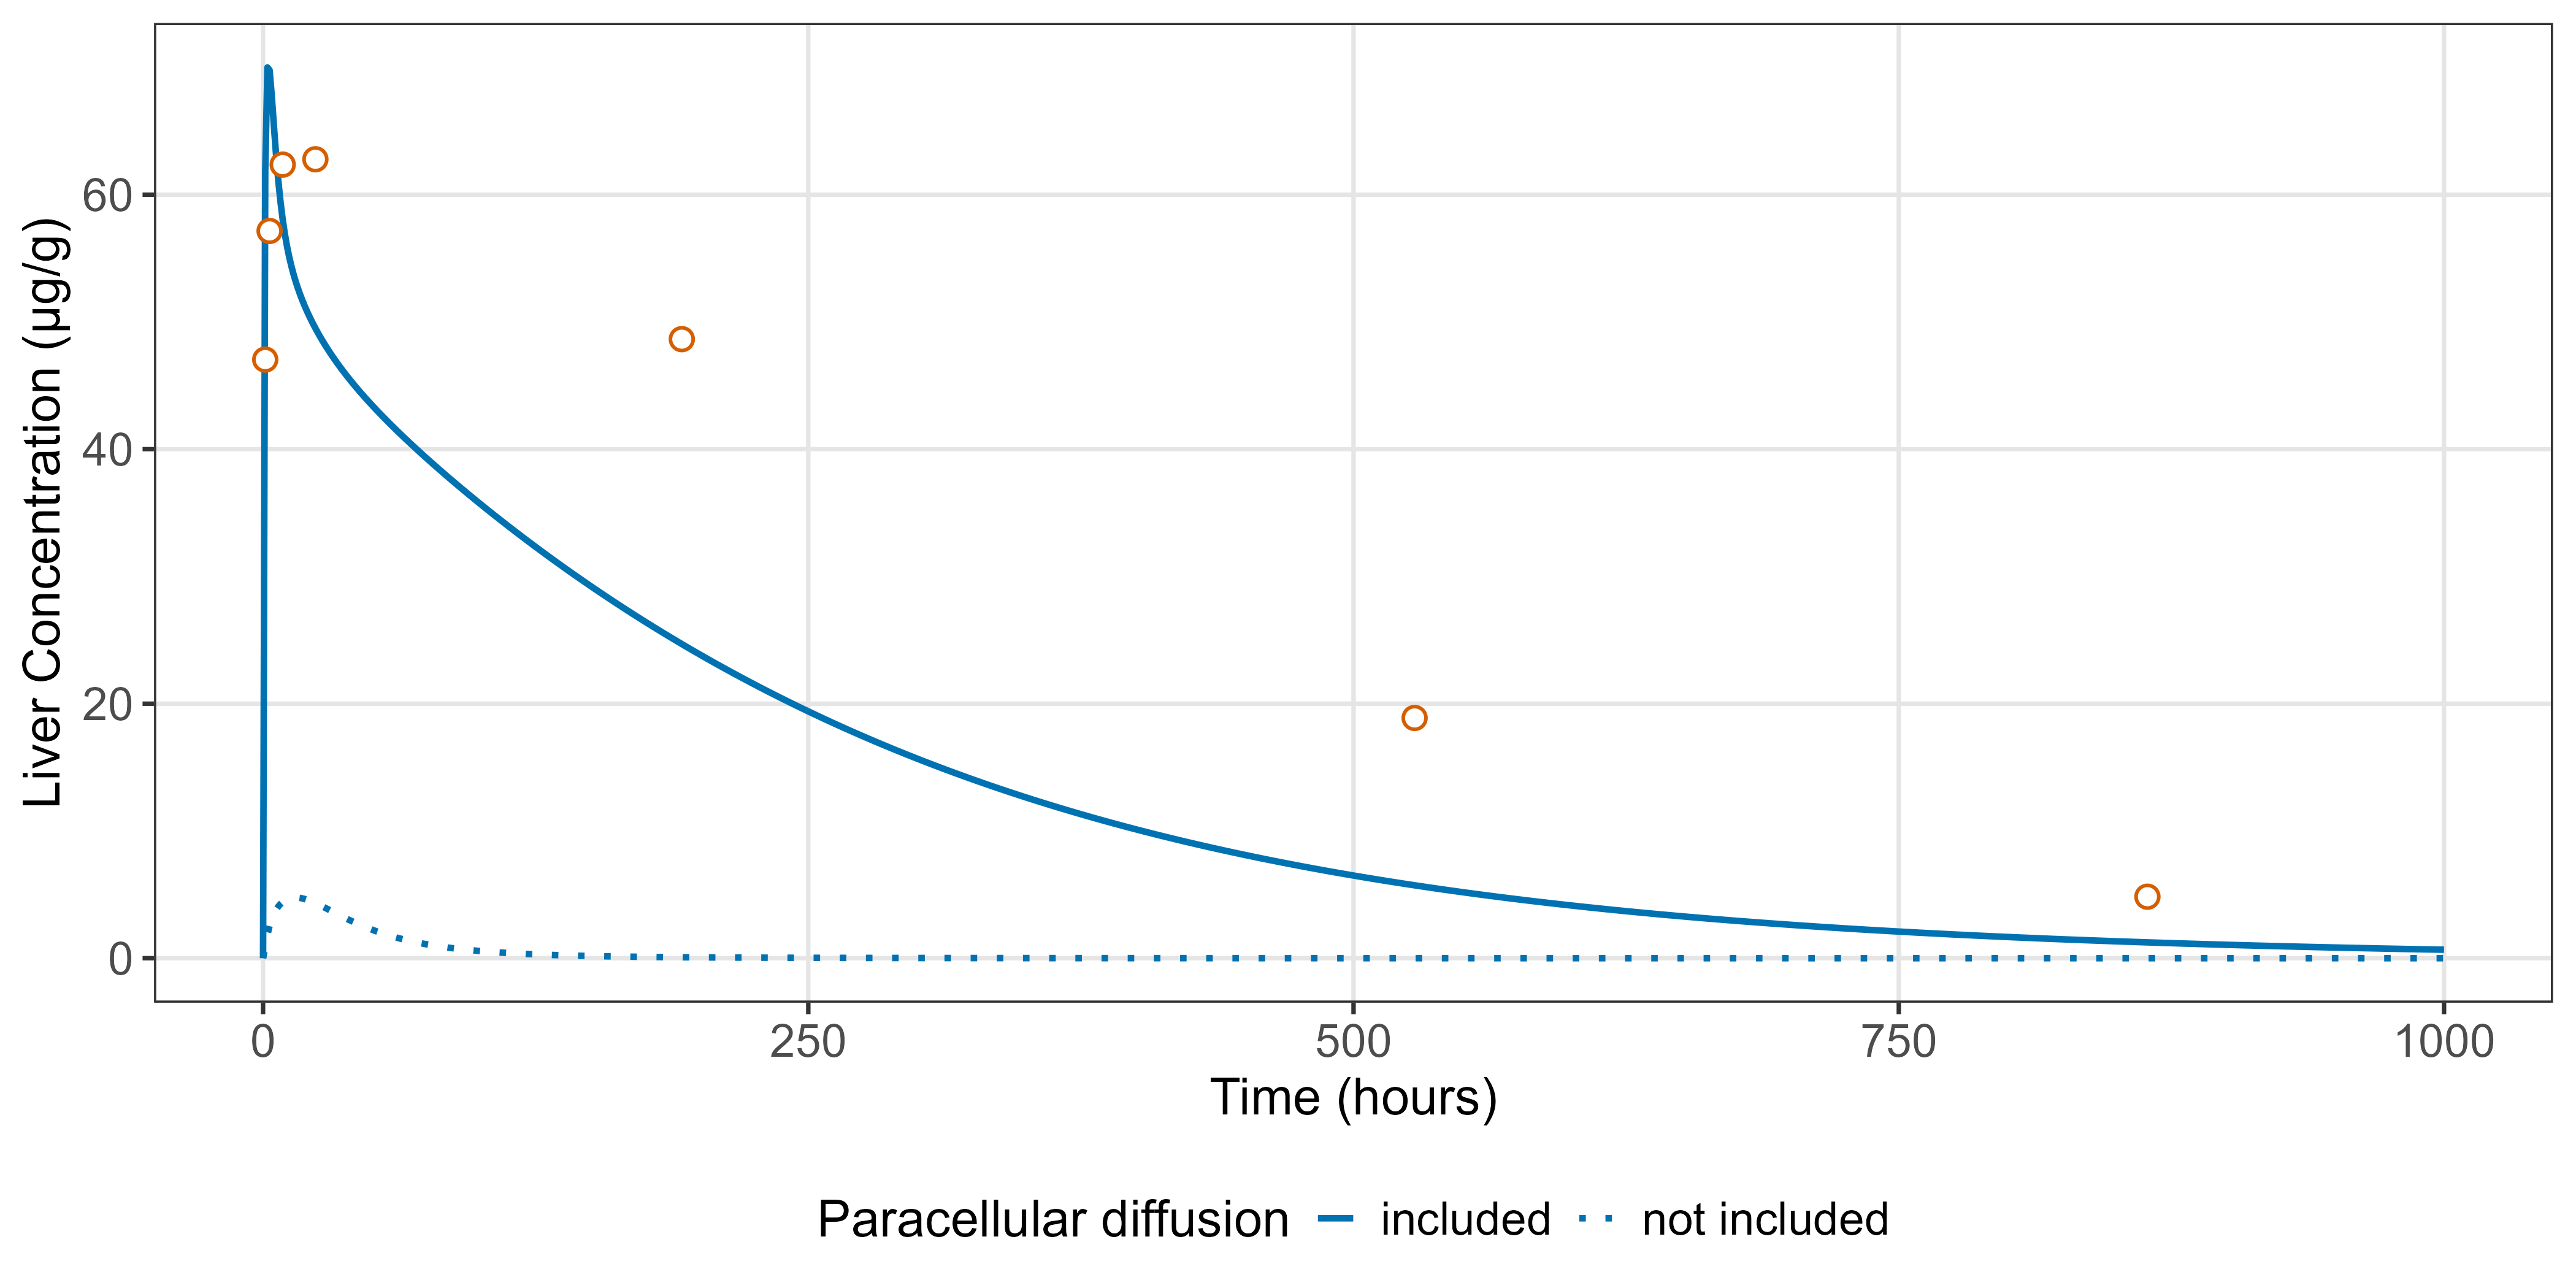
\includegraphics[width=1.0\textwidth]{sup_figures/paracellular_diffusion.png}
    \caption{Comparison of liver concentrations predicted by the model using transcellular and paracellular diffusion (solid line), with those from a model that uses only transcellular diffusion, using the in vitro permeability data from \citet{ryu_2024}. Simulations reproduce the experimental data of \citet{dzierlenga_2020}, where a male rat received an oral dose of 12 mg/kg.}
    \label{fig:paracellular}
\end{figure}

\newpage
\bibliographystyle{apalike}  
\bibliography{Bibliography}

\end{document}


